
% Encoding: UTF-8
%%%%%%%%%%%%%%%%%%%%%%%%%%%%%%%%%%%%%%%%%%%%%%%%%%%%%%%%%%%%%%%%%%%%%%%%%%%%%%%

%%%%%%%%%%%%%%%%%%%%%%%%%%%%%%%%%%%%%%%%%%%%%%%%%%%%%%%%%%%%%%%%%%%%%%%%%%%%%%%
% $Id: slides.tex 17 2011-02-10 15:21:56Z klugeflo $
%%%%%%%%%%%%%%%%%%%%%%%%%%%%%%%%%%%%%%%%%%%%%%%%%%%%%%%%%%%%%%%%%%%%%%%%%%%%%%%

%%%%%%%%%%%%%%%%%%%%%%%%%%%%%%%%%%%%%%%%%%%%%%%%%%%%%%%%%%%%%%%%%%%%%%%%%%%%%%%
%%
%% Vorlage fuer LaTeX-Beamer
%% gemaess dem Corporate Design der Uni Augsburg
%%
%%%%%%%%%%%%%%%%%%%%%%%%%%%%%%%%%%%%%%%%%%%%%%%%%%%%%%%%%%%%%%%%%%%%%%%%%%%%%%%
%%
%% Changelog:
%%
%% 11/02/10 (FAK) Start
%%
%%%%%%%%%%%%%%%%%%%%%%%%%%%%%%%%%%%%%%%%%%%%%%%%%%%%%%%%%%%%%%%%%%%%%%%%%%%%%%%


%%%%%%%%%%%%%%%%%%%%%%%%%%%%%%%%%%%%%%%%%%%%%%%%%%%%%%%%%%%%%%%%%%%%%%%%%%%%%%%

\documentclass[xcolor=pdftex,dvipsnames,table]{beamer}
\setbeamertemplate{navigation symbols}{}%remove navigation symbols
%%%%%%%%%%%%%%%%%%%%%%%%%%%%%%%%%%%%%%%%%%%%%%%%%%%%%%%%%%%%%%%%%%%%%%%%%%%%%%%

% Language settings
% IMPORTANT: If you change the language settings, make sure to run
% cleantex prior to any latex/pdflatex to remove all .aux files, else
% latex might fail!
\usepackage[english]{babel}
%\usepackage[german]{babel}

\usepackage{pdfpages}
\usepackage{graphicx}
\usepackage{tikz}
\usepackage[utf8]{inputenc}
%\usepackage{mathptmx}


%%%%%%%%%%%%%%%%%%%%%%%%%%%%%%%%%%%%%%%%%%%%%%%%%%%%%%%%%%%%%%%%%%%%%%%%%%%%%%%

%\usetheme{fai}

% IMPORTANT/TODO: currently only PDF graphic files should be used, PNG
% or JPEG may harm the Adobe Reader colour palette and result in
% strange display colours.
%\DeclareGraphicsExtensions{.pdf}

\graphicspath{{./img/}}

%%%%%%%%%%%%%%%%%%%%%%%%%%%%%%%%%%%%%%%%%%%%%%%%%%%%%%%%%%%%%%%%%%%%%%%%%%%%%%%
%% Presentation main settings
%%%%%%%%%%%%%%%%%%%%%%%%%%%%%%%%%%%%%%%%%%%%%%%%%%%%%%%%%%%%%%%%%%%%%%%%%%%%%%%

\title{Systemnahe Informatik}
\subtitle{Übungsgruppe Xeon Phi}
\author{Dominik Walter}
\date{Sommersemester 2018}


%%%%%%%%%%%%%%%%%%%%%%%%%%%%%%%%%%%%%%%%%%%%%%%%%%%%%%%%%%%%%%%%%%%%%%%%%%%%%%%
%% Main Document starts here
%%%%%%%%%%%%%%%%%%%%%%%%%%%%%%%%%%%%%%%%%%%%%%%%%%%%%%%%%%%%%%%%%%%%%%%%%%%%%%%



\begin{document}

\begin{frame}
	\frametitle{\ }
	\titlepage
\end{frame}
%{
%\section{Titlepage}
%
%	\usebackgroundtemplate%
%	{%
%%	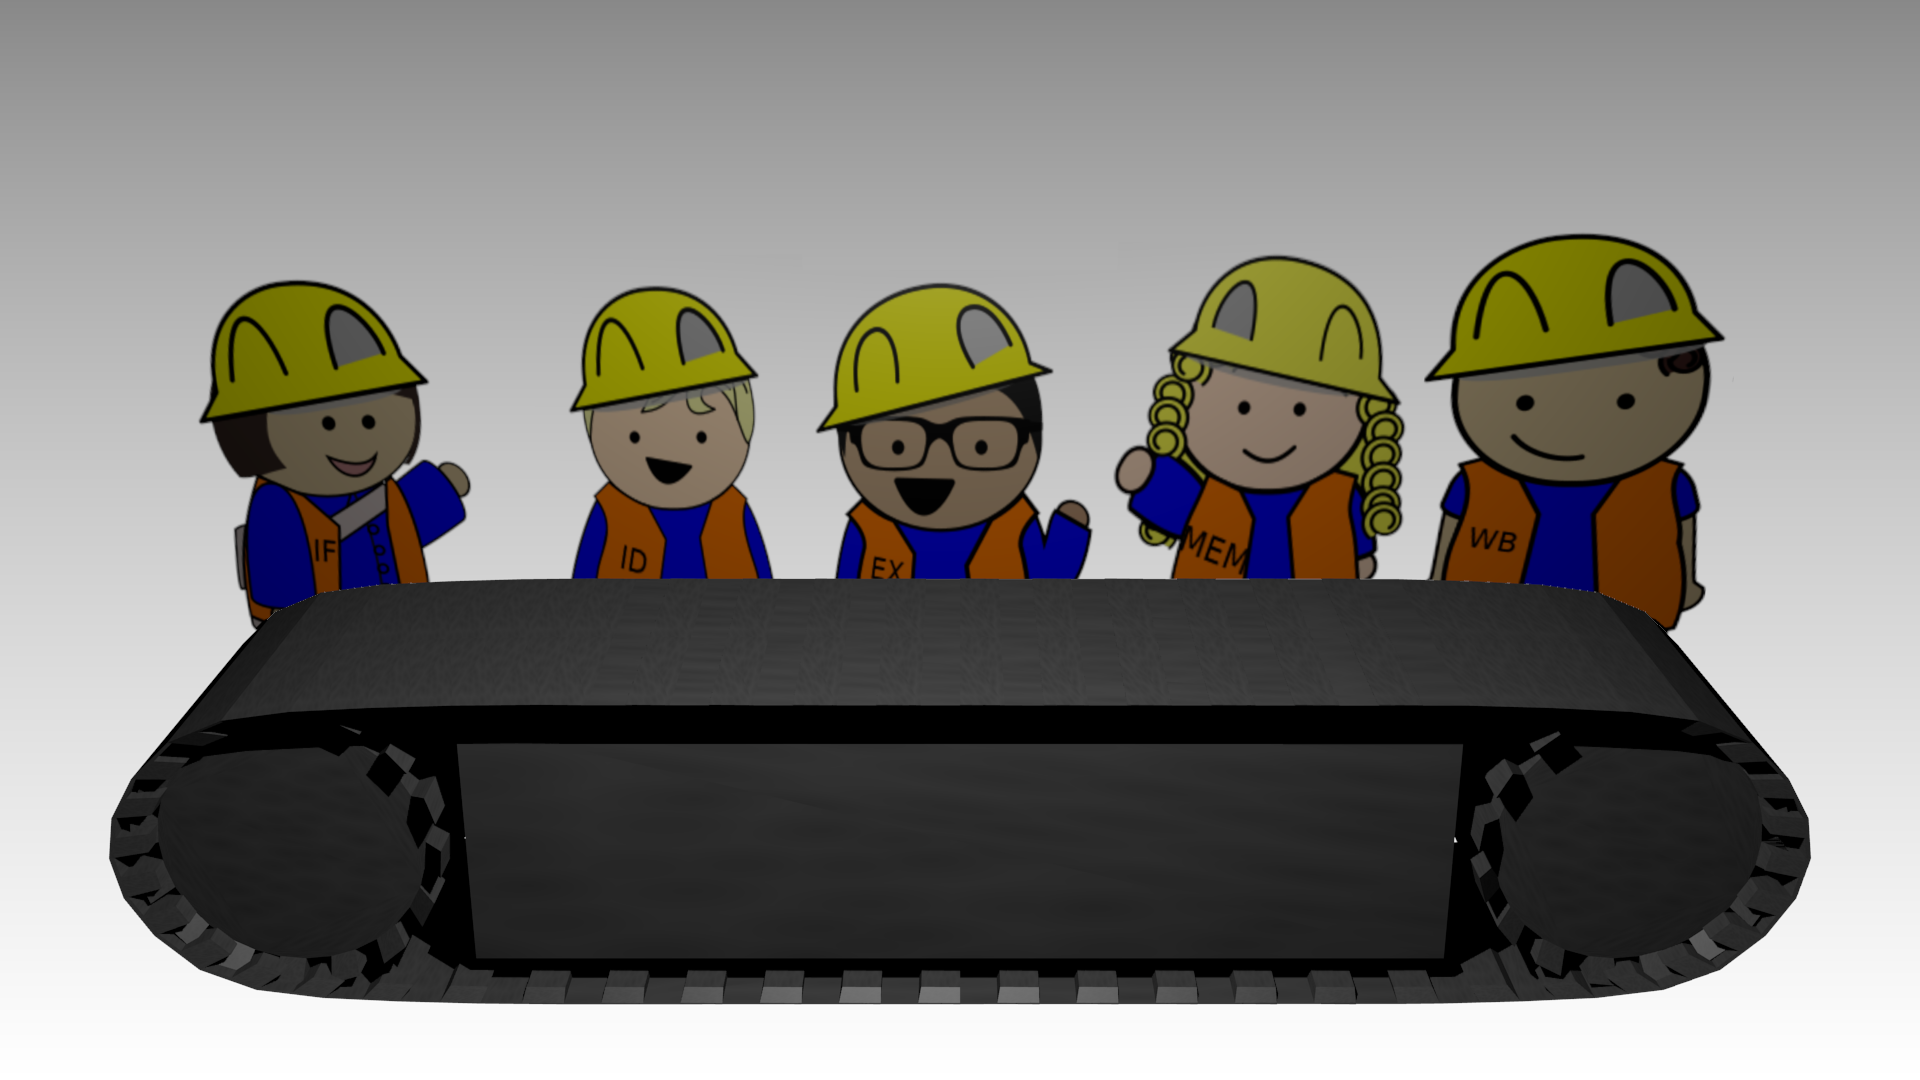
\includegraphics[width=\paperwidth,height=\paperheight]{final}%
%	}
%\begin{frame}
%%\phantom{empty}
%%\phantom{empty}
%%\phantom{empty}
%%\phantom{empty}
%%\phantom{empty}
%%\phantom{empty}
%%\phantom{empty}
%%\color{white}
%		\huge
%		\centering
%		\underline{RISCV-Pipeline}
%		\large
%		\\Systemnahe Informatik
%		\small
%		\\Übungsgruppe Xeon Phi
%		%Dominik Walter
%		
%		%08.02.2018
%
%
%\end{frame}
%
%}
%%%%%%%%%%%%%%%%%%%%%%%%%%%%%%%%%%%%%%%%%%%%%%%%%%%%%%%%%%%%%%%%%%%%%%%%%%%%%%%

%%%%%%%%%%%%%%%%%%%%%%%%%%%%%%%%%%%%%%%%%%%%%%%%%%%%%%%%%%%%%%%%%%%%%%%%%%%%%%%

\section{Allgemein}

\begin{frame}
	\frametitle{Intel Skylake}
	\begin{figure}
		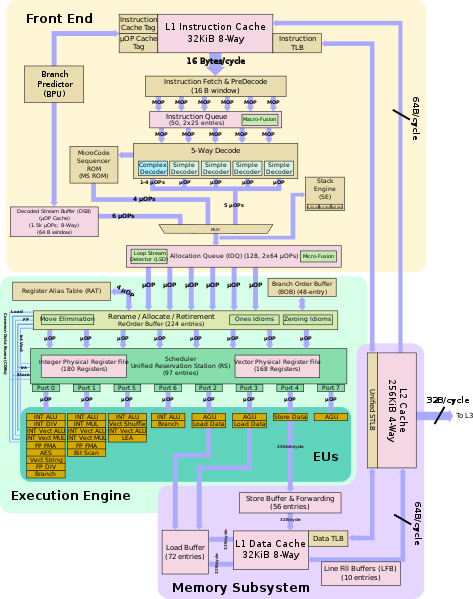
\includegraphics[width=0.5\textwidth]{skylake.png}
		\caption{
			https://en.wikichip.org/wiki/File:skylake\_block\_diagram.svg}
	\end{figure}
\end{frame}



\begin{frame}
	\frametitle{RISCV Pipeline}
	\begin{picture}(0,0)
	\put(-30,-40){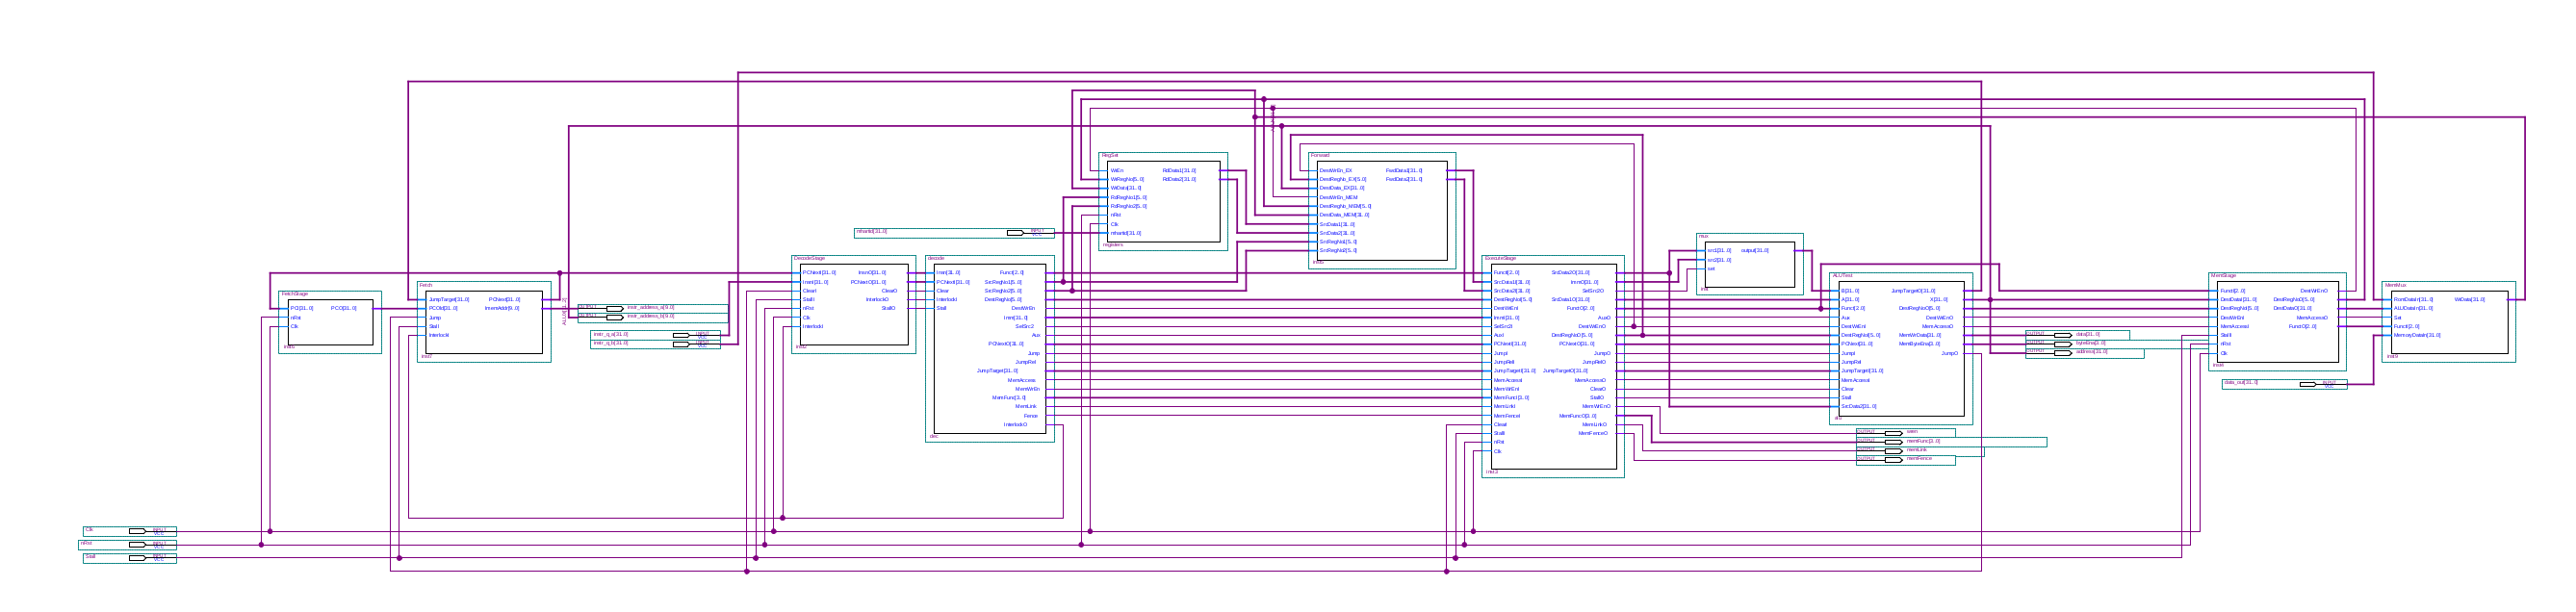
\includegraphics[width=1.2\textwidth]{core.png}}
	\end{picture}
\end{frame}

%%=============================================================================
\begin{frame}
	\frametitle{RISCV Pipeline}
	\begin{picture}(0,0)
	\put(0,-85){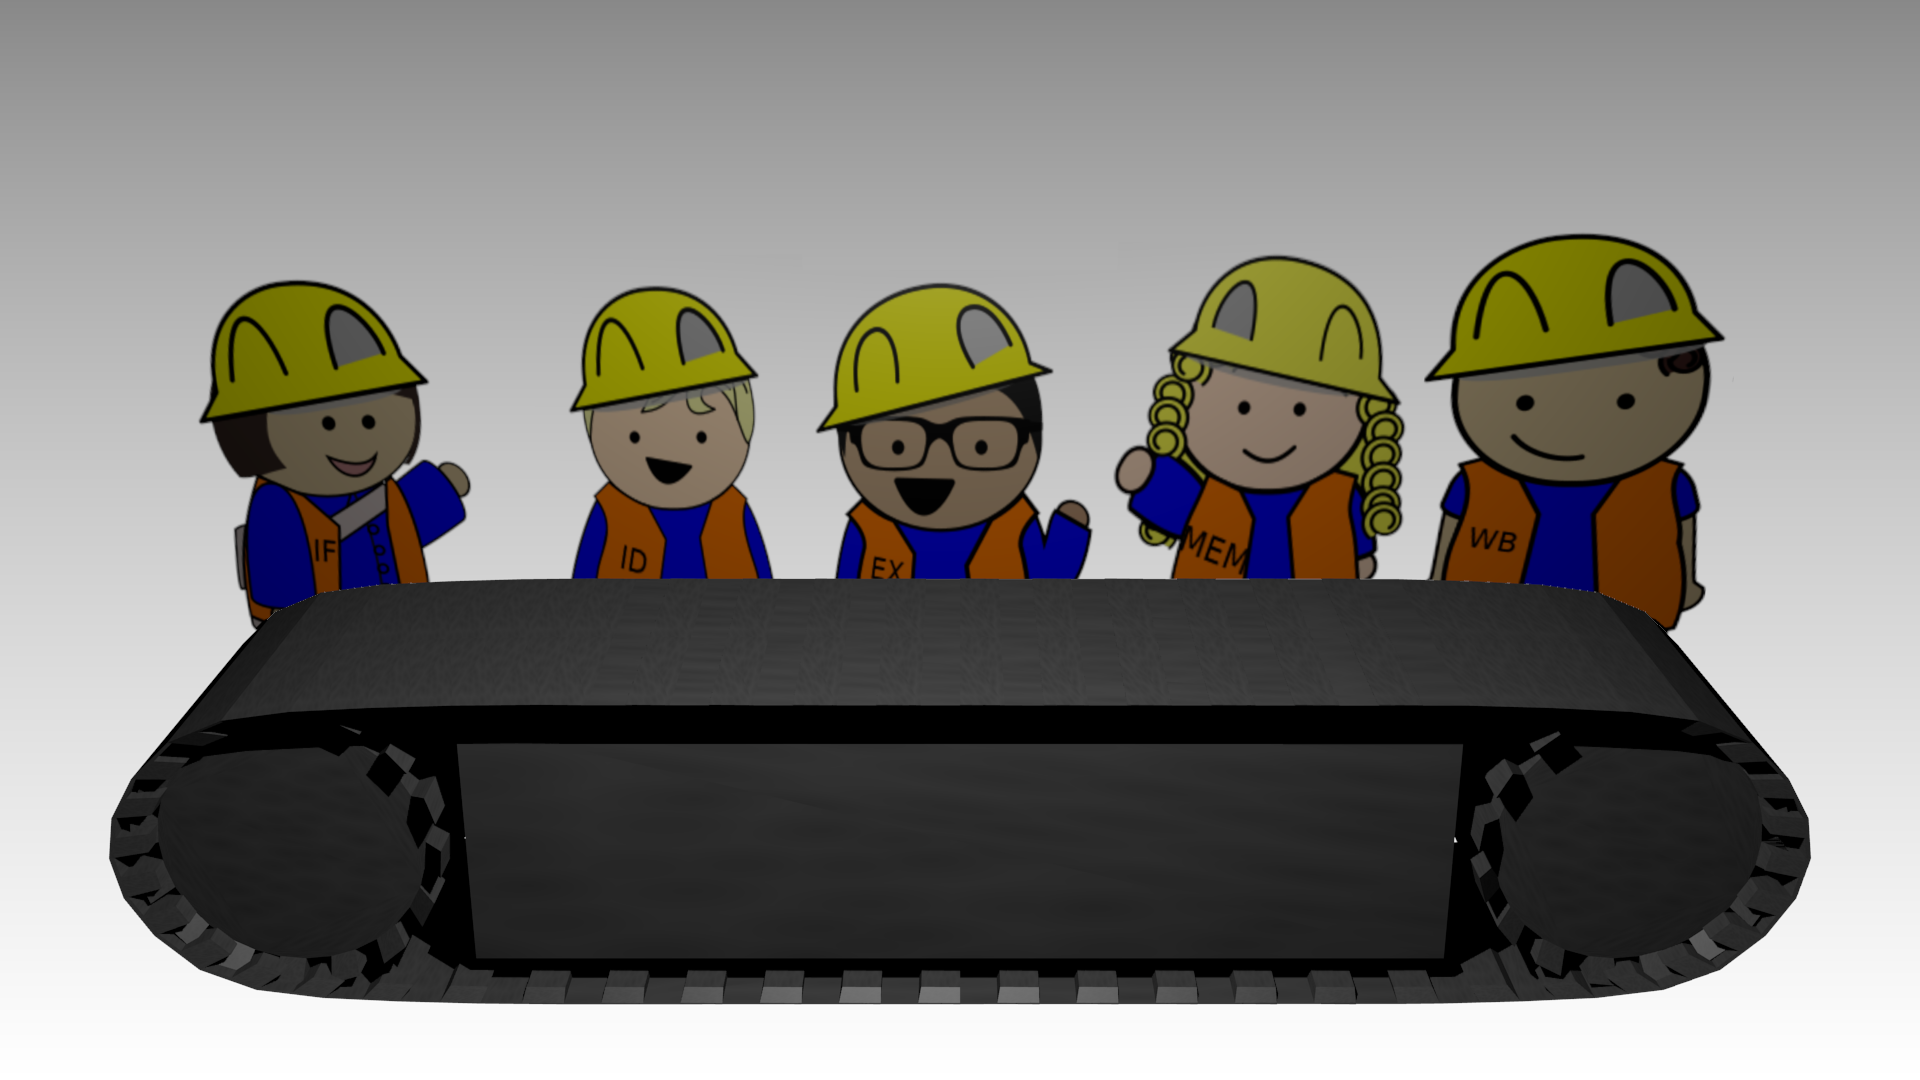
\includegraphics[width=1.0\textwidth]{final.png}}
	%FETCH
	\put(50,-12){\tiny\color{white}}
	
	%DECODE
	\put(90,-12){\tiny\color{white}}
	\put(90,-17){\tiny\color{white}}
	
	%EXECUTE
	\put(135,-12){\tiny\color{white}}
	\put(135,-17){\tiny\color{white}}
	\put(135,-22){\tiny\color{white}}
	
	%MEMORY
	\put(185,-12){\tiny\color{white}}
	\put(185,-17){\tiny\color{white}}
	\put(185,-22){\tiny\color{white}}
	
	%WRITEBACK
	\put(225,-12){\tiny\color{white}}
	\put(225,-17){\tiny\color{white}}
	\put(225,-22){\tiny\color{white}}
	
	%REGISTERS
	\put(80,-37){\tiny\color{white}zero = 0}
	\put(80,-42){\tiny\color{white}ra = 0}
	\put(80,-47){\tiny\color{white}sp = 0}
	\put(80,-52){\tiny\color{white}pc = 0}
	\put(80,-57){\tiny\color{white}t0 = 0}
	\put(80,-62){\tiny\color{white}t1 = 0}
	
	\put(110,-37){\tiny\color{white}t2 = 0}
	\put(110,-42){\tiny\color{white}t3 = 0}
	\put(110,-47){\tiny\color{white}t4 = 0}
	\put(110,-52){\tiny\color{white}t5 = 0}
	\put(110,-57){\tiny\color{white}t6 = 0}
	\put(110,-62){\tiny\color{white}a0 = 0}
	
	\put(140,-37){\tiny\color{white}a1 = 0}
	\put(140,-42){\tiny\color{white}a2 = 0}
	\put(140,-47){\tiny\color{white}a3 = 0}
	\put(140,-52){\tiny\color{white}a4 = 0}
	\put(140,-57){\tiny\color{white}a5 = 0}
	\put(140,-62){\tiny\color{white}a6 = 0}
	
	\put(170,-37){\tiny\color{white}a7 = 0}
	\put(170,-42){\tiny\color{white}s1 = 0}
	\put(170,-47){\tiny\color{white}s2 = 0}
	\put(170,-52){\tiny\color{white}s3 = 0}
	\put(170,-57){\tiny\color{white}s4 = 0}
	\put(170,-62){\tiny\color{white}s5 = 0}
	
	\put(200,-37){\tiny\color{white}s6 = 0}
	\put(200,-42){\tiny\color{white}s7 = 0}
	\put(200,-47){\tiny\color{white}s8 = 0}
	\put(200,-52){\tiny\color{white}s9 = 0}
	\put(200,-57){\tiny\color{white}s10 = 0}
	\put(200,-62){\tiny\color{white}s11 = 0}
	
	\end{picture}
\end{frame}

\begin{frame}
	\frametitle{Instruction Fetch}
	\begin{picture}(0,0)
	\put(0,-85){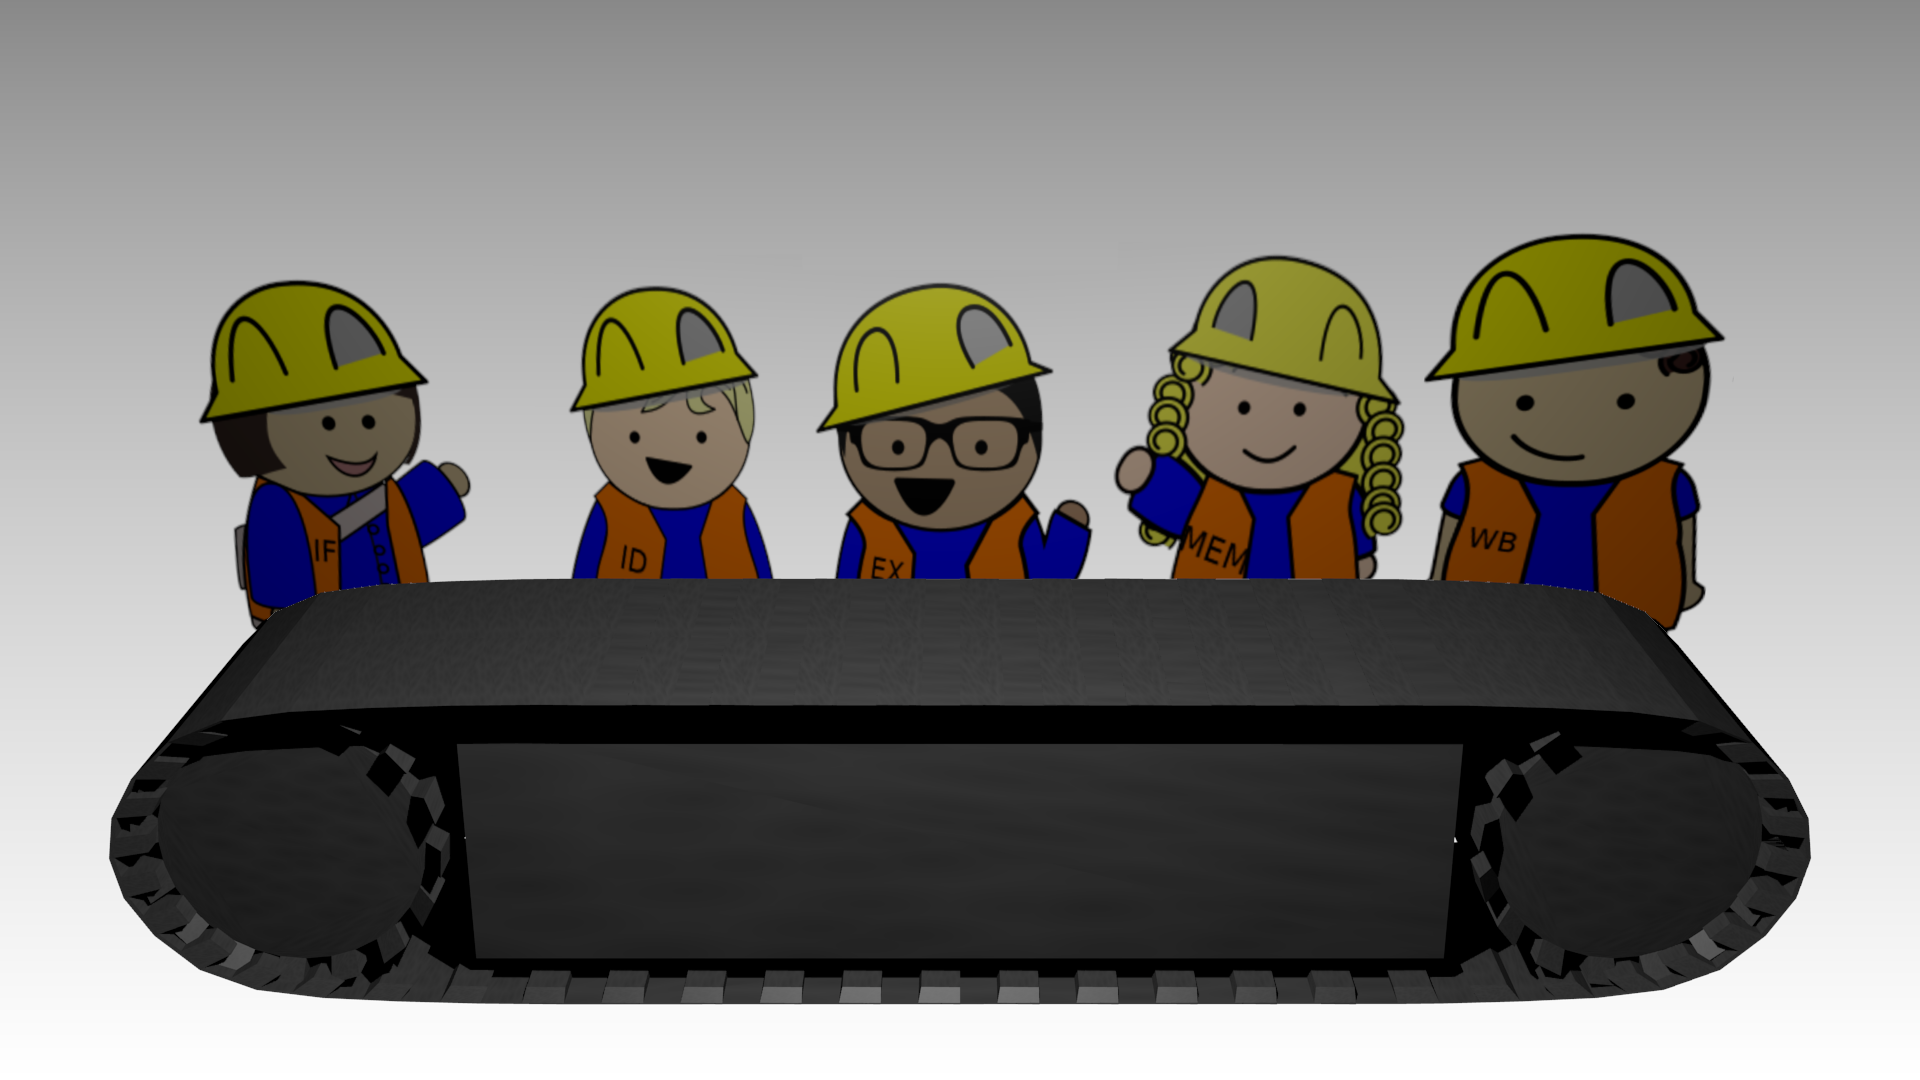
\includegraphics[width=1.0\textwidth]{final.png}}
	%FETCH
	\put(50,-12){\tiny\color{white}add t0, t0, 1}
	
	%DECODE
	\put(90,-12){\tiny\color{white}}
	\put(90,-17){\tiny\color{white}}
	
	%EXECUTE
	\put(135,-12){\tiny\color{white}}
	\put(135,-17){\tiny\color{white}}
	\put(135,-22){\tiny\color{white}}
	
	%MEMORY
	\put(185,-12){\tiny\color{white}}
	\put(185,-17){\tiny\color{white}}
	\put(185,-22){\tiny\color{white}}
	
	%WRITEBACK
	\put(225,-12){\tiny\color{white}}
	\put(225,-17){\tiny\color{white}}
	\put(225,-22){\tiny\color{white}}
	
	%REGISTERS
	\put(80,-37){\tiny\color{white}zero = 0}
	\put(80,-42){\tiny\color{white}ra = 0}
	\put(80,-47){\tiny\color{white}sp = 0}
	\put(80,-52){\tiny\color{white}pc = 4}
	\put(80,-57){\tiny\color{white}t0 = 0}
	\put(80,-62){\tiny\color{white}t1 = 0}
	
	\put(110,-37){\tiny\color{white}t2 = 0}
	\put(110,-42){\tiny\color{white}t3 = 0}
	\put(110,-47){\tiny\color{white}t4 = 0}
	\put(110,-52){\tiny\color{white}t5 = 0}
	\put(110,-57){\tiny\color{white}t6 = 0}
	\put(110,-62){\tiny\color{white}a0 = 0}
	
	\put(140,-37){\tiny\color{white}a1 = 0}
	\put(140,-42){\tiny\color{white}a2 = 0}
	\put(140,-47){\tiny\color{white}a3 = 0}
	\put(140,-52){\tiny\color{white}a4 = 0}
	\put(140,-57){\tiny\color{white}a5 = 0}
	\put(140,-62){\tiny\color{white}a6 = 0}
	
	\put(170,-37){\tiny\color{white}a7 = 0}
	\put(170,-42){\tiny\color{white}s1 = 0}
	\put(170,-47){\tiny\color{white}s2 = 0}
	\put(170,-52){\tiny\color{white}s3 = 0}
	\put(170,-57){\tiny\color{white}s4 = 0}
	\put(170,-62){\tiny\color{white}s5 = 0}
	
	\put(200,-37){\tiny\color{white}s6 = 0}
	\put(200,-42){\tiny\color{white}s7 = 0}
	\put(200,-47){\tiny\color{white}s8 = 0}
	\put(200,-52){\tiny\color{white}s9 = 0}
	\put(200,-57){\tiny\color{white}s10 = 0}
	\put(200,-62){\tiny\color{white}s11 = 0}
	
	\end{picture}
\end{frame}

\begin{frame}
	\frametitle{Instruction Decode}
	\begin{picture}(0,0)
	\put(0,-85){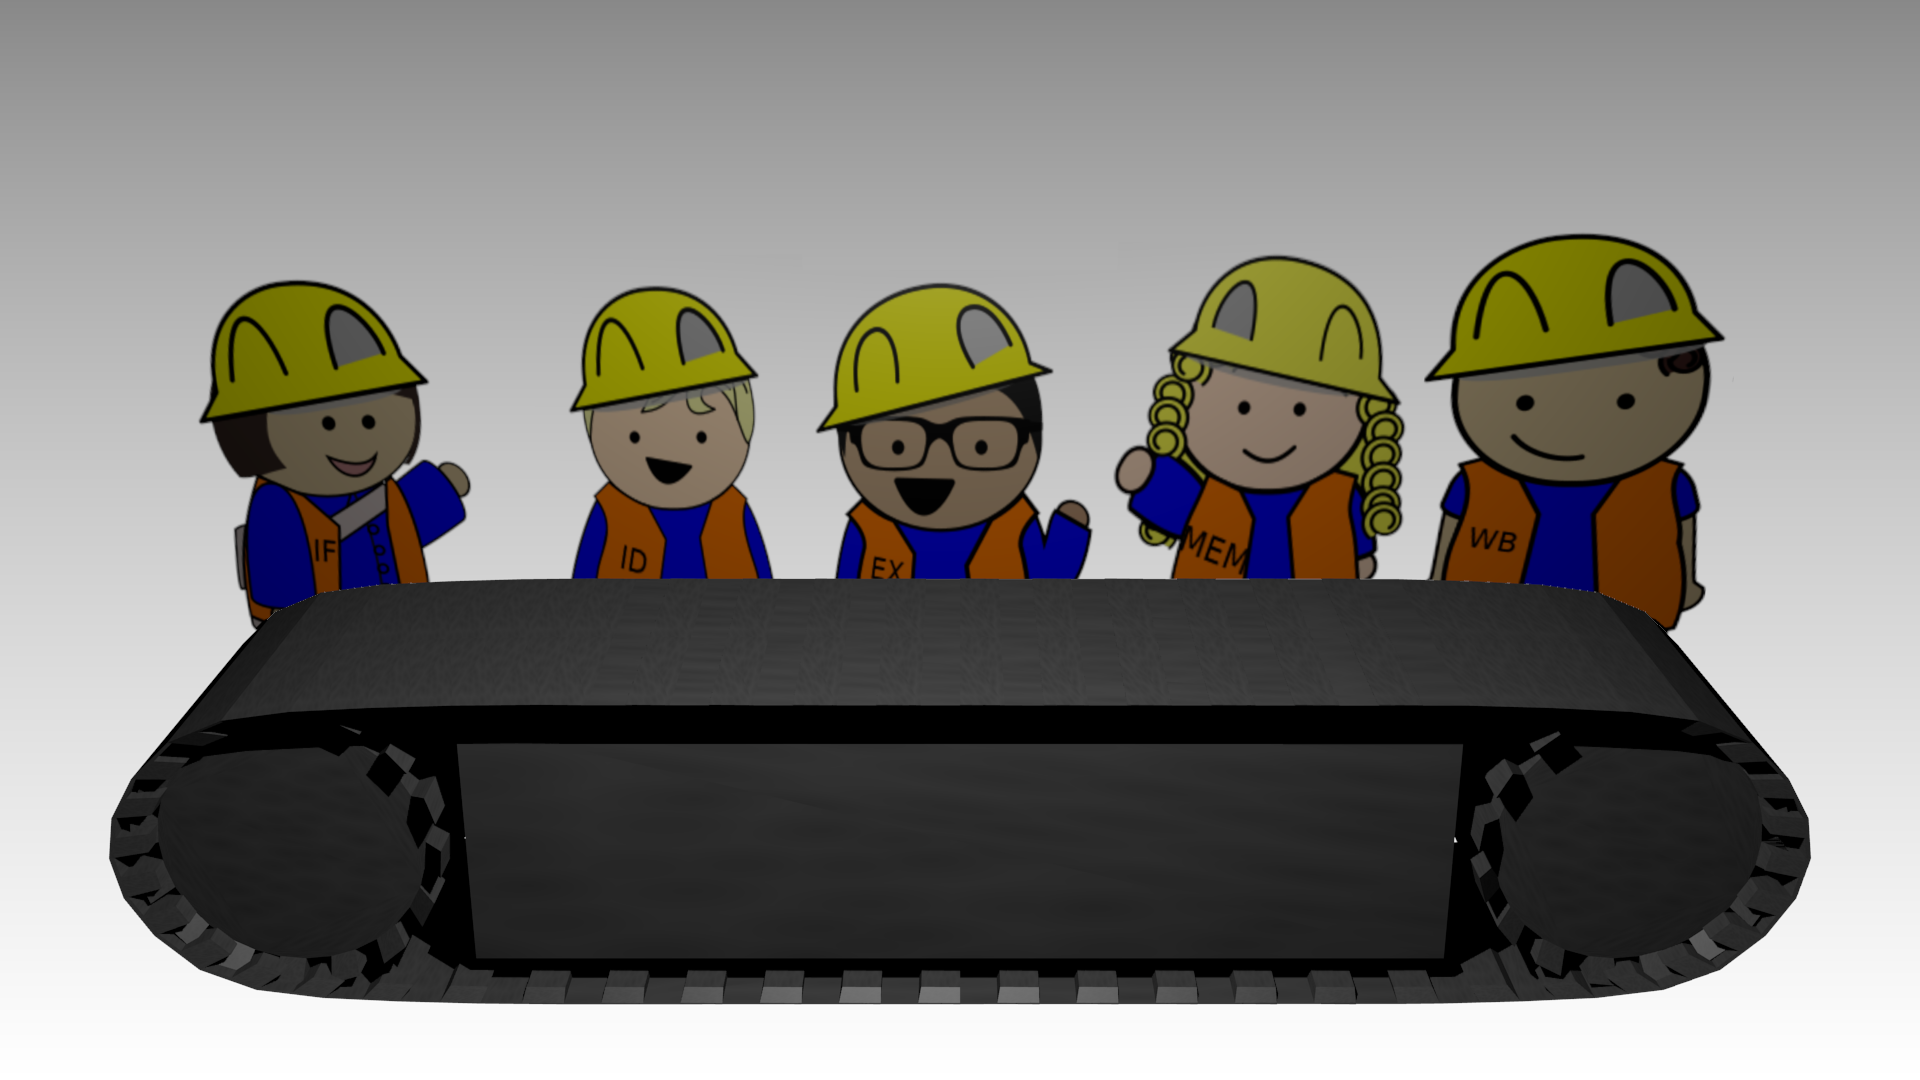
\includegraphics[width=1.0\textwidth]{final.png}}
	%FETCH
	\put(50,-12){\tiny\color{white}}
	
	%DECODE
	\put(90,-12){\tiny\color{white}add t0, t0, 1}
	\put(90,-17){\tiny\color{white}t0 = 0 + 1}
	
	%EXECUTE
	\put(135,-12){\tiny\color{white}}
	\put(135,-17){\tiny\color{white}}
	\put(135,-22){\tiny\color{white}}
	
	%MEMORY
	\put(185,-12){\tiny\color{white}}
	\put(185,-17){\tiny\color{white}}
	\put(185,-22){\tiny\color{white}}
	
	%WRITEBACK
	\put(225,-12){\tiny\color{white}}
	\put(225,-17){\tiny\color{white}}
	\put(225,-22){\tiny\color{white}}
	
	%REGISTERS
	\put(80,-37){\tiny\color{white}zero = 0}
	\put(80,-42){\tiny\color{white}ra = 0}
	\put(80,-47){\tiny\color{white}sp = 0}
	\put(80,-52){\tiny\color{white}pc = 8}
	\put(80,-57){\tiny\color{white}t0 = 0}
	\put(80,-62){\tiny\color{white}t1 = 0}
	
	\put(110,-37){\tiny\color{white}t2 = 0}
	\put(110,-42){\tiny\color{white}t3 = 0}
	\put(110,-47){\tiny\color{white}t4 = 0}
	\put(110,-52){\tiny\color{white}t5 = 0}
	\put(110,-57){\tiny\color{white}t6 = 0}
	\put(110,-62){\tiny\color{white}a0 = 0}
	
	\put(140,-37){\tiny\color{white}a1 = 0}
	\put(140,-42){\tiny\color{white}a2 = 0}
	\put(140,-47){\tiny\color{white}a3 = 0}
	\put(140,-52){\tiny\color{white}a4 = 0}
	\put(140,-57){\tiny\color{white}a5 = 0}
	\put(140,-62){\tiny\color{white}a6 = 0}
	
	\put(170,-37){\tiny\color{white}a7 = 0}
	\put(170,-42){\tiny\color{white}s1 = 0}
	\put(170,-47){\tiny\color{white}s2 = 0}
	\put(170,-52){\tiny\color{white}s3 = 0}
	\put(170,-57){\tiny\color{white}s4 = 0}
	\put(170,-62){\tiny\color{white}s5 = 0}
	
	\put(200,-37){\tiny\color{white}s6 = 0}
	\put(200,-42){\tiny\color{white}s7 = 0}
	\put(200,-47){\tiny\color{white}s8 = 0}
	\put(200,-52){\tiny\color{white}s9 = 0}
	\put(200,-57){\tiny\color{white}s10 = 0}
	\put(200,-62){\tiny\color{white}s11 = 0}
	
	\end{picture}
\end{frame}

\begin{frame}
	\frametitle{Execute}
	\begin{picture}(0,0)
	\put(0,-85){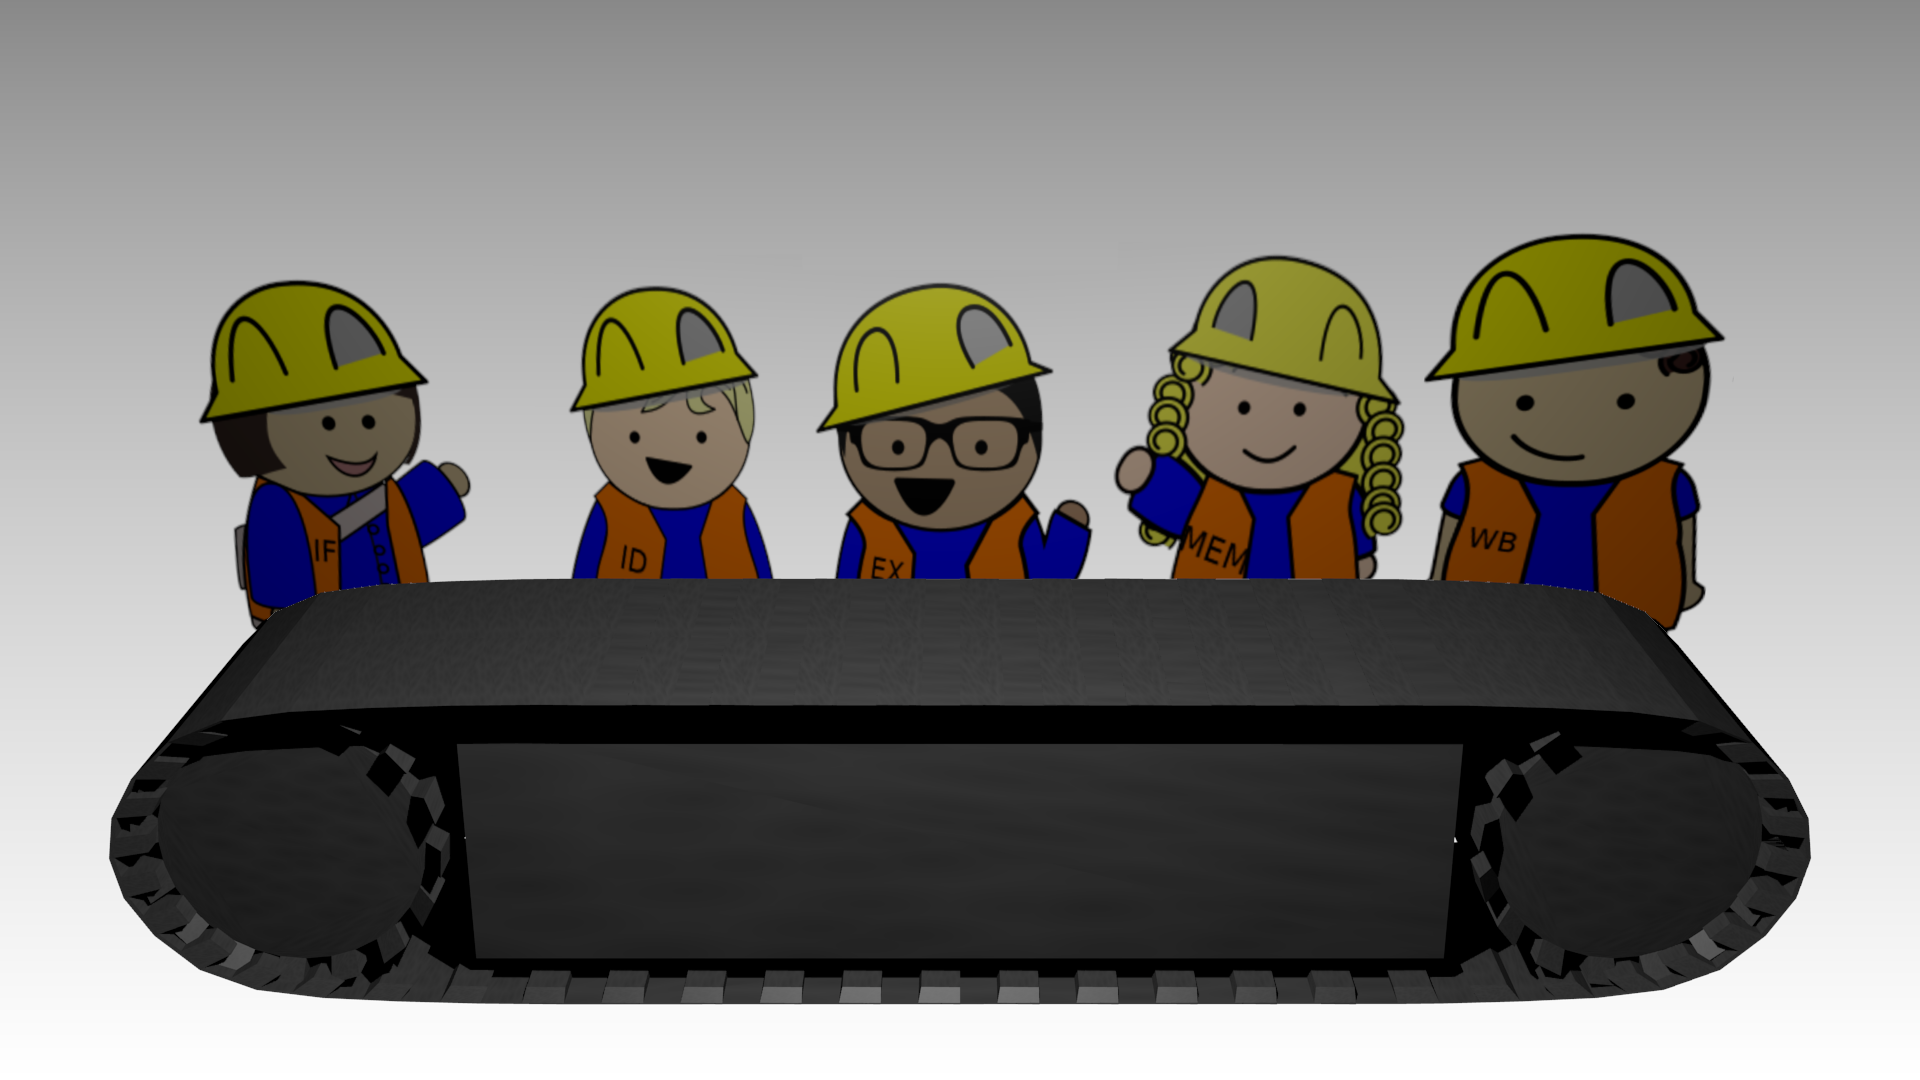
\includegraphics[width=1.0\textwidth]{final.png}}
	%FETCH
	\put(50,-12){\tiny\color{white}}
	
	%DECODE
	\put(90,-12){\tiny\color{white}}
	\put(90,-17){\tiny\color{white}}
	
	%EXECUTE
	\put(135,-12){\tiny\color{white}add t0, t0, 1}
	\put(135,-17){\tiny\color{white}t0 = 0 + 1}
	\put(135,-22){\tiny\color{white}t0 = 1}
	
	%MEMORY
	\put(185,-12){\tiny\color{white}}
	\put(185,-17){\tiny\color{white}}
	\put(185,-22){\tiny\color{white}}
	
	%WRITEBACK
	\put(225,-12){\tiny\color{white}}
	\put(225,-17){\tiny\color{white}}
	\put(225,-22){\tiny\color{white}}
	
	%REGISTERS
	\put(80,-37){\tiny\color{white}zero = 0}
	\put(80,-42){\tiny\color{white}ra = 0}
	\put(80,-47){\tiny\color{white}sp = 0}
	\put(80,-52){\tiny\color{white}pc = 12}
	\put(80,-57){\tiny\color{white}t0 = 0}
	\put(80,-62){\tiny\color{white}t1 = 0}
	
	\put(110,-37){\tiny\color{white}t2 = 0}
	\put(110,-42){\tiny\color{white}t3 = 0}
	\put(110,-47){\tiny\color{white}t4 = 0}
	\put(110,-52){\tiny\color{white}t5 = 0}
	\put(110,-57){\tiny\color{white}t6 = 0}
	\put(110,-62){\tiny\color{white}a0 = 0}
	
	\put(140,-37){\tiny\color{white}a1 = 0}
	\put(140,-42){\tiny\color{white}a2 = 0}
	\put(140,-47){\tiny\color{white}a3 = 0}
	\put(140,-52){\tiny\color{white}a4 = 0}
	\put(140,-57){\tiny\color{white}a5 = 0}
	\put(140,-62){\tiny\color{white}a6 = 0}
	
	\put(170,-37){\tiny\color{white}a7 = 0}
	\put(170,-42){\tiny\color{white}s1 = 0}
	\put(170,-47){\tiny\color{white}s2 = 0}
	\put(170,-52){\tiny\color{white}s3 = 0}
	\put(170,-57){\tiny\color{white}s4 = 0}
	\put(170,-62){\tiny\color{white}s5 = 0}
	
	\put(200,-37){\tiny\color{white}s6 = 0}
	\put(200,-42){\tiny\color{white}s7 = 0}
	\put(200,-47){\tiny\color{white}s8 = 0}
	\put(200,-52){\tiny\color{white}s9 = 0}
	\put(200,-57){\tiny\color{white}s10 = 0}
	\put(200,-62){\tiny\color{white}s11 = 0}
	
	\end{picture}
\end{frame}

\begin{frame}
	\frametitle{Memory}
	\begin{picture}(0,0)
	\put(0,-85){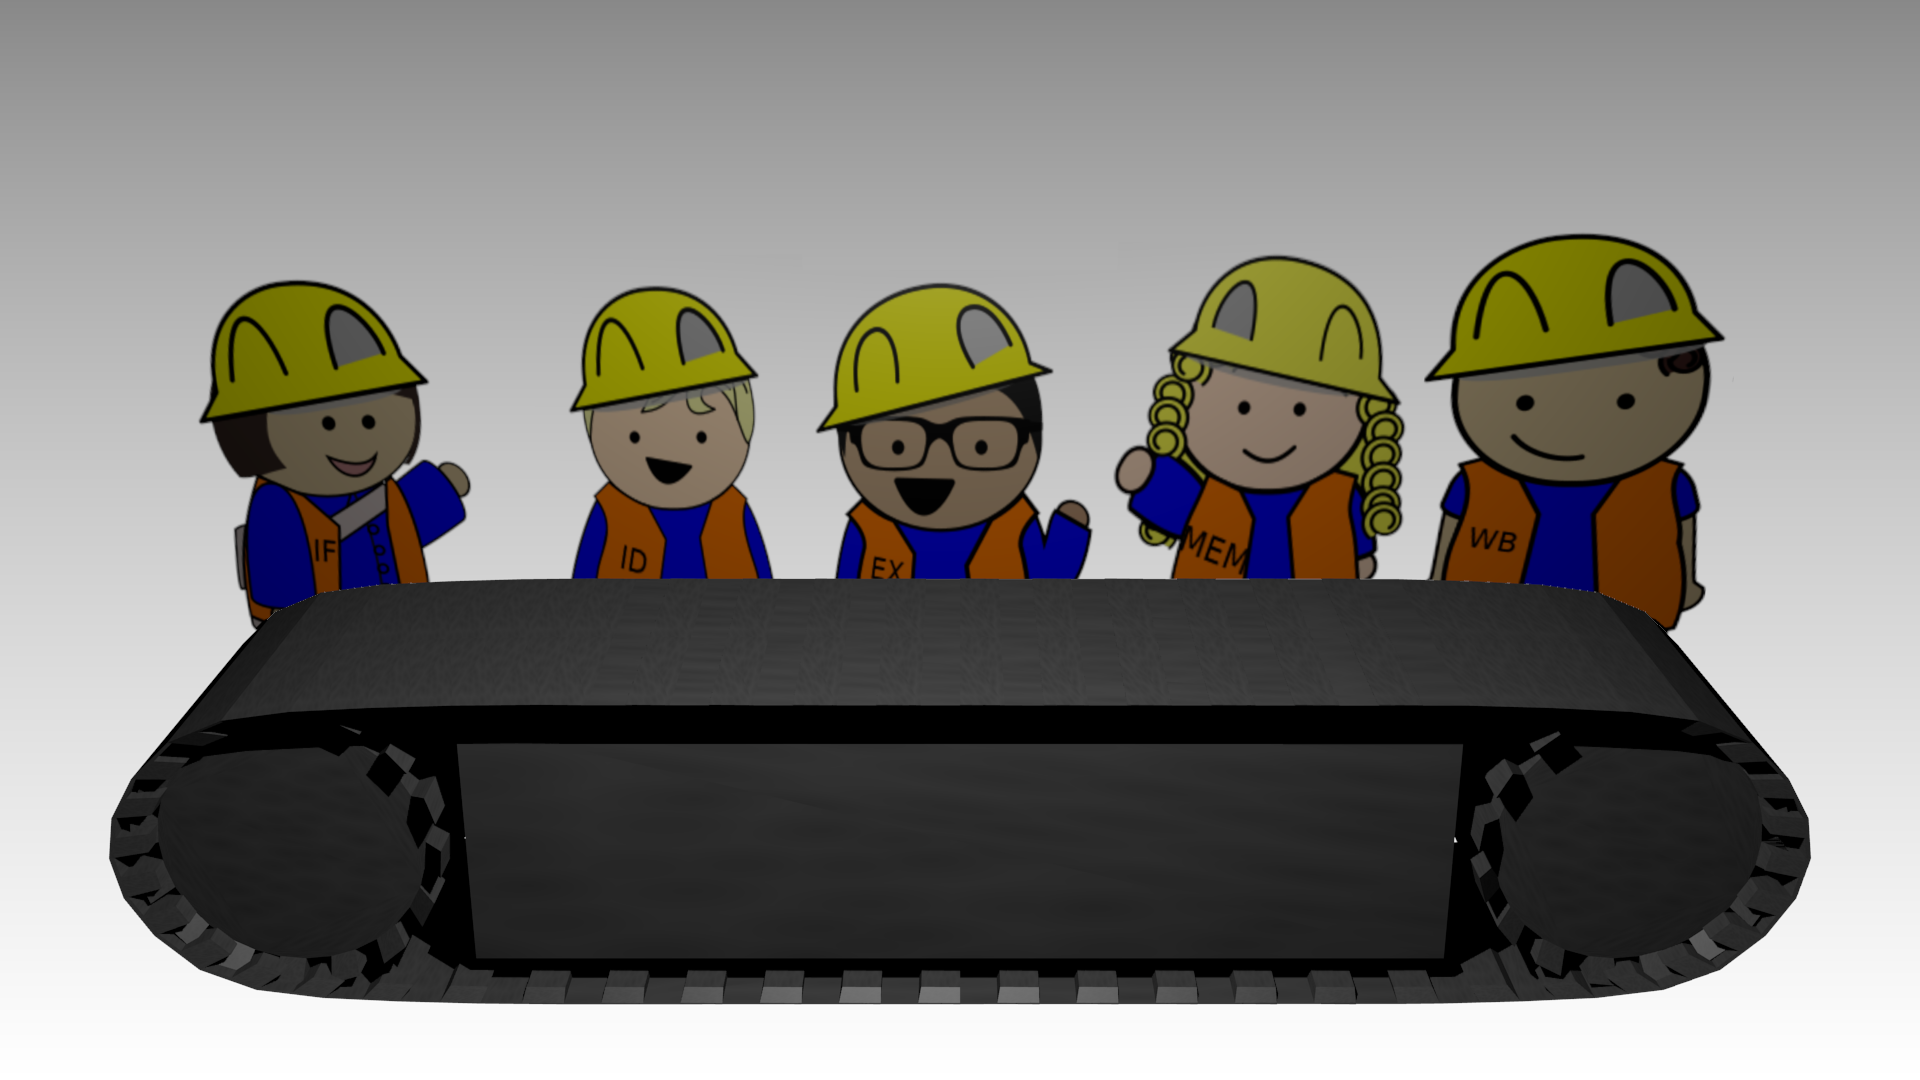
\includegraphics[width=1.0\textwidth]{final.png}}
	%FETCH
	\put(50,-12){\tiny\color{white}}
	
	%DECODE
	\put(90,-12){\tiny\color{white}}
	\put(90,-17){\tiny\color{white}}
	
	%EXECUTE
	\put(135,-12){\tiny\color{white}}
	\put(135,-17){\tiny\color{white}}
	\put(135,-22){\tiny\color{white}}
	
	%MEMORY
	\put(185,-12){\tiny\color{white}add t0, t0, 1}
	\put(185,-17){\tiny\color{white}t0 = 0 + 1}
	\put(185,-22){\tiny\color{white}t0 = 1}
	
	%WRITEBACK
	\put(225,-12){\tiny\color{white}}
	\put(225,-17){\tiny\color{white}}
	\put(225,-22){\tiny\color{white}}
	
	%REGISTERS
	\put(80,-37){\tiny\color{white}zero = 0}
	\put(80,-42){\tiny\color{white}ra = 0}
	\put(80,-47){\tiny\color{white}sp = 0}
	\put(80,-52){\tiny\color{white}pc = 16}
	\put(80,-57){\tiny\color{white}t0 = 0}
	\put(80,-62){\tiny\color{white}t1 = 0}
	
	\put(110,-37){\tiny\color{white}t2 = 0}
	\put(110,-42){\tiny\color{white}t3 = 0}
	\put(110,-47){\tiny\color{white}t4 = 0}
	\put(110,-52){\tiny\color{white}t5 = 0}
	\put(110,-57){\tiny\color{white}t6 = 0}
	\put(110,-62){\tiny\color{white}a0 = 0}
	
	\put(140,-37){\tiny\color{white}a1 = 0}
	\put(140,-42){\tiny\color{white}a2 = 0}
	\put(140,-47){\tiny\color{white}a3 = 0}
	\put(140,-52){\tiny\color{white}a4 = 0}
	\put(140,-57){\tiny\color{white}a5 = 0}
	\put(140,-62){\tiny\color{white}a6 = 0}
	
	\put(170,-37){\tiny\color{white}a7 = 0}
	\put(170,-42){\tiny\color{white}s1 = 0}
	\put(170,-47){\tiny\color{white}s2 = 0}
	\put(170,-52){\tiny\color{white}s3 = 0}
	\put(170,-57){\tiny\color{white}s4 = 0}
	\put(170,-62){\tiny\color{white}s5 = 0}
	
	\put(200,-37){\tiny\color{white}s6 = 0}
	\put(200,-42){\tiny\color{white}s7 = 0}
	\put(200,-47){\tiny\color{white}s8 = 0}
	\put(200,-52){\tiny\color{white}s9 = 0}
	\put(200,-57){\tiny\color{white}s10 = 0}
	\put(200,-62){\tiny\color{white}s11 = 0}
	
	\end{picture}
\end{frame}

\begin{frame}
	\frametitle{Writeback}
	\begin{picture}(0,0)
	\put(0,-85){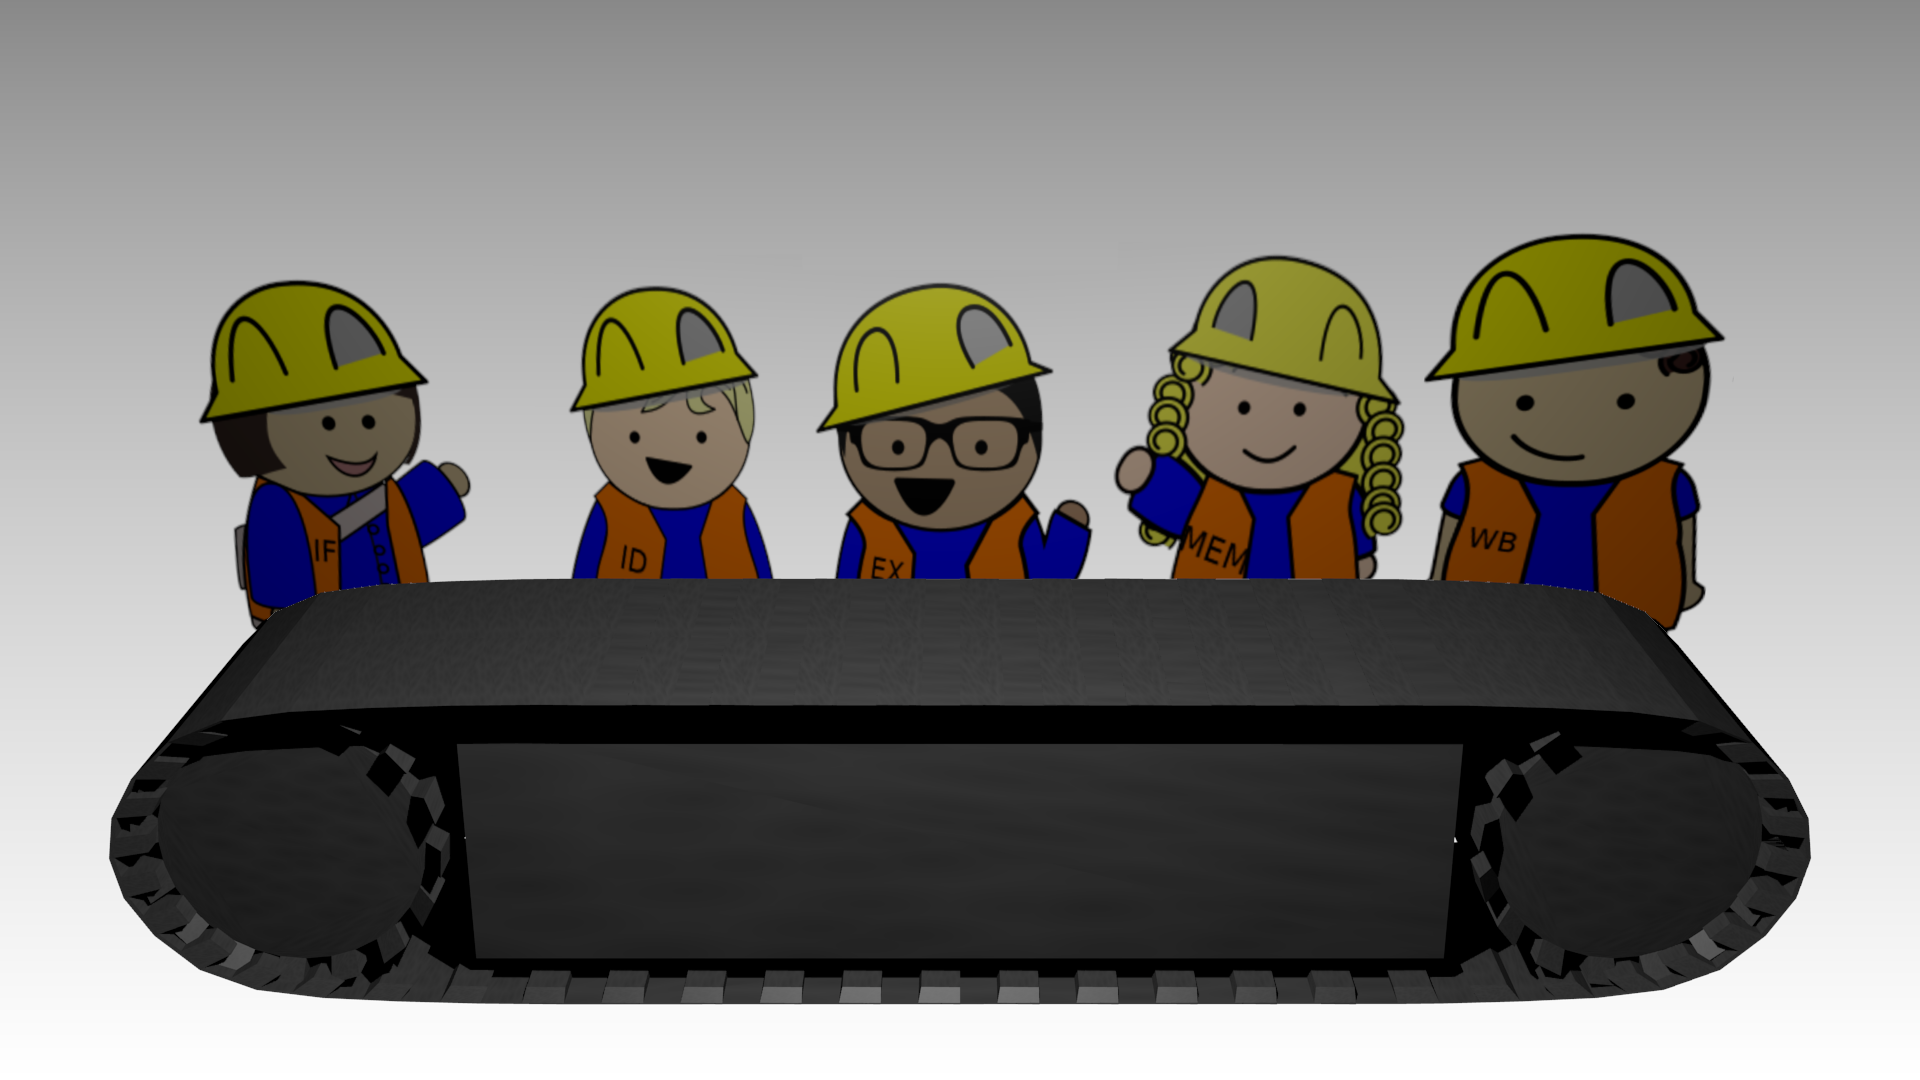
\includegraphics[width=1.0\textwidth]{final.png}}
	%FETCH
	\put(50,-12){\tiny\color{white}}
	
	%DECODE
	\put(90,-12){\tiny\color{white}}
	\put(90,-17){\tiny\color{white}}
	
	%EXECUTE
	\put(135,-12){\tiny\color{white}}
	\put(135,-17){\tiny\color{white}}
	\put(135,-22){\tiny\color{white}}
	
	%MEMORY
	\put(185,-12){\tiny\color{white}}
	\put(185,-17){\tiny\color{white}}
	\put(185,-22){\tiny\color{white}}
	
	%WRITEBACK
	\put(225,-12){\tiny\color{white}add t0, t0, 1}
	\put(225,-17){\tiny\color{white}t0 = 0 + 1}
	\put(225,-22){\tiny\color{white}t0 = 1}
	
	%REGISTERS
	\put(80,-37){\tiny\color{white}zero = 0}
	\put(80,-42){\tiny\color{white}ra = 0}
	\put(80,-47){\tiny\color{white}sp = 0}
	\put(80,-52){\tiny\color{white}pc = 20}
	\put(80,-57){\tiny\color{white}t0 = 1}
	\put(80,-62){\tiny\color{white}t1 = 0}
	
	\put(110,-37){\tiny\color{white}t2 = 0}
	\put(110,-42){\tiny\color{white}t3 = 0}
	\put(110,-47){\tiny\color{white}t4 = 0}
	\put(110,-52){\tiny\color{white}t5 = 0}
	\put(110,-57){\tiny\color{white}t6 = 0}
	\put(110,-62){\tiny\color{white}a0 = 0}
	
	\put(140,-37){\tiny\color{white}a1 = 0}
	\put(140,-42){\tiny\color{white}a2 = 0}
	\put(140,-47){\tiny\color{white}a3 = 0}
	\put(140,-52){\tiny\color{white}a4 = 0}
	\put(140,-57){\tiny\color{white}a5 = 0}
	\put(140,-62){\tiny\color{white}a6 = 0}
	
	\put(170,-37){\tiny\color{white}a7 = 0}
	\put(170,-42){\tiny\color{white}s1 = 0}
	\put(170,-47){\tiny\color{white}s2 = 0}
	\put(170,-52){\tiny\color{white}s3 = 0}
	\put(170,-57){\tiny\color{white}s4 = 0}
	\put(170,-62){\tiny\color{white}s5 = 0}
	
	\put(200,-37){\tiny\color{white}s6 = 0}
	\put(200,-42){\tiny\color{white}s7 = 0}
	\put(200,-47){\tiny\color{white}s8 = 0}
	\put(200,-52){\tiny\color{white}s9 = 0}
	\put(200,-57){\tiny\color{white}s10 = 0}
	\put(200,-62){\tiny\color{white}s11 = 0}
	
	\end{picture}
\end{frame}

\begin{frame}
	\frametitle{Pipeline Konflikt: Takt 0}
	\begin{picture}(0,0)
	\put(0,-85){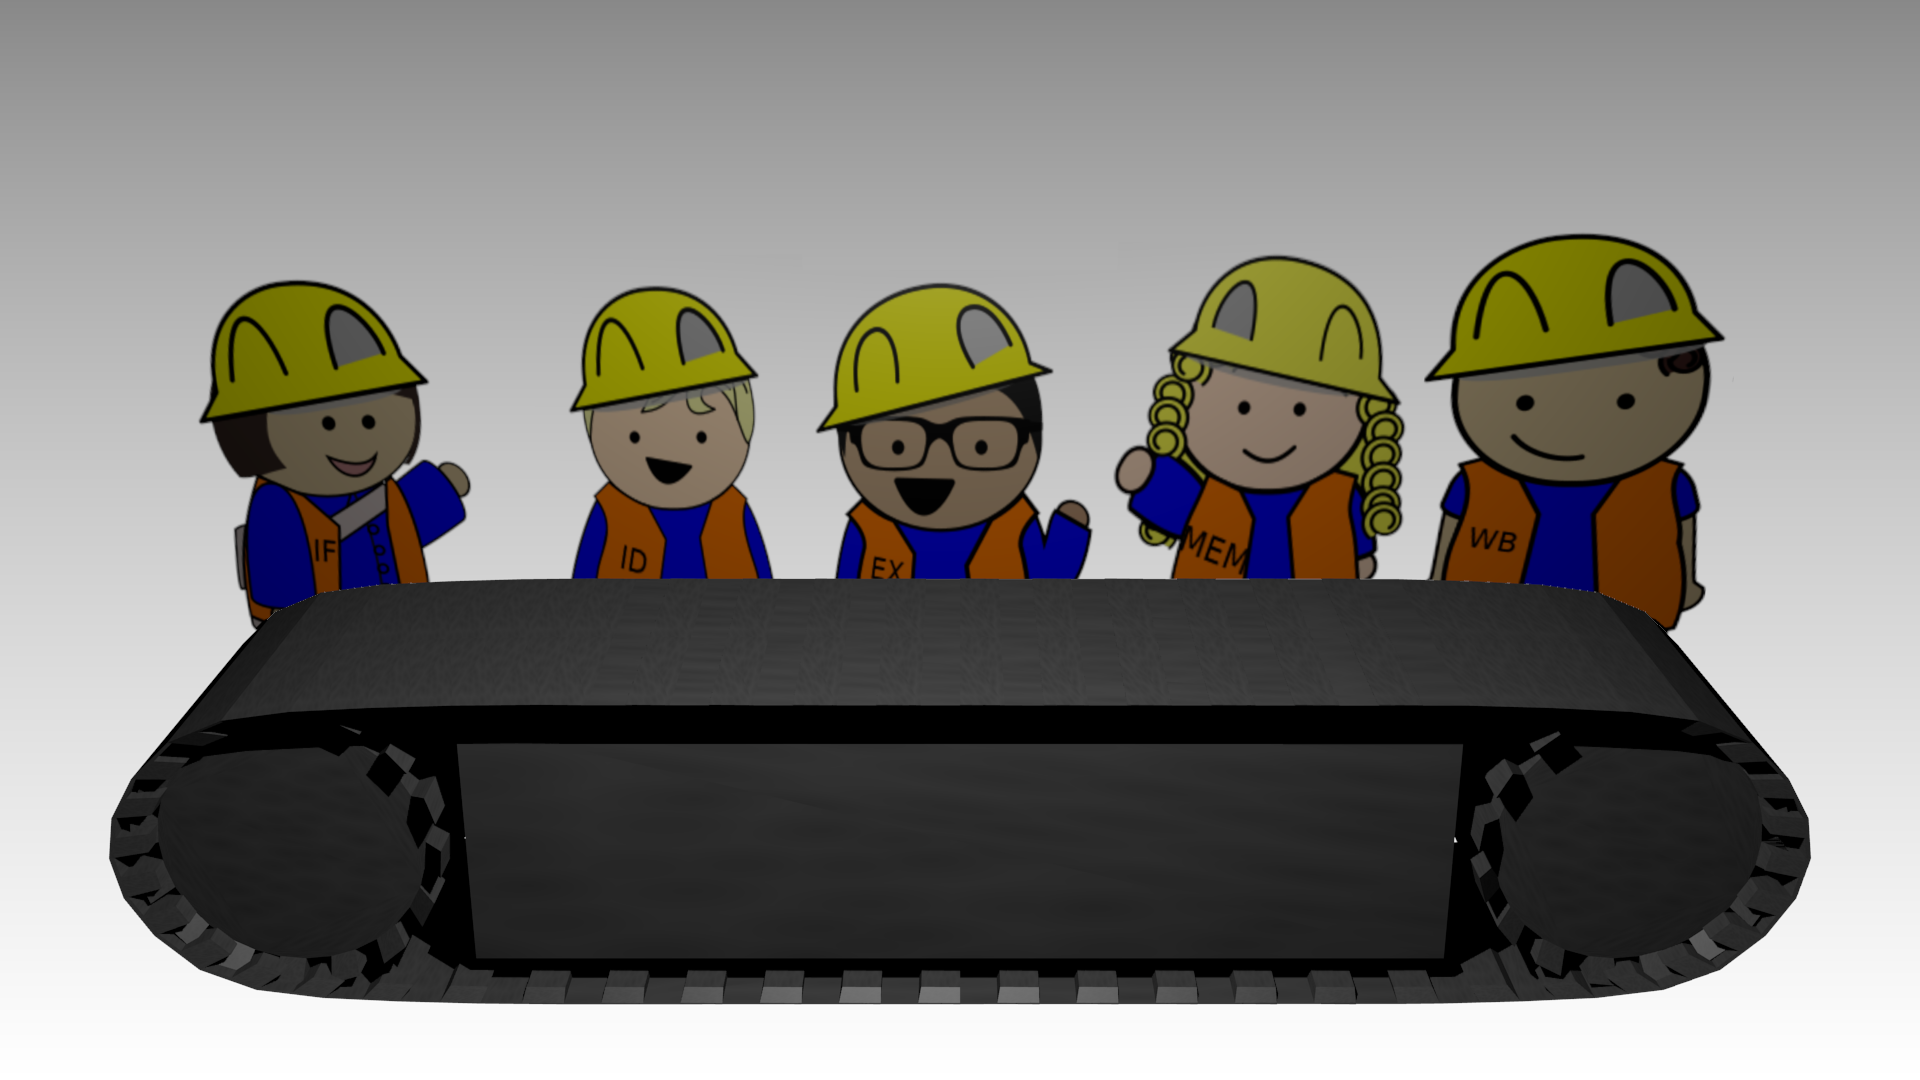
\includegraphics[width=1.0\textwidth]{final.png}}
	%FETCH
	\put(50,-12){\tiny\color{white}}
	
	%DECODE
	\put(90,-12){\tiny\color{white}}
	\put(90,-17){\tiny\color{white}}
	
	%EXECUTE
	\put(135,-12){\tiny\color{white}}
	\put(135,-17){\tiny\color{white}}
	\put(135,-22){\tiny\color{white}}
	
	%MEMORY
	\put(185,-12){\tiny\color{white}}
	\put(185,-17){\tiny\color{white}}
	\put(185,-22){\tiny\color{white}}
	
	%WRITEBACK
	\put(225,-12){\tiny\color{white}}
	\put(225,-17){\tiny\color{white}}
	\put(225,-22){\tiny\color{white}}
	
	%REGISTERS
	\put(80,-37){\tiny\color{white}zero = 0}
	\put(80,-42){\tiny\color{white}ra = 0}
	\put(80,-47){\tiny\color{white}sp = 0}
	\put(80,-52){\tiny\color{white}pc = 0}
	\put(80,-57){\tiny\color{white}t0 = 0}
	\put(80,-62){\tiny\color{white}t1 = 0}
	
	\put(110,-37){\tiny\color{white}t2 = 0}
	\put(110,-42){\tiny\color{white}t3 = 0}
	\put(110,-47){\tiny\color{white}t4 = 0}
	\put(110,-52){\tiny\color{white}t5 = 0}
	\put(110,-57){\tiny\color{white}t6 = 0}
	\put(110,-62){\tiny\color{white}a0 = 0}
	
	\put(140,-37){\tiny\color{white}a1 = 0}
	\put(140,-42){\tiny\color{white}a2 = 0}
	\put(140,-47){\tiny\color{white}a3 = 0}
	\put(140,-52){\tiny\color{white}a4 = 0}
	\put(140,-57){\tiny\color{white}a5 = 0}
	\put(140,-62){\tiny\color{white}a6 = 0}
	
	\put(170,-37){\tiny\color{white}a7 = 0}
	\put(170,-42){\tiny\color{white}s1 = 0}
	\put(170,-47){\tiny\color{white}s2 = 0}
	\put(170,-52){\tiny\color{white}s3 = 0}
	\put(170,-57){\tiny\color{white}s4 = 0}
	\put(170,-62){\tiny\color{white}s5 = 0}
	
	\put(200,-37){\tiny\color{white}s6 = 0}
	\put(200,-42){\tiny\color{white}s7 = 0}
	\put(200,-47){\tiny\color{white}s8 = 0}
	\put(200,-52){\tiny\color{white}s9 = 0}
	\put(200,-57){\tiny\color{white}s10 = 0}
	\put(200,-62){\tiny\color{white}s11 = 0}
	
	\end{picture}
\end{frame}

\begin{frame}
	\frametitle{Pipeline Konflikt: Takt 1}
	\begin{picture}(0,0)
	\put(0,-85){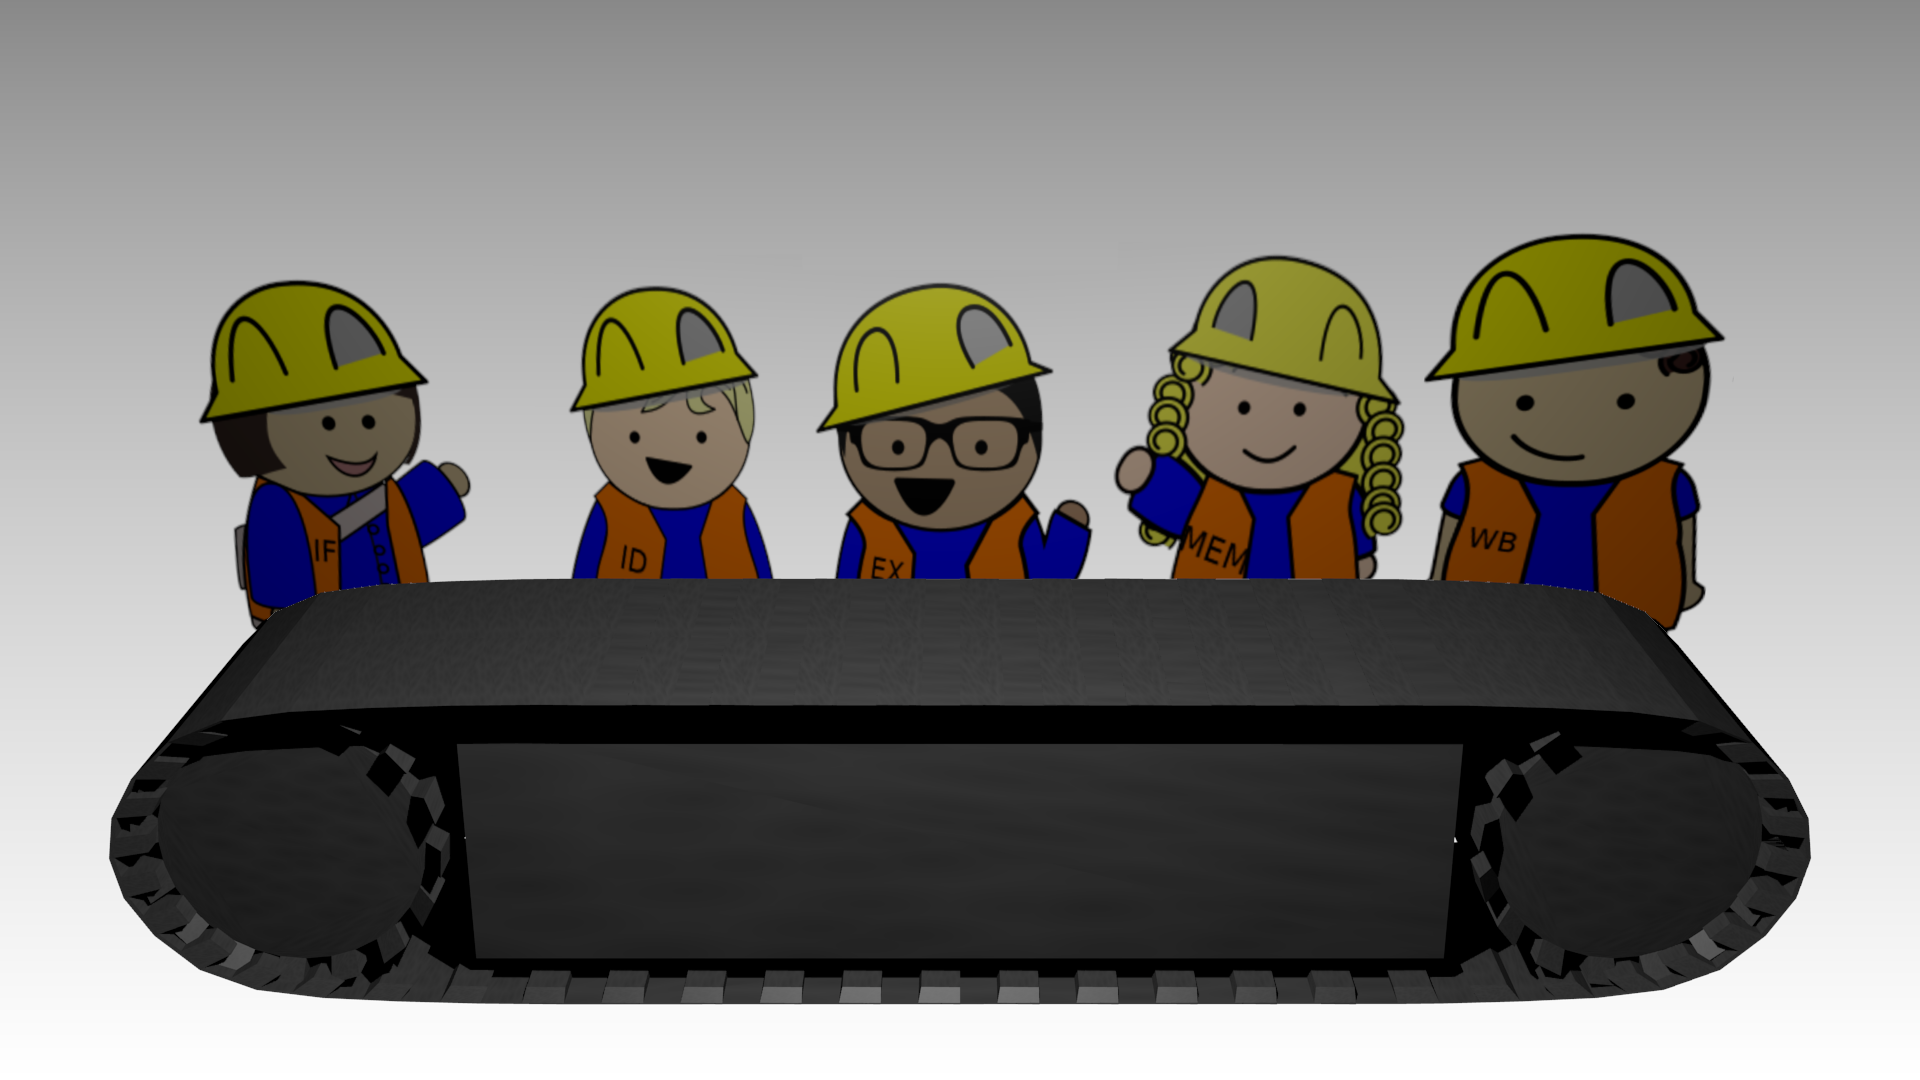
\includegraphics[width=1.0\textwidth]{final.png}}
	%FETCH
	\put(50,-12){\tiny\color{white}1:add t0, t0, 1}
	
	%DECODE
	\put(90,-12){\tiny\color{white}}
	\put(90,-17){\tiny\color{white}}
	
	%EXECUTE
	\put(135,-12){\tiny\color{white}}
	\put(135,-17){\tiny\color{white}}
	\put(135,-22){\tiny\color{white}}
	
	%MEMORY
	\put(185,-12){\tiny\color{white}}
	\put(185,-17){\tiny\color{white}}
	\put(185,-22){\tiny\color{white}}
	
	%WRITEBACK
	\put(225,-12){\tiny\color{white}}
	\put(225,-17){\tiny\color{white}}
	\put(225,-22){\tiny\color{white}}
	
	%REGISTERS
	\put(80,-37){\tiny\color{white}zero = 0}
	\put(80,-42){\tiny\color{white}ra = 0}
	\put(80,-47){\tiny\color{white}sp = 0}
	\put(80,-52){\tiny\color{white}pc = 4}
	\put(80,-57){\tiny\color{white}t0 = 0}
	\put(80,-62){\tiny\color{white}t1 = 0}
	
	\put(110,-37){\tiny\color{white}t2 = 0}
	\put(110,-42){\tiny\color{white}t3 = 0}
	\put(110,-47){\tiny\color{white}t4 = 0}
	\put(110,-52){\tiny\color{white}t5 = 0}
	\put(110,-57){\tiny\color{white}t6 = 0}
	\put(110,-62){\tiny\color{white}a0 = 0}
	
	\put(140,-37){\tiny\color{white}a1 = 0}
	\put(140,-42){\tiny\color{white}a2 = 0}
	\put(140,-47){\tiny\color{white}a3 = 0}
	\put(140,-52){\tiny\color{white}a4 = 0}
	\put(140,-57){\tiny\color{white}a5 = 0}
	\put(140,-62){\tiny\color{white}a6 = 0}
	
	\put(170,-37){\tiny\color{white}a7 = 0}
	\put(170,-42){\tiny\color{white}s1 = 0}
	\put(170,-47){\tiny\color{white}s2 = 0}
	\put(170,-52){\tiny\color{white}s3 = 0}
	\put(170,-57){\tiny\color{white}s4 = 0}
	\put(170,-62){\tiny\color{white}s5 = 0}
	
	\put(200,-37){\tiny\color{white}s6 = 0}
	\put(200,-42){\tiny\color{white}s7 = 0}
	\put(200,-47){\tiny\color{white}s8 = 0}
	\put(200,-52){\tiny\color{white}s9 = 0}
	\put(200,-57){\tiny\color{white}s10 = 0}
	\put(200,-62){\tiny\color{white}s11 = 0}
	
	\end{picture}
\end{frame}

\begin{frame}
	\frametitle{Pipeline Konflikt: Takt 2}
	\begin{picture}(0,0)
	\put(0,-85){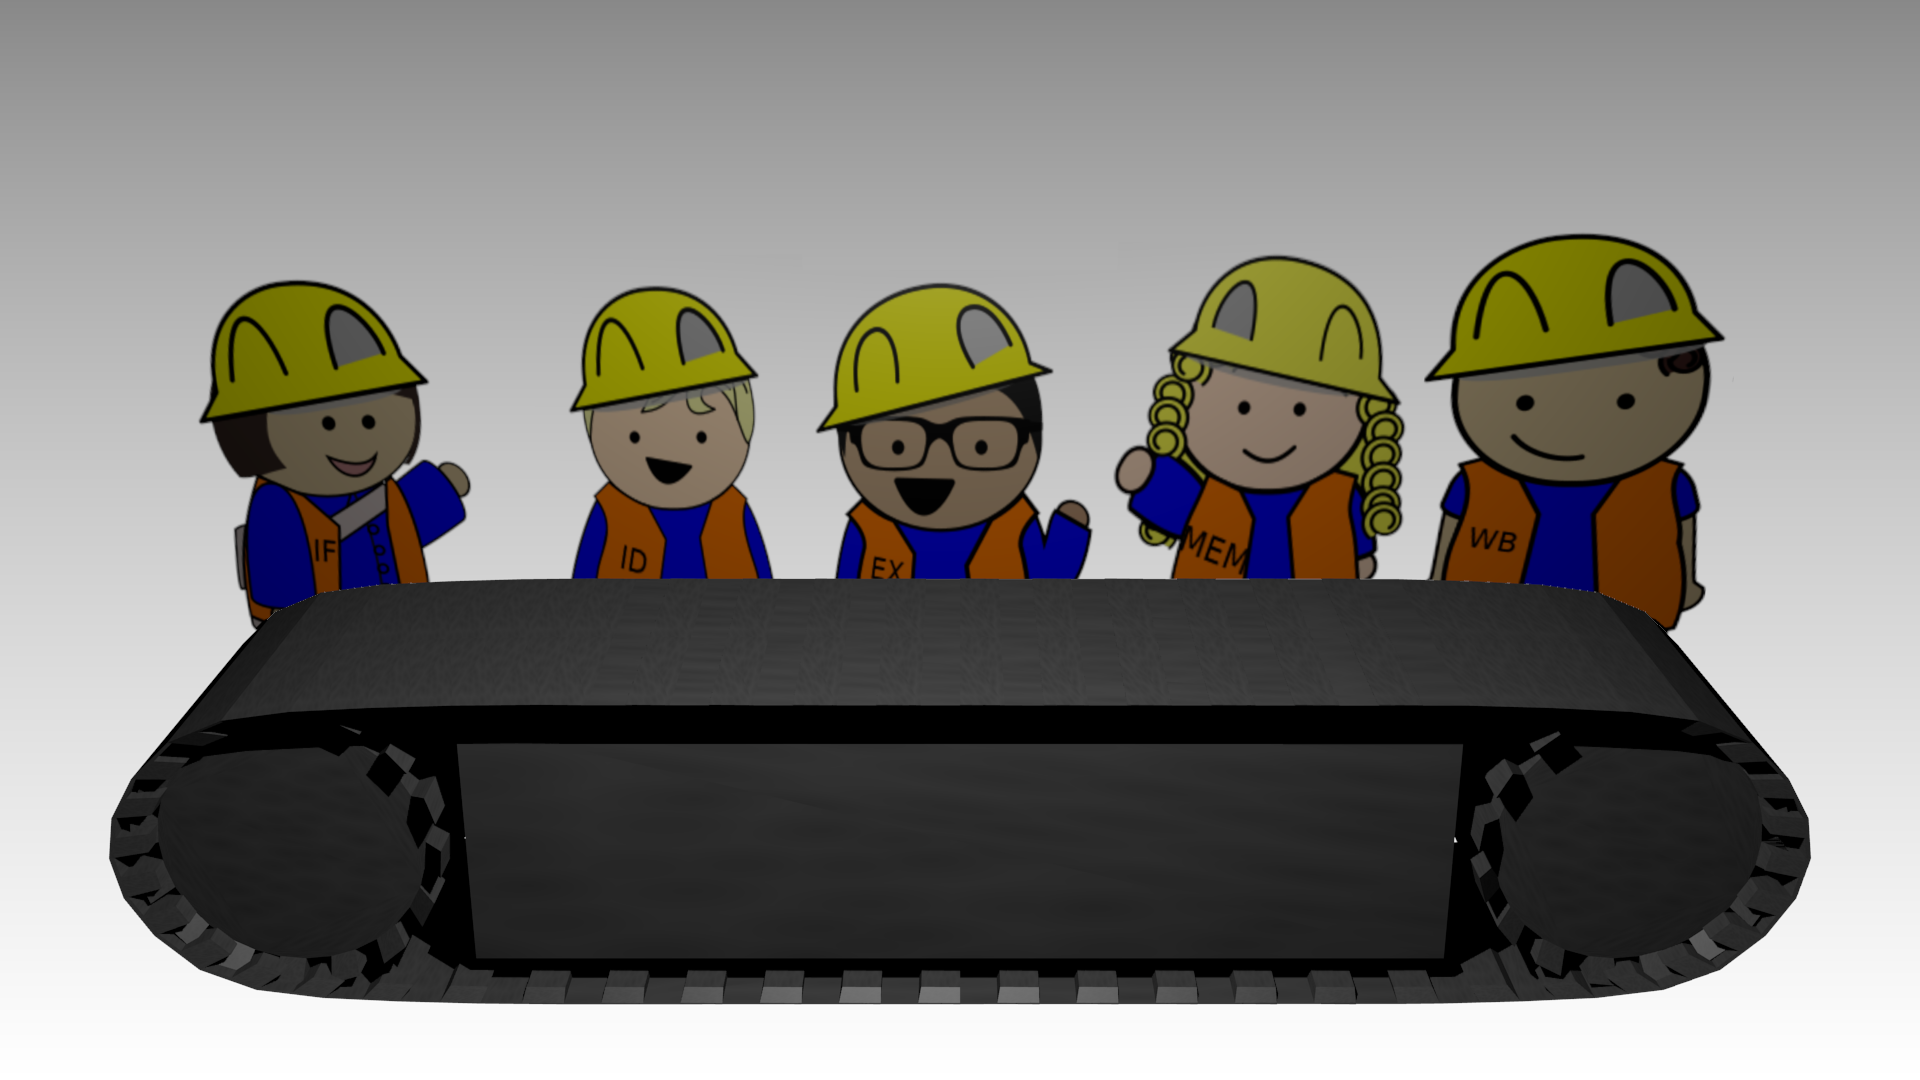
\includegraphics[width=1.0\textwidth]{final.png}}
	%FETCH
	\put(50,-12){\tiny\color{white}2:add t0, t0, 1}
	
	%DECODE
	\put(90,-12){\tiny\color{white}1:add t0, t0, 1}
	\put(90,-17){\tiny\color{white}1:t0 = 0 + 1}
	
	%EXECUTE
	\put(135,-12){\tiny\color{white}}
	\put(135,-17){\tiny\color{white}}
	\put(135,-22){\tiny\color{white}}
	
	%MEMORY
	\put(185,-12){\tiny\color{white}}
	\put(185,-17){\tiny\color{white}}
	\put(185,-22){\tiny\color{white}}
	
	%WRITEBACK
	\put(225,-12){\tiny\color{white}}
	\put(225,-17){\tiny\color{white}}
	\put(225,-22){\tiny\color{white}}
	
	%REGISTERS
	\put(80,-37){\tiny\color{white}zero = 0}
	\put(80,-42){\tiny\color{white}ra = 0}
	\put(80,-47){\tiny\color{white}sp = 0}
	\put(80,-52){\tiny\color{white}pc = 8}
	\put(80,-57){\tiny\color{white}t0 = 0}
	\put(80,-62){\tiny\color{white}t1 = 0}
	
	\put(110,-37){\tiny\color{white}t2 = 0}
	\put(110,-42){\tiny\color{white}t3 = 0}
	\put(110,-47){\tiny\color{white}t4 = 0}
	\put(110,-52){\tiny\color{white}t5 = 0}
	\put(110,-57){\tiny\color{white}t6 = 0}
	\put(110,-62){\tiny\color{white}a0 = 0}
	
	\put(140,-37){\tiny\color{white}a1 = 0}
	\put(140,-42){\tiny\color{white}a2 = 0}
	\put(140,-47){\tiny\color{white}a3 = 0}
	\put(140,-52){\tiny\color{white}a4 = 0}
	\put(140,-57){\tiny\color{white}a5 = 0}
	\put(140,-62){\tiny\color{white}a6 = 0}
	
	\put(170,-37){\tiny\color{white}a7 = 0}
	\put(170,-42){\tiny\color{white}s1 = 0}
	\put(170,-47){\tiny\color{white}s2 = 0}
	\put(170,-52){\tiny\color{white}s3 = 0}
	\put(170,-57){\tiny\color{white}s4 = 0}
	\put(170,-62){\tiny\color{white}s5 = 0}
	
	\put(200,-37){\tiny\color{white}s6 = 0}
	\put(200,-42){\tiny\color{white}s7 = 0}
	\put(200,-47){\tiny\color{white}s8 = 0}
	\put(200,-52){\tiny\color{white}s9 = 0}
	\put(200,-57){\tiny\color{white}s10 = 0}
	\put(200,-62){\tiny\color{white}s11 = 0}
	
	\end{picture}
\end{frame}

\begin{frame}
	\frametitle{Pipeline Konflikt: Takt 3}
	\begin{picture}(0,0)
	\put(0,-85){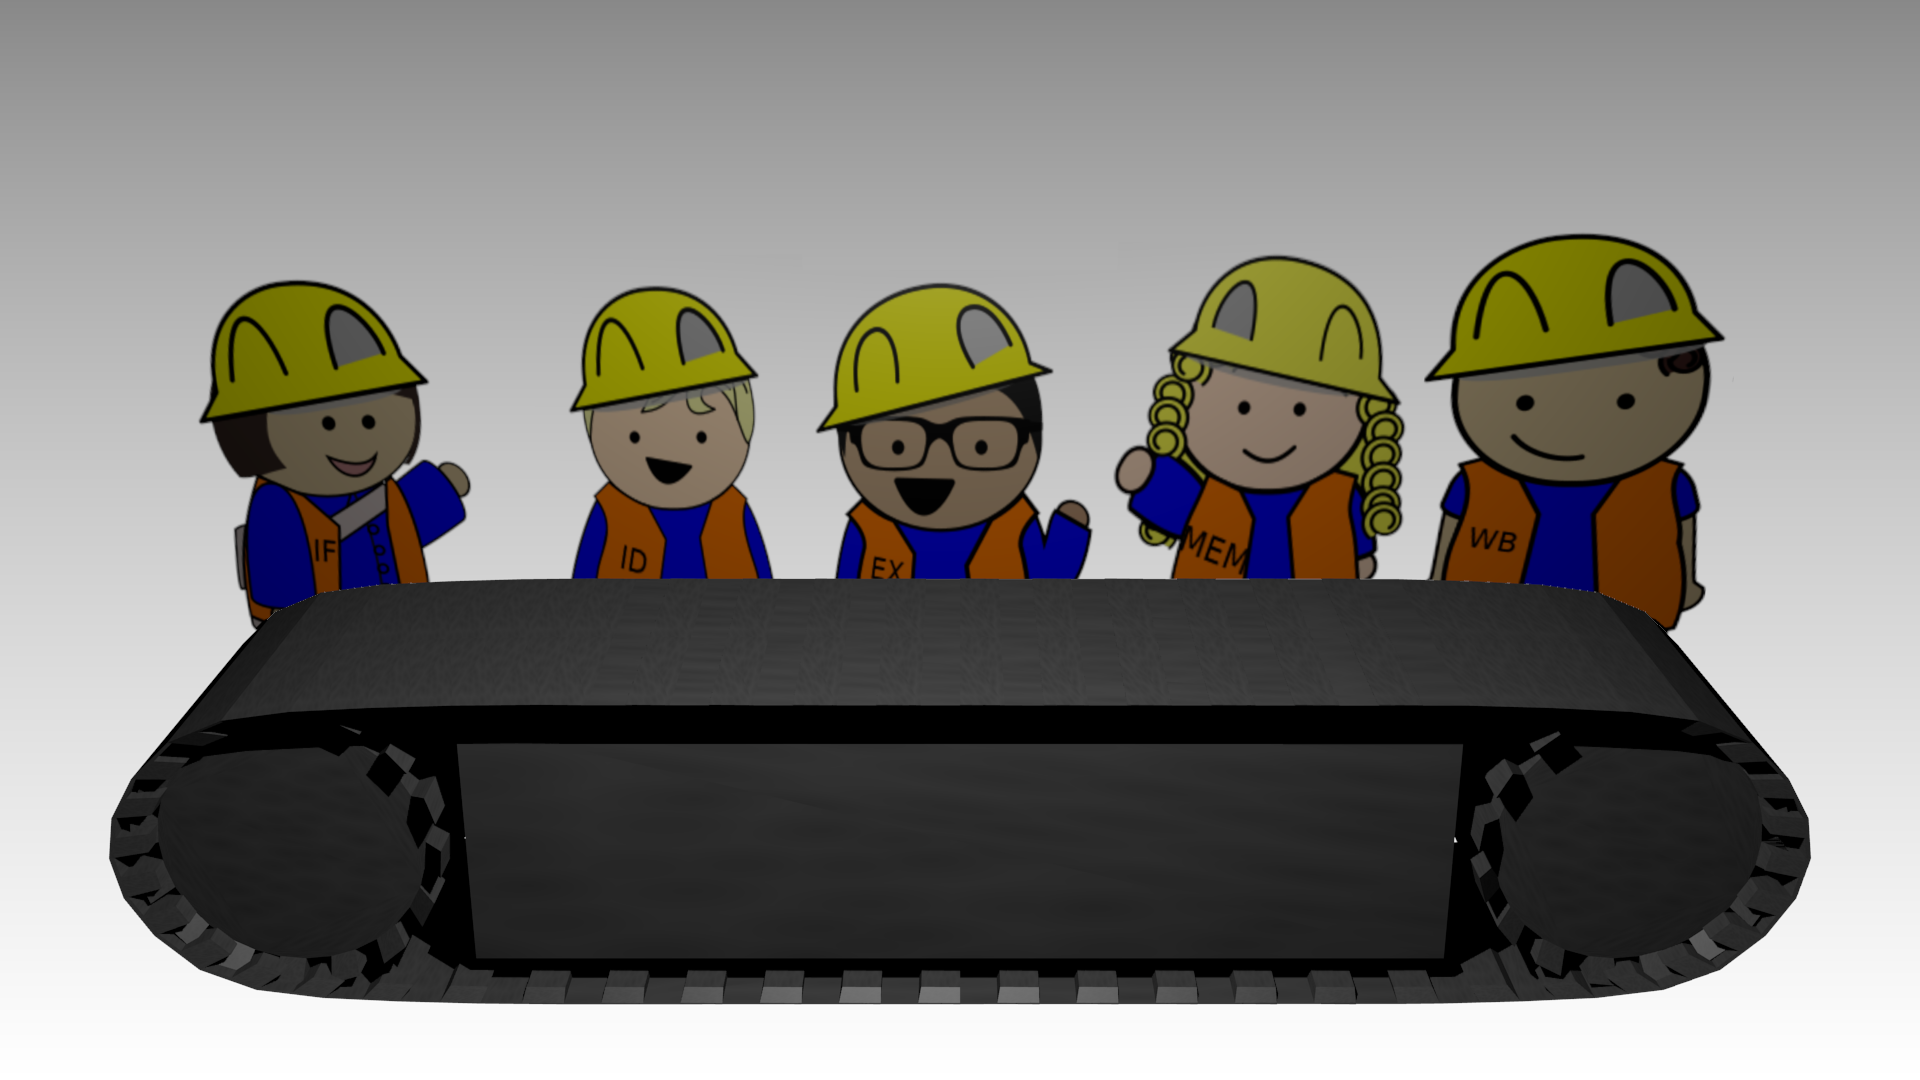
\includegraphics[width=1.0\textwidth]{final.png}}
	%FETCH
	\put(50,-12){\tiny\color{white}3:add t0, t0, 1}
	
	%DECODE
	\put(90,-12){\tiny\color{white}2:add t0, t0, 1}
	\put(90,-17){\tiny\color{white}2:t0 = 0 + 1}
	
	%EXECUTE
	\put(135,-12){\tiny\color{white}1:add t0, t0, 1}
	\put(135,-17){\tiny\color{white}1:t0 = 0 + 1}
	\put(135,-22){\tiny\color{white}1:t0 = 1}
	
	%MEMORY
	\put(185,-12){\tiny\color{white}}
	\put(185,-17){\tiny\color{white}}
	\put(185,-22){\tiny\color{white}}
	
	%WRITEBACK
	\put(225,-12){\tiny\color{white}}
	\put(225,-17){\tiny\color{white}}
	\put(225,-22){\tiny\color{white}}
	
	%REGISTERS
	\put(80,-37){\tiny\color{white}zero = 0}
	\put(80,-42){\tiny\color{white}ra = 0}
	\put(80,-47){\tiny\color{white}sp = 0}
	\put(80,-52){\tiny\color{white}pc = 12}
	\put(80,-57){\tiny\color{white}t0 = 0}
	\put(80,-62){\tiny\color{white}t1 = 0}
	
	\put(110,-37){\tiny\color{white}t2 = 0}
	\put(110,-42){\tiny\color{white}t3 = 0}
	\put(110,-47){\tiny\color{white}t4 = 0}
	\put(110,-52){\tiny\color{white}t5 = 0}
	\put(110,-57){\tiny\color{white}t6 = 0}
	\put(110,-62){\tiny\color{white}a0 = 0}
	
	\put(140,-37){\tiny\color{white}a1 = 0}
	\put(140,-42){\tiny\color{white}a2 = 0}
	\put(140,-47){\tiny\color{white}a3 = 0}
	\put(140,-52){\tiny\color{white}a4 = 0}
	\put(140,-57){\tiny\color{white}a5 = 0}
	\put(140,-62){\tiny\color{white}a6 = 0}
	
	\put(170,-37){\tiny\color{white}a7 = 0}
	\put(170,-42){\tiny\color{white}s1 = 0}
	\put(170,-47){\tiny\color{white}s2 = 0}
	\put(170,-52){\tiny\color{white}s3 = 0}
	\put(170,-57){\tiny\color{white}s4 = 0}
	\put(170,-62){\tiny\color{white}s5 = 0}
	
	\put(200,-37){\tiny\color{white}s6 = 0}
	\put(200,-42){\tiny\color{white}s7 = 0}
	\put(200,-47){\tiny\color{white}s8 = 0}
	\put(200,-52){\tiny\color{white}s9 = 0}
	\put(200,-57){\tiny\color{white}s10 = 0}
	\put(200,-62){\tiny\color{white}s11 = 0}
	
	\end{picture}
\end{frame}

\begin{frame}
	\frametitle{Pipeline Konflikt: Takt 4}
	\begin{picture}(0,0)
	\put(0,-85){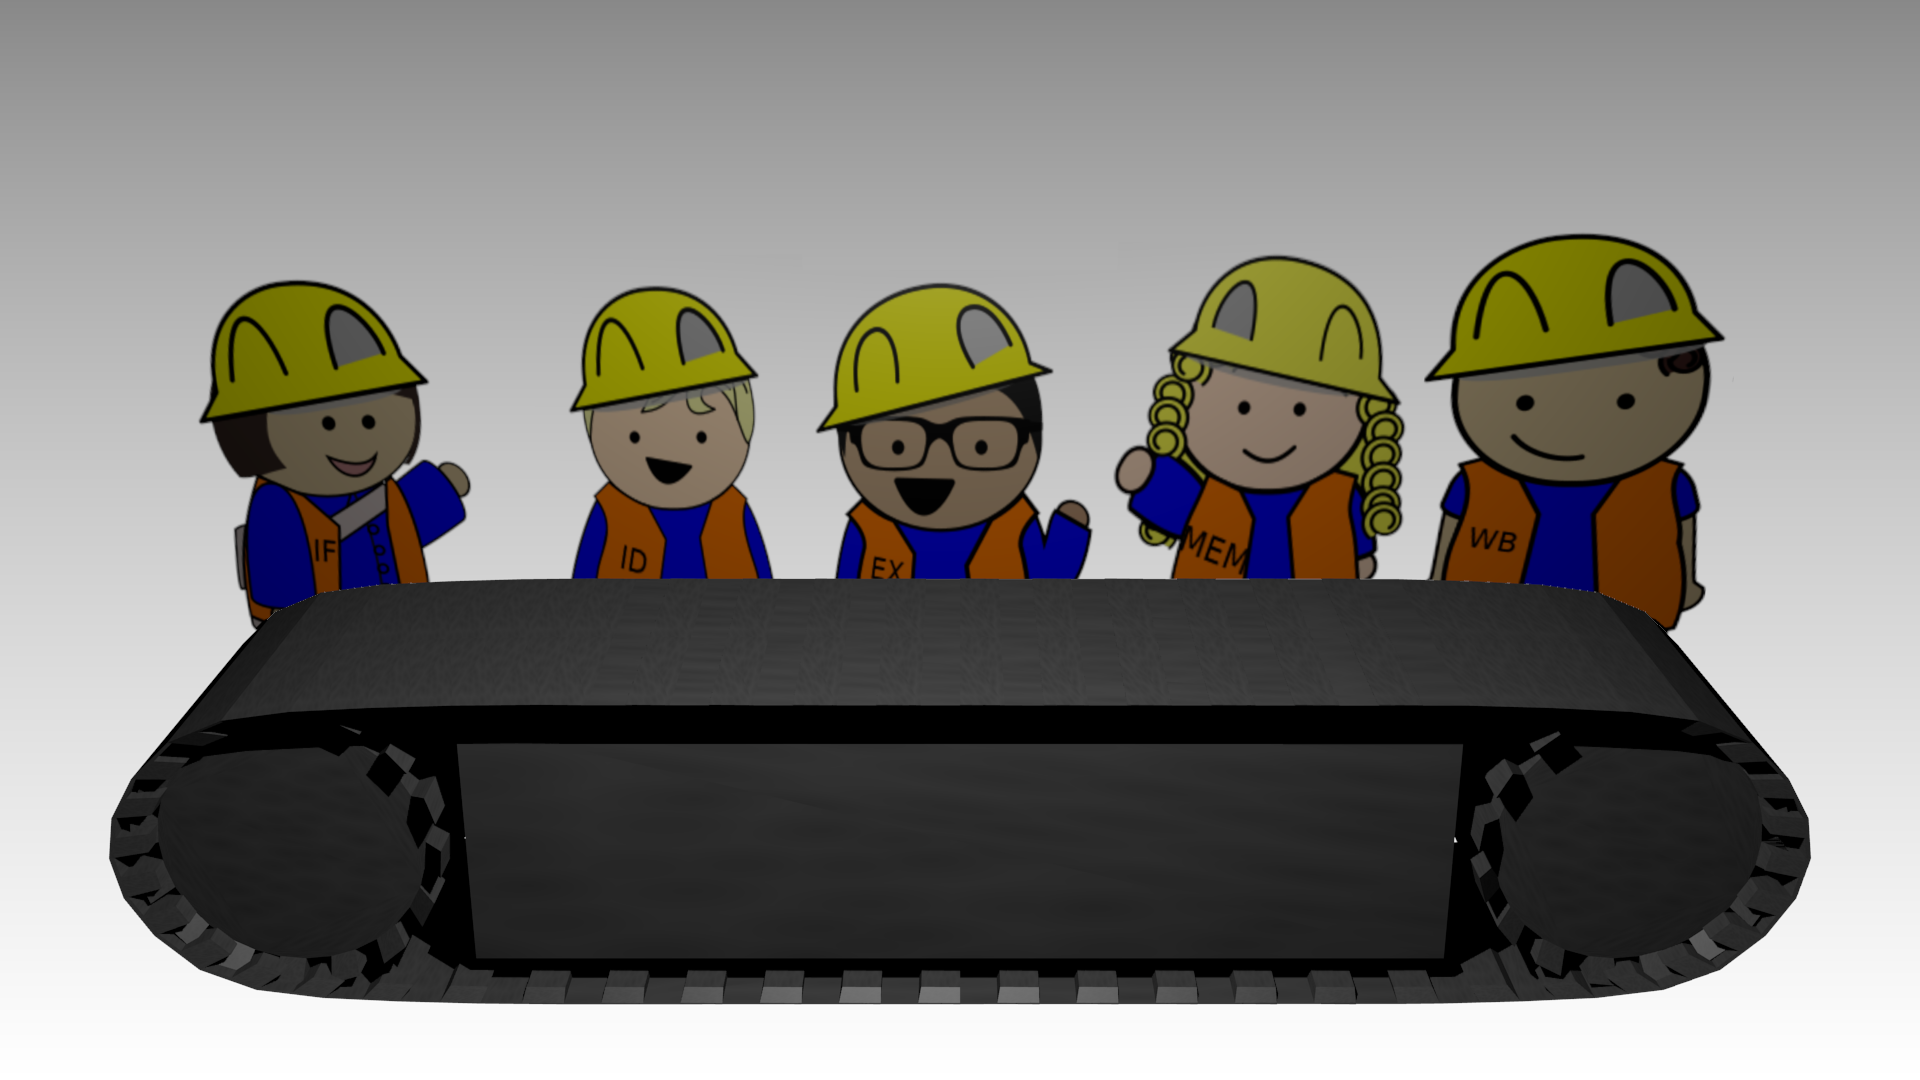
\includegraphics[width=1.0\textwidth]{final.png}}
	%FETCH
	\put(50,-12){\tiny\color{white}4:add t0, t0, 1}
	
	%DECODE
	\put(90,-12){\tiny\color{white}3:add t0, t0, 1}
	\put(90,-17){\tiny\color{white}3:t0 = 0 + 1}
	
	%EXECUTE
	\put(135,-12){\tiny\color{white}2:add t0, t0, 1}
	\put(135,-17){\tiny\color{white}2:t0 = 0 + 1}
	\put(135,-22){\tiny\color{white}2:t0 = 1}
	
	%MEMORY
	\put(185,-12){\tiny\color{white}1:add t0, t0, 1}
	\put(185,-17){\tiny\color{white}1:t0 = 0 + 1}
	\put(185,-22){\tiny\color{white}1:t0 = 1}
	
	%WRITEBACK
	\put(225,-12){\tiny\color{white}}
	\put(225,-17){\tiny\color{white}}
	\put(225,-22){\tiny\color{white}}
	
	%REGISTERS
	\put(80,-37){\tiny\color{white}zero = 0}
	\put(80,-42){\tiny\color{white}ra = 0}
	\put(80,-47){\tiny\color{white}sp = 0}
	\put(80,-52){\tiny\color{white}pc = 16}
	\put(80,-57){\tiny\color{white}t0 = 0}
	\put(80,-62){\tiny\color{white}t1 = 0}
	
	\put(110,-37){\tiny\color{white}t2 = 0}
	\put(110,-42){\tiny\color{white}t3 = 0}
	\put(110,-47){\tiny\color{white}t4 = 0}
	\put(110,-52){\tiny\color{white}t5 = 0}
	\put(110,-57){\tiny\color{white}t6 = 0}
	\put(110,-62){\tiny\color{white}a0 = 0}
	
	\put(140,-37){\tiny\color{white}a1 = 0}
	\put(140,-42){\tiny\color{white}a2 = 0}
	\put(140,-47){\tiny\color{white}a3 = 0}
	\put(140,-52){\tiny\color{white}a4 = 0}
	\put(140,-57){\tiny\color{white}a5 = 0}
	\put(140,-62){\tiny\color{white}a6 = 0}
	
	\put(170,-37){\tiny\color{white}a7 = 0}
	\put(170,-42){\tiny\color{white}s1 = 0}
	\put(170,-47){\tiny\color{white}s2 = 0}
	\put(170,-52){\tiny\color{white}s3 = 0}
	\put(170,-57){\tiny\color{white}s4 = 0}
	\put(170,-62){\tiny\color{white}s5 = 0}
	
	\put(200,-37){\tiny\color{white}s6 = 0}
	\put(200,-42){\tiny\color{white}s7 = 0}
	\put(200,-47){\tiny\color{white}s8 = 0}
	\put(200,-52){\tiny\color{white}s9 = 0}
	\put(200,-57){\tiny\color{white}s10 = 0}
	\put(200,-62){\tiny\color{white}s11 = 0}
	
	\end{picture}
\end{frame}

\begin{frame}
	\frametitle{Pipeline Konflikt: Takt 5}
	\begin{picture}(0,0)
	\put(0,-85){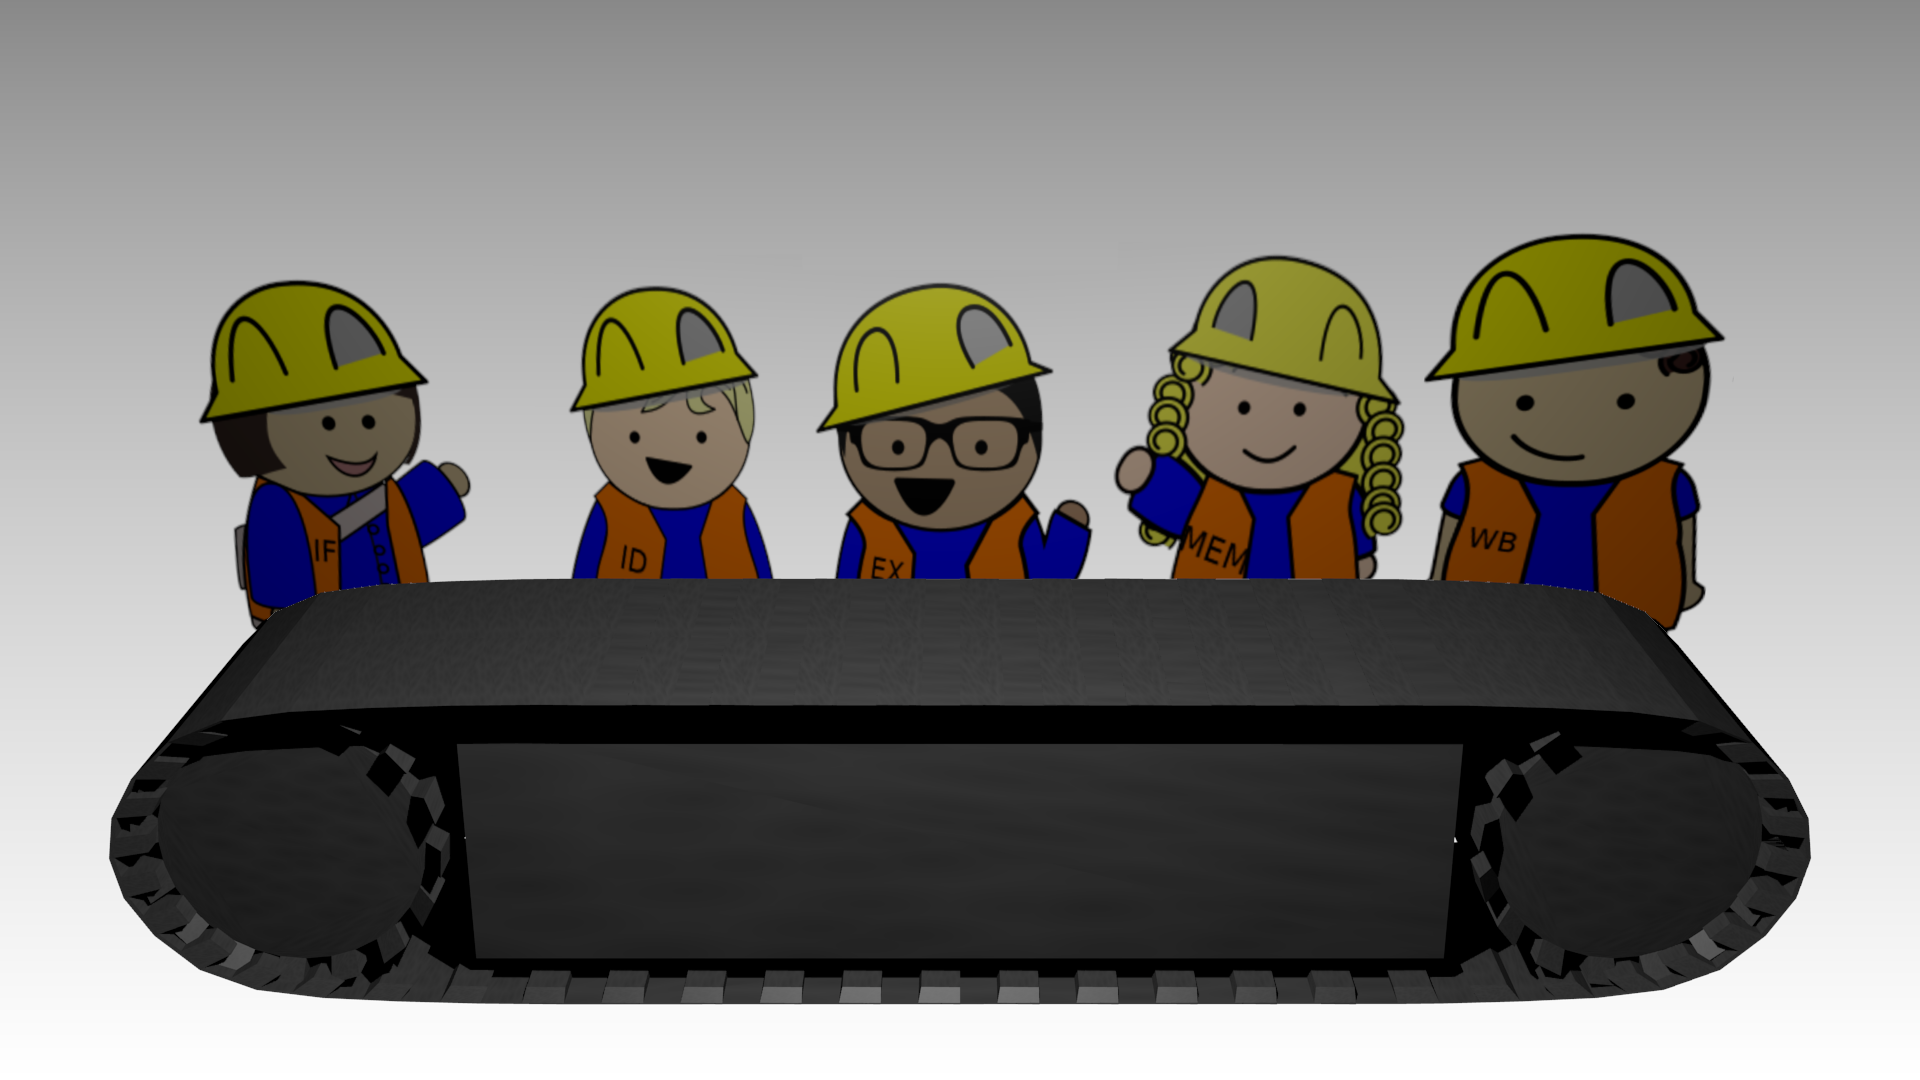
\includegraphics[width=1.0\textwidth]{final.png}}
	%FETCH
	\put(50,-12){\tiny\color{white}5:add t0, t0, 1}
	
	%DECODE
	\put(90,-12){\tiny\color{white}4:add t0, t0, 1}
	\put(90,-17){\tiny\color{white}4:t0 = 1 + 1}
	
	%EXECUTE
	\put(135,-12){\tiny\color{white}3:add t0, t0, 1}
	\put(135,-17){\tiny\color{white}3:t0 = 0 + 1}
	\put(135,-22){\tiny\color{white}3:t0 = 1}
	
	%MEMORY
	\put(185,-12){\tiny\color{white}2:add t0, t0, 1}
	\put(185,-17){\tiny\color{white}2:t0 = 0 + 1}
	\put(185,-22){\tiny\color{white}2:t0 = 1}
	
	%WRITEBACK
	\put(225,-12){\tiny\color{white}1:add t0, t0, 1}
	\put(225,-17){\tiny\color{white}1:t0 = 0 + 1}
	\put(225,-22){\tiny\color{white}1:t0 = 1}
	
	%REGISTERS
	\put(80,-37){\tiny\color{white}zero = 0}
	\put(80,-42){\tiny\color{white}ra = 0}
	\put(80,-47){\tiny\color{white}sp = 0}
	\put(80,-52){\tiny\color{white}pc = 20}
	\put(80,-57){\tiny\color{white}t0 = 1}
	\put(80,-62){\tiny\color{white}t1 = 0}
	
	\put(110,-37){\tiny\color{white}t2 = 0}
	\put(110,-42){\tiny\color{white}t3 = 0}
	\put(110,-47){\tiny\color{white}t4 = 0}
	\put(110,-52){\tiny\color{white}t5 = 0}
	\put(110,-57){\tiny\color{white}t6 = 0}
	\put(110,-62){\tiny\color{white}a0 = 0}
	
	\put(140,-37){\tiny\color{white}a1 = 0}
	\put(140,-42){\tiny\color{white}a2 = 0}
	\put(140,-47){\tiny\color{white}a3 = 0}
	\put(140,-52){\tiny\color{white}a4 = 0}
	\put(140,-57){\tiny\color{white}a5 = 0}
	\put(140,-62){\tiny\color{white}a6 = 0}
	
	\put(170,-37){\tiny\color{white}a7 = 0}
	\put(170,-42){\tiny\color{white}s1 = 0}
	\put(170,-47){\tiny\color{white}s2 = 0}
	\put(170,-52){\tiny\color{white}s3 = 0}
	\put(170,-57){\tiny\color{white}s4 = 0}
	\put(170,-62){\tiny\color{white}s5 = 0}
	
	\put(200,-37){\tiny\color{white}s6 = 0}
	\put(200,-42){\tiny\color{white}s7 = 0}
	\put(200,-47){\tiny\color{white}s8 = 0}
	\put(200,-52){\tiny\color{white}s9 = 0}
	\put(200,-57){\tiny\color{white}s10 = 0}
	\put(200,-62){\tiny\color{white}s11 = 0}
	
	\end{picture}
\end{frame}


\begin{frame}
	\frametitle{Pipeline Konflikt: Takt 6}
	\begin{picture}(0,0)
	\put(0,-85){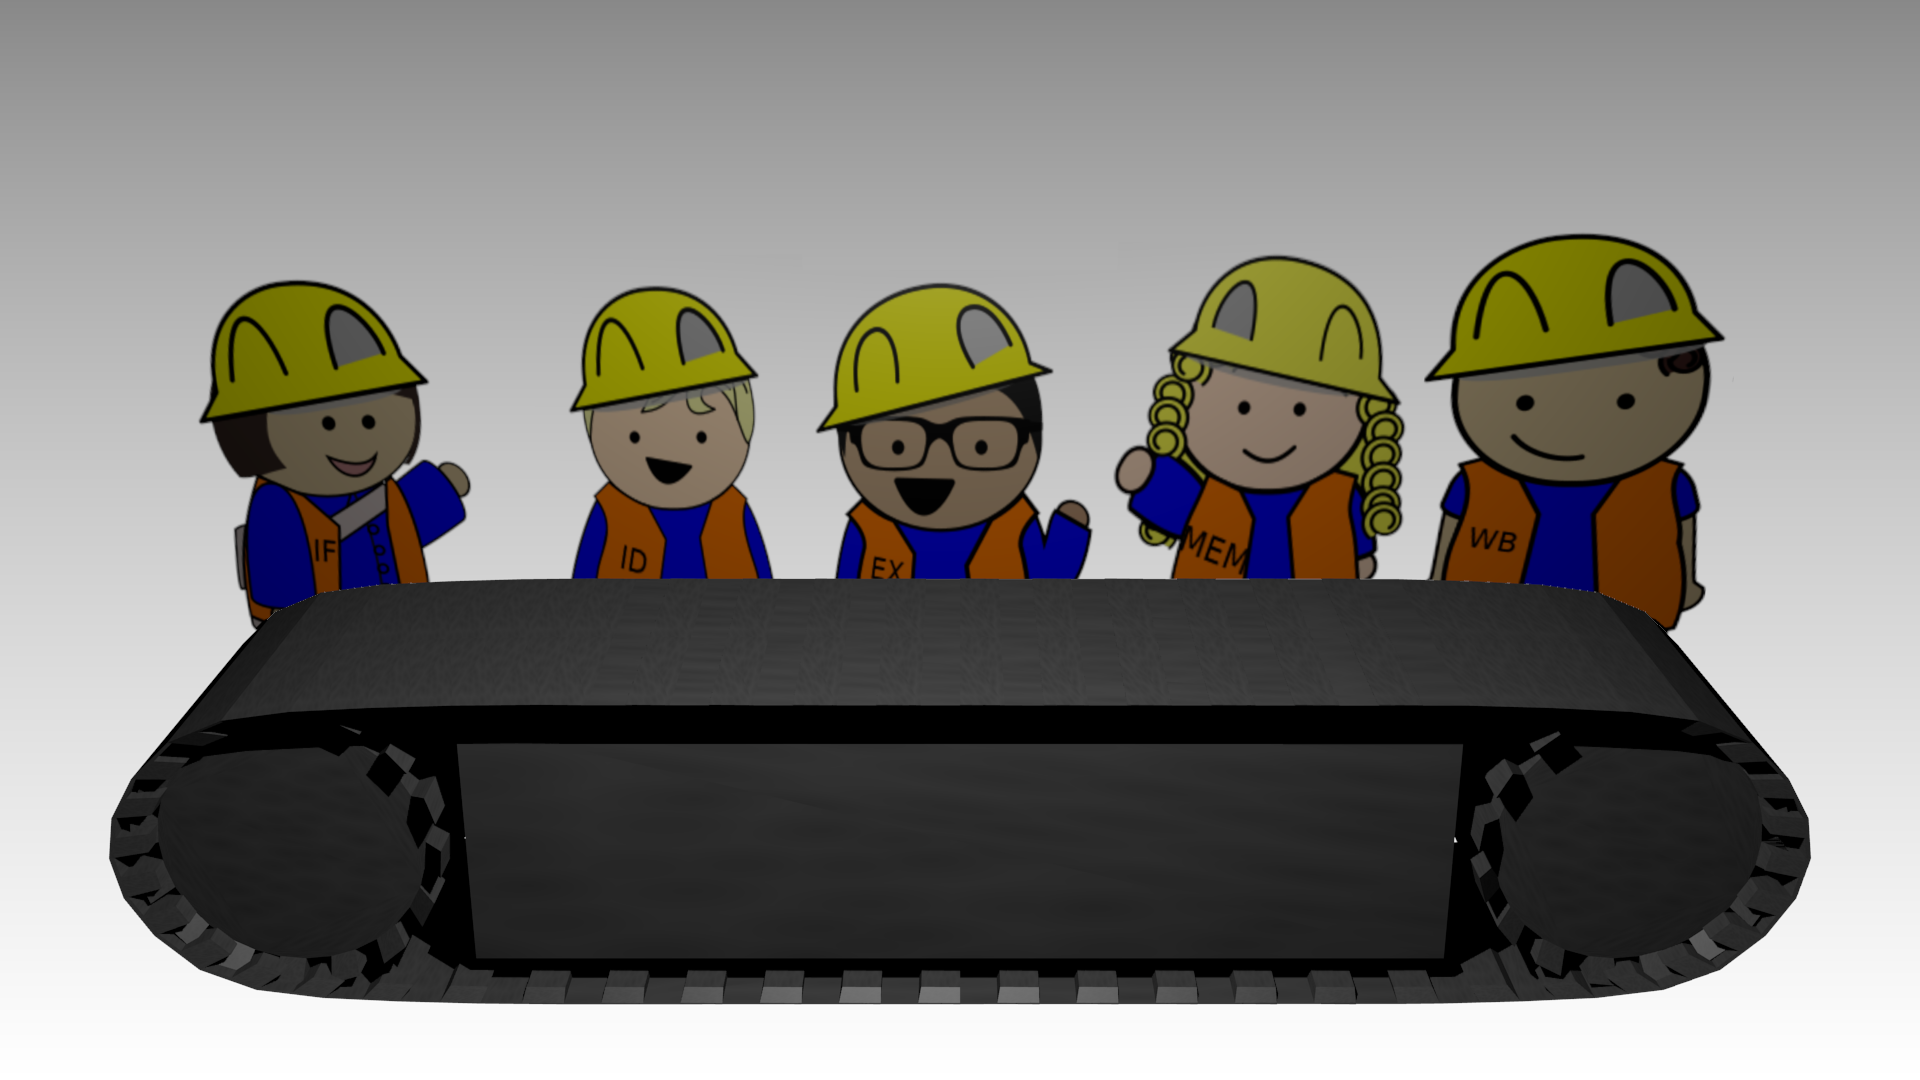
\includegraphics[width=1.0\textwidth]{final.png}}
	%FETCH
	\put(50,-12){\tiny\color{white}}
	
	%DECODE
	\put(90,-12){\tiny\color{white}5:add t0, t0, 1}
	\put(90,-17){\tiny\color{white}5:t0 = 1 + 1}
	
	%EXECUTE
	\put(135,-12){\tiny\color{white}4:add t0, t0, 1}
	\put(135,-17){\tiny\color{white}4:t0 = 1 + 1}
	\put(135,-22){\tiny\color{white}4:t0 = 2}
	
	%MEMORY
	\put(185,-12){\tiny\color{white}3:add t0, t0, 1}
	\put(185,-17){\tiny\color{white}3:t0 = 0 + 1}
	\put(185,-22){\tiny\color{white}3:t0 = 1}
	
	%WRITEBACK
	\put(225,-12){\tiny\color{white}2:add t0, t0, 1}
	\put(225,-17){\tiny\color{white}2:t0 = 0 + 1}
	\put(225,-22){\tiny\color{white}2:t0 = 1}
	
	%REGISTERS
	\put(80,-37){\tiny\color{white}zero = 0}
	\put(80,-42){\tiny\color{white}ra = 0}
	\put(80,-47){\tiny\color{white}sp = 0}
	\put(80,-52){\tiny\color{white}pc = 24}
	\put(80,-57){\tiny\color{white}t0 = 1}
	\put(80,-62){\tiny\color{white}t1 = 0}
	
	\put(110,-37){\tiny\color{white}t2 = 0}
	\put(110,-42){\tiny\color{white}t3 = 0}
	\put(110,-47){\tiny\color{white}t4 = 0}
	\put(110,-52){\tiny\color{white}t5 = 0}
	\put(110,-57){\tiny\color{white}t6 = 0}
	\put(110,-62){\tiny\color{white}a0 = 0}
	
	\put(140,-37){\tiny\color{white}a1 = 0}
	\put(140,-42){\tiny\color{white}a2 = 0}
	\put(140,-47){\tiny\color{white}a3 = 0}
	\put(140,-52){\tiny\color{white}a4 = 0}
	\put(140,-57){\tiny\color{white}a5 = 0}
	\put(140,-62){\tiny\color{white}a6 = 0}
	
	\put(170,-37){\tiny\color{white}a7 = 0}
	\put(170,-42){\tiny\color{white}s1 = 0}
	\put(170,-47){\tiny\color{white}s2 = 0}
	\put(170,-52){\tiny\color{white}s3 = 0}
	\put(170,-57){\tiny\color{white}s4 = 0}
	\put(170,-62){\tiny\color{white}s5 = 0}
	
	\put(200,-37){\tiny\color{white}s6 = 0}
	\put(200,-42){\tiny\color{white}s7 = 0}
	\put(200,-47){\tiny\color{white}s8 = 0}
	\put(200,-52){\tiny\color{white}s9 = 0}
	\put(200,-57){\tiny\color{white}s10 = 0}
	\put(200,-62){\tiny\color{white}s11 = 0}
	
	\end{picture}
\end{frame}


\begin{frame}
	\frametitle{Pipeline Konflikt: Takt 7}
	\begin{picture}(0,0)
	\put(0,-85){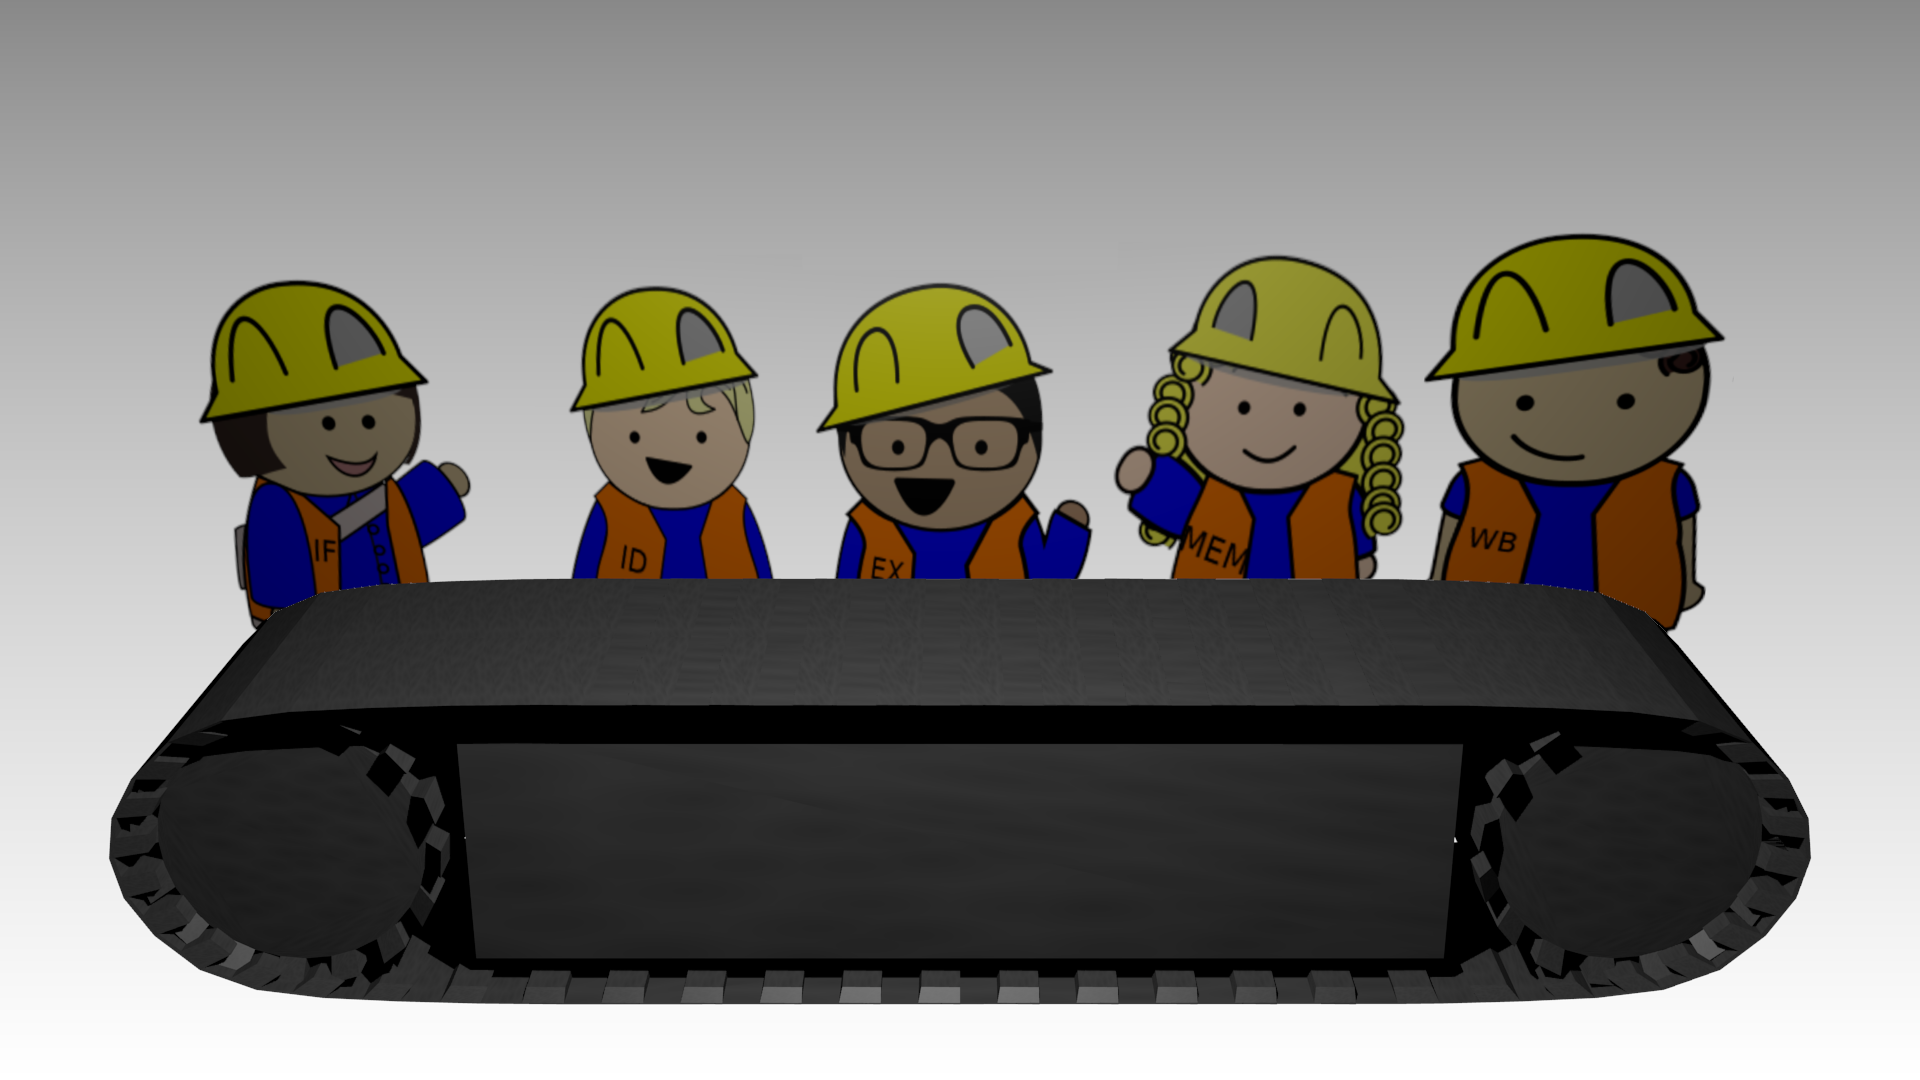
\includegraphics[width=1.0\textwidth]{final.png}}
	%FETCH
	\put(50,-12){\tiny\color{white}}
	
	%DECODE
	\put(90,-12){\tiny\color{white}}
	\put(90,-17){\tiny\color{white}}
	
	%EXECUTE
	\put(135,-12){\tiny\color{white}5:add t0, t0, 1}
	\put(135,-17){\tiny\color{white}5:t0 = 1 + 1}
	\put(135,-22){\tiny\color{white}5:t0 = 2}
	
	%MEMORY
	\put(185,-12){\tiny\color{white}4:add t0, t0, 1}
	\put(185,-17){\tiny\color{white}4:t0 = 1 + 1}
	\put(185,-22){\tiny\color{white}4:t0 = 2}
	
	%WRITEBACK
	\put(225,-12){\tiny\color{white}3:add t0, t0, 1}
	\put(225,-17){\tiny\color{white}3:t0 = 0 + 1}
	\put(225,-22){\tiny\color{white}3:t0 = 1}
	
	%REGISTERS
	\put(80,-37){\tiny\color{white}zero = 0}
	\put(80,-42){\tiny\color{white}ra = 0}
	\put(80,-47){\tiny\color{white}sp = 0}
	\put(80,-52){\tiny\color{white}pc = 28}
	\put(80,-57){\tiny\color{white}t0 = 1}
	\put(80,-62){\tiny\color{white}t1 = 0}
	
	\put(110,-37){\tiny\color{white}t2 = 0}
	\put(110,-42){\tiny\color{white}t3 = 0}
	\put(110,-47){\tiny\color{white}t4 = 0}
	\put(110,-52){\tiny\color{white}t5 = 0}
	\put(110,-57){\tiny\color{white}t6 = 0}
	\put(110,-62){\tiny\color{white}a0 = 0}
	
	\put(140,-37){\tiny\color{white}a1 = 0}
	\put(140,-42){\tiny\color{white}a2 = 0}
	\put(140,-47){\tiny\color{white}a3 = 0}
	\put(140,-52){\tiny\color{white}a4 = 0}
	\put(140,-57){\tiny\color{white}a5 = 0}
	\put(140,-62){\tiny\color{white}a6 = 0}
	
	\put(170,-37){\tiny\color{white}a7 = 0}
	\put(170,-42){\tiny\color{white}s1 = 0}
	\put(170,-47){\tiny\color{white}s2 = 0}
	\put(170,-52){\tiny\color{white}s3 = 0}
	\put(170,-57){\tiny\color{white}s4 = 0}
	\put(170,-62){\tiny\color{white}s5 = 0}
	
	\put(200,-37){\tiny\color{white}s6 = 0}
	\put(200,-42){\tiny\color{white}s7 = 0}
	\put(200,-47){\tiny\color{white}s8 = 0}
	\put(200,-52){\tiny\color{white}s9 = 0}
	\put(200,-57){\tiny\color{white}s10 = 0}
	\put(200,-62){\tiny\color{white}s11 = 0}
	
	\end{picture}
\end{frame}


\begin{frame}
	\frametitle{Pipeline Konflikt: Takt 8}
	\begin{picture}(0,0)
	\put(0,-85){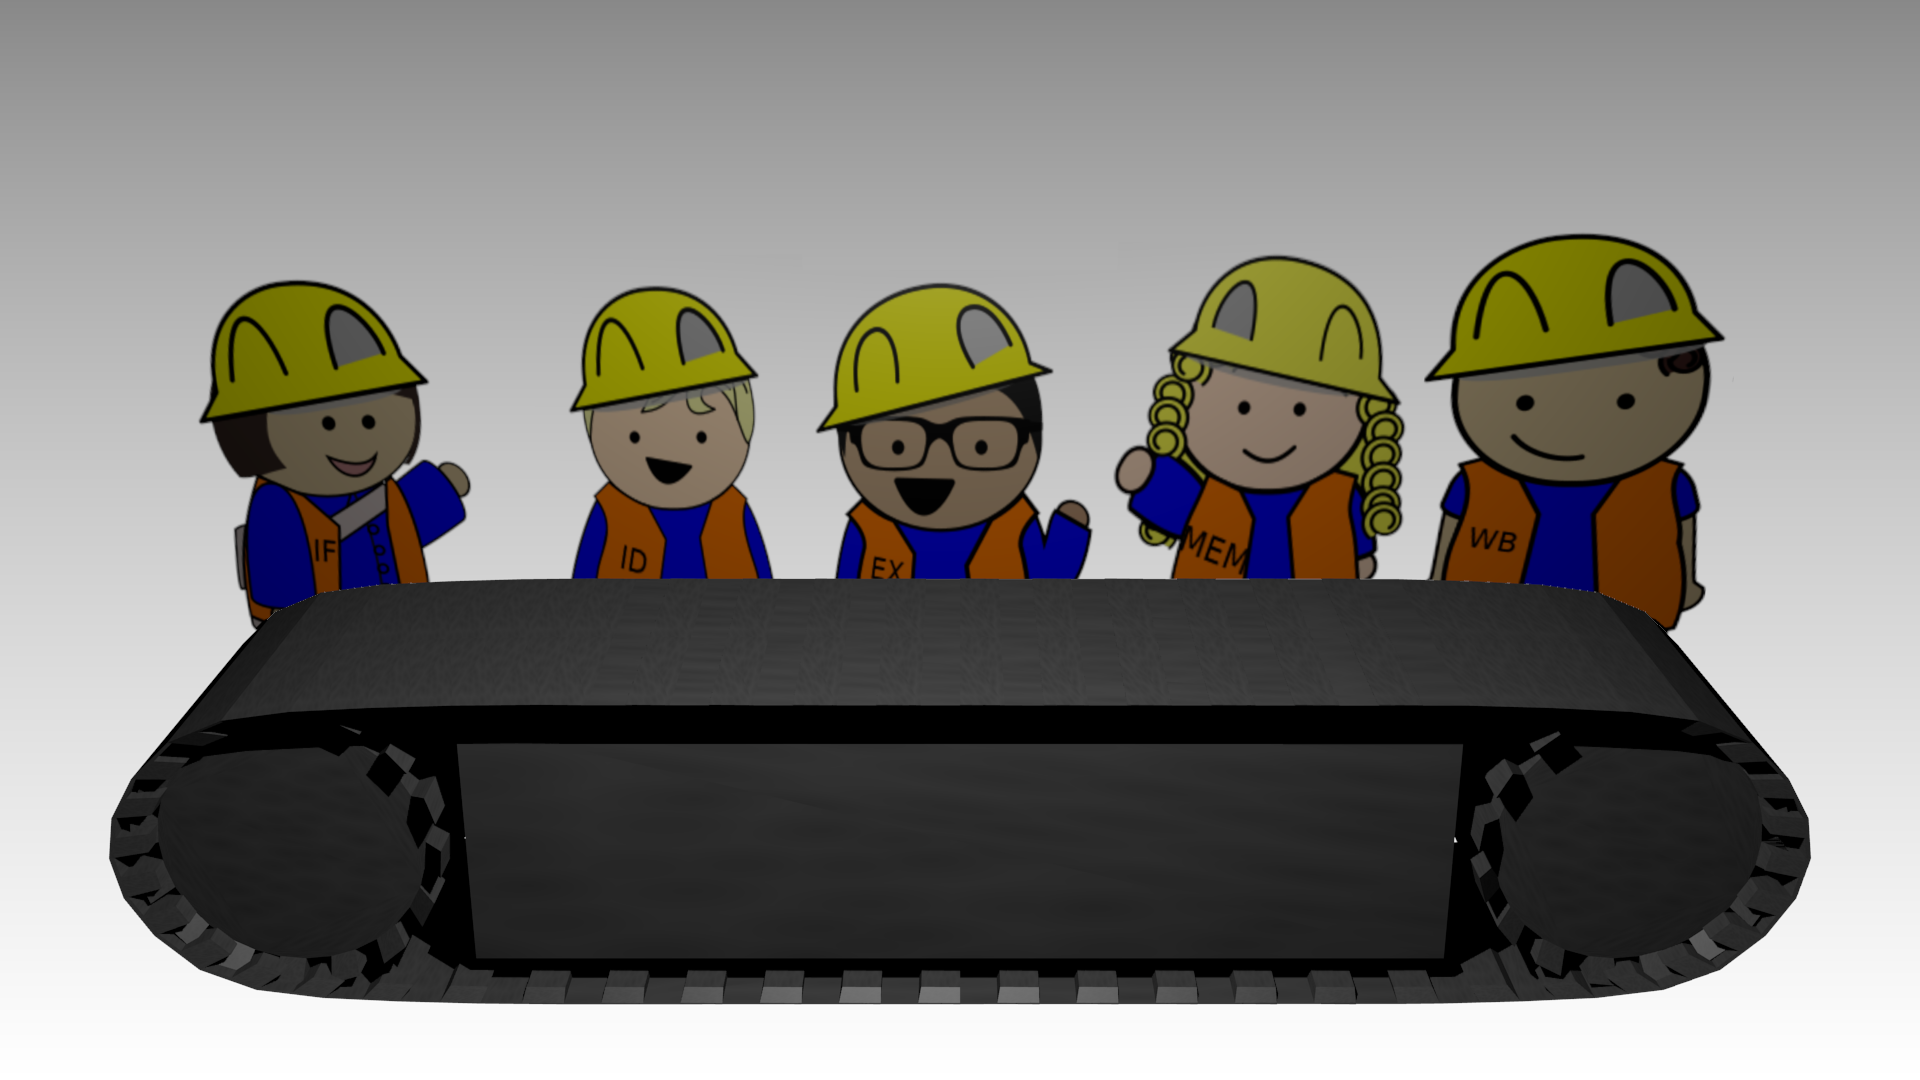
\includegraphics[width=1.0\textwidth]{final.png}}
	%FETCH
	\put(50,-12){\tiny\color{white}}
	
	%DECODE
	\put(90,-12){\tiny\color{white}}
	\put(90,-17){\tiny\color{white}}
	
	%EXECUTE
	\put(135,-12){\tiny\color{white}}
	\put(135,-17){\tiny\color{white}}
	\put(135,-22){\tiny\color{white}}
	
	%MEMORY
	\put(185,-12){\tiny\color{white}5:add t0, t0, 1}
	\put(185,-17){\tiny\color{white}5:t0 = 1 + 1}
	\put(185,-22){\tiny\color{white}5:t0 = 2}
	
	%WRITEBACK
	\put(225,-12){\tiny\color{white}4:add t0, t0, 1}
	\put(225,-17){\tiny\color{white}4:t0 = 1 + 1}
	\put(225,-22){\tiny\color{white}4:t0 = 2}
	
	%REGISTERS
	\put(80,-37){\tiny\color{white}zero = 0}
	\put(80,-42){\tiny\color{white}ra = 0}
	\put(80,-47){\tiny\color{white}sp = 0}
	\put(80,-52){\tiny\color{white}pc = 32}
	\put(80,-57){\tiny\color{white}t0 = 2}
	\put(80,-62){\tiny\color{white}t1 = 0}
	
	\put(110,-37){\tiny\color{white}t2 = 0}
	\put(110,-42){\tiny\color{white}t3 = 0}
	\put(110,-47){\tiny\color{white}t4 = 0}
	\put(110,-52){\tiny\color{white}t5 = 0}
	\put(110,-57){\tiny\color{white}t6 = 0}
	\put(110,-62){\tiny\color{white}a0 = 0}
	
	\put(140,-37){\tiny\color{white}a1 = 0}
	\put(140,-42){\tiny\color{white}a2 = 0}
	\put(140,-47){\tiny\color{white}a3 = 0}
	\put(140,-52){\tiny\color{white}a4 = 0}
	\put(140,-57){\tiny\color{white}a5 = 0}
	\put(140,-62){\tiny\color{white}a6 = 0}
	
	\put(170,-37){\tiny\color{white}a7 = 0}
	\put(170,-42){\tiny\color{white}s1 = 0}
	\put(170,-47){\tiny\color{white}s2 = 0}
	\put(170,-52){\tiny\color{white}s3 = 0}
	\put(170,-57){\tiny\color{white}s4 = 0}
	\put(170,-62){\tiny\color{white}s5 = 0}
	
	\put(200,-37){\tiny\color{white}s6 = 0}
	\put(200,-42){\tiny\color{white}s7 = 0}
	\put(200,-47){\tiny\color{white}s8 = 0}
	\put(200,-52){\tiny\color{white}s9 = 0}
	\put(200,-57){\tiny\color{white}s10 = 0}
	\put(200,-62){\tiny\color{white}s11 = 0}
	
	\end{picture}
\end{frame}

\begin{frame}
	\frametitle{Pipeline Konflikt: Takt 9}
	\begin{picture}(0,0)
	\put(0,-85){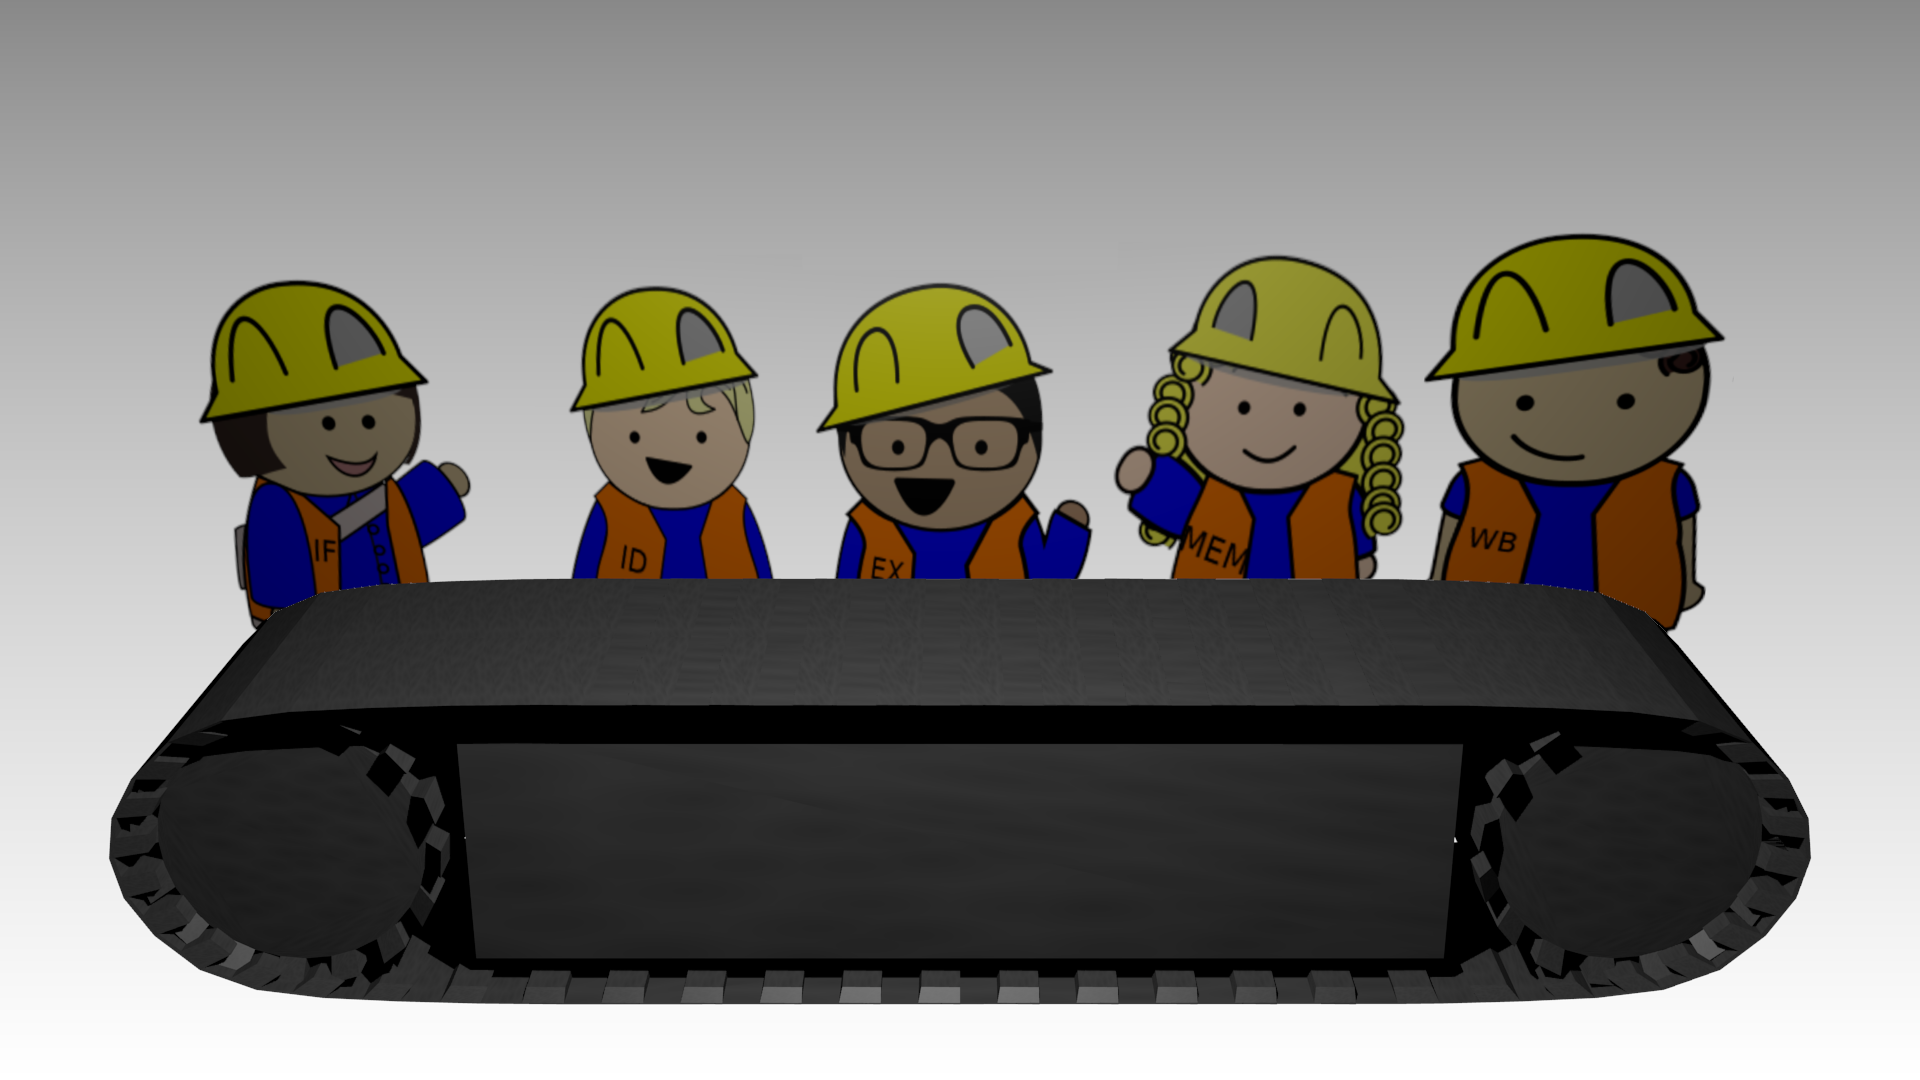
\includegraphics[width=1.0\textwidth]{final.png}}
	%FETCH
	\put(50,-12){\tiny\color{white}}
	
	%DECODE
	\put(90,-12){\tiny\color{white}}
	\put(90,-17){\tiny\color{white}}
	
	%EXECUTE
	\put(135,-12){\tiny\color{white}}
	\put(135,-17){\tiny\color{white}}
	\put(135,-22){\tiny\color{white}}
	
	%MEMORY
	\put(185,-12){\tiny\color{white}}
	\put(185,-17){\tiny\color{white}}
	\put(185,-22){\tiny\color{white}}
	
	%WRITEBACK
	\put(225,-12){\tiny\color{white}5:add t0, t0, 1}
	\put(225,-17){\tiny\color{white}5:t0 = 1 + 1}
	\put(225,-22){\tiny\color{white}5:t0 = 2}
	
	%REGISTERS
	\put(80,-37){\tiny\color{white}zero = 0}
	\put(80,-42){\tiny\color{white}ra = 0}
	\put(80,-47){\tiny\color{white}sp = 0}
	\put(80,-52){\tiny\color{white}pc = 36}
	\put(80,-57){\tiny\color{white}t0 = 2}
	\put(80,-62){\tiny\color{white}t1 = 0}
	
	\put(110,-37){\tiny\color{white}t2 = 0}
	\put(110,-42){\tiny\color{white}t3 = 0}
	\put(110,-47){\tiny\color{white}t4 = 0}
	\put(110,-52){\tiny\color{white}t5 = 0}
	\put(110,-57){\tiny\color{white}t6 = 0}
	\put(110,-62){\tiny\color{white}a0 = 0}
	
	\put(140,-37){\tiny\color{white}a1 = 0}
	\put(140,-42){\tiny\color{white}a2 = 0}
	\put(140,-47){\tiny\color{white}a3 = 0}
	\put(140,-52){\tiny\color{white}a4 = 0}
	\put(140,-57){\tiny\color{white}a5 = 0}
	\put(140,-62){\tiny\color{white}a6 = 0}
	
	\put(170,-37){\tiny\color{white}a7 = 0}
	\put(170,-42){\tiny\color{white}s1 = 0}
	\put(170,-47){\tiny\color{white}s2 = 0}
	\put(170,-52){\tiny\color{white}s3 = 0}
	\put(170,-57){\tiny\color{white}s4 = 0}
	\put(170,-62){\tiny\color{white}s5 = 0}
	
	\put(200,-37){\tiny\color{white}s6 = 0}
	\put(200,-42){\tiny\color{white}s7 = 0}
	\put(200,-47){\tiny\color{white}s8 = 0}
	\put(200,-52){\tiny\color{white}s9 = 0}
	\put(200,-57){\tiny\color{white}s10 = 0}
	\put(200,-62){\tiny\color{white}s11 = 0}
	
	\end{picture}
\end{frame}

\begin{frame}
	\frametitle{Pipeline Konflikt: Takt 10}
	\begin{picture}(0,0)
	\put(0,-85){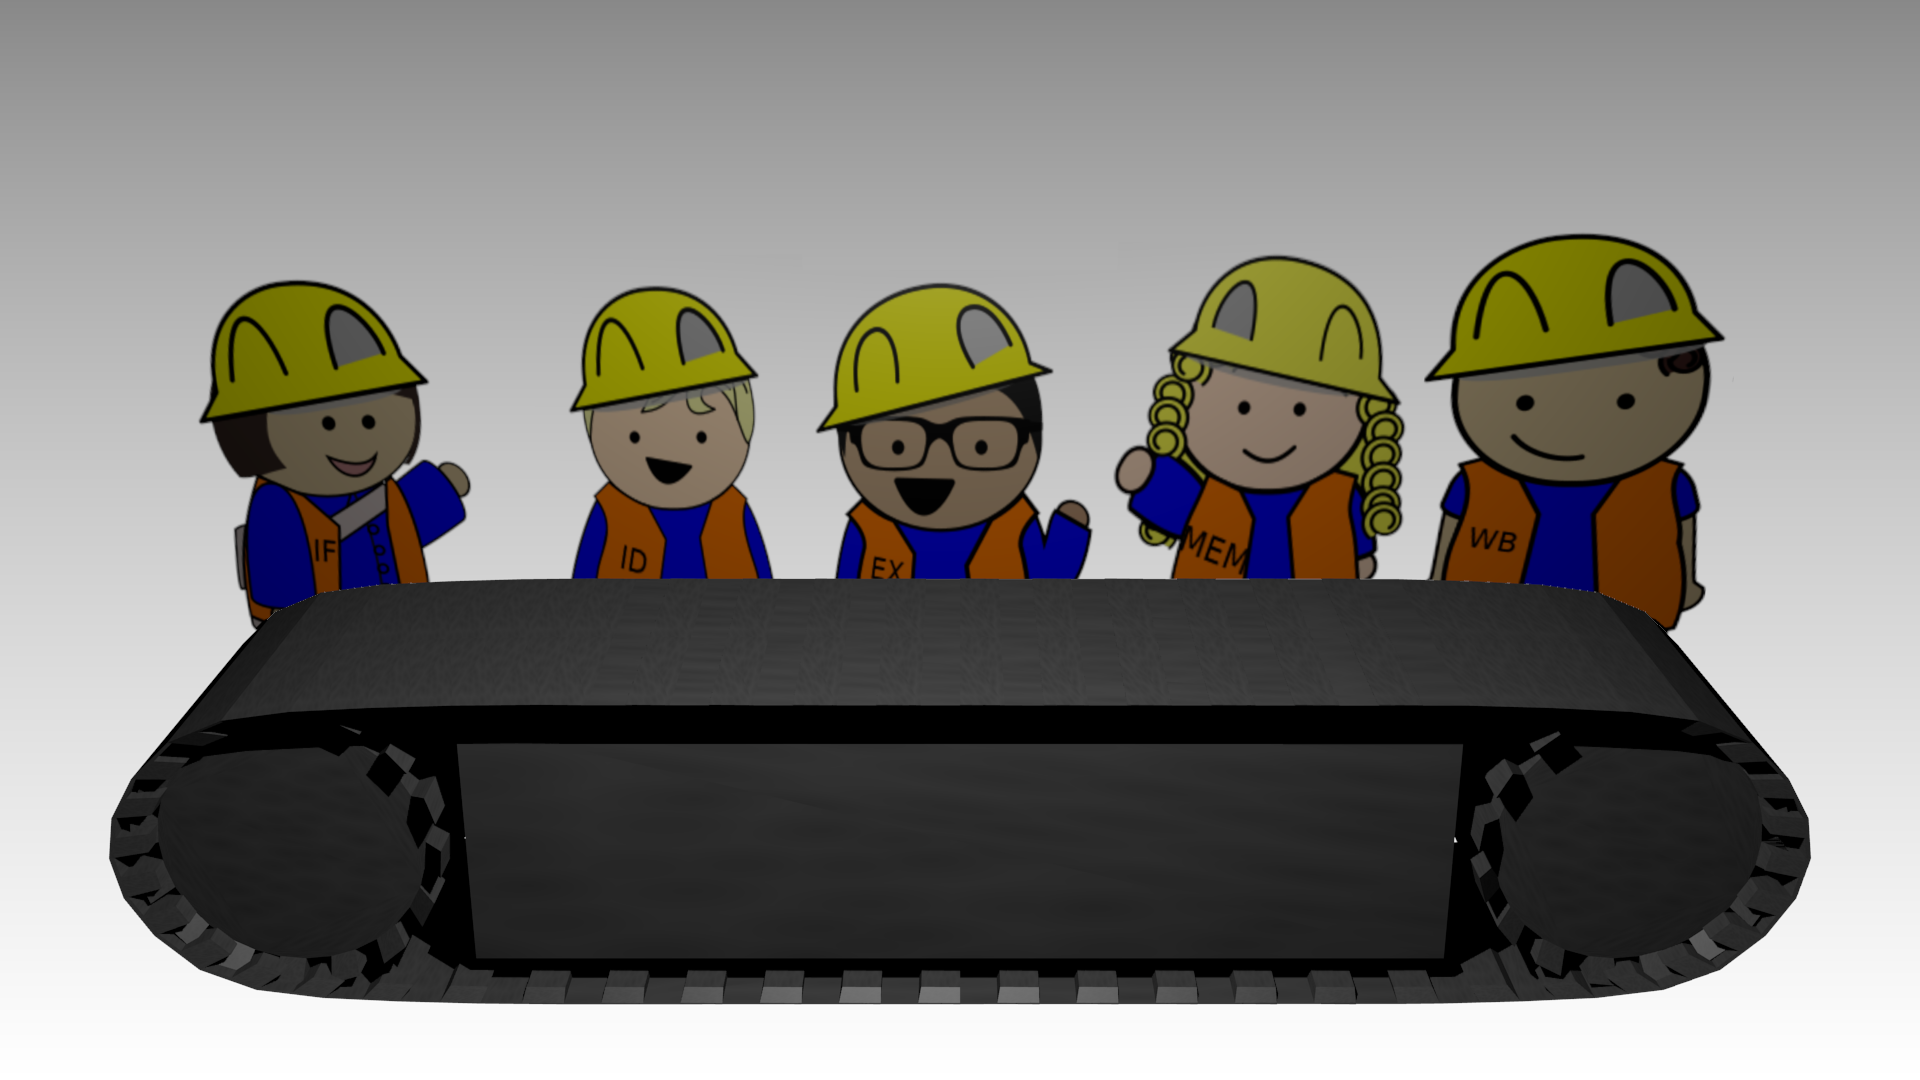
\includegraphics[width=1.0\textwidth]{final.png}}
	%FETCH
	\put(50,-12){\tiny\color{white}}
	
	%DECODE
	\put(90,-12){\tiny\color{white}}
	\put(90,-17){\tiny\color{white}}
	
	%EXECUTE
	\put(135,-12){\tiny\color{white}}
	\put(135,-17){\tiny\color{white}}
	\put(135,-22){\tiny\color{white}}
	
	%MEMORY
	\put(185,-12){\tiny\color{white}}
	\put(185,-17){\tiny\color{white}}
	\put(185,-22){\tiny\color{white}}
	
	%WRITEBACK
	\put(225,-12){\tiny\color{white}}
	\put(225,-17){\tiny\color{white}}
	\put(225,-22){\tiny\color{white}}
	
	%REGISTERS
	\put(80,-37){\tiny\color{white}zero = 0}
	\put(80,-42){\tiny\color{white}ra = 0}
	\put(80,-47){\tiny\color{white}sp = 0}
	\put(80,-52){\tiny\color{white}pc = 40}
	\put(80,-57){\tiny\color{white}t0 = 2}
	\put(80,-62){\tiny\color{white}t1 = 0}
	
	\put(110,-37){\tiny\color{white}t2 = 0}
	\put(110,-42){\tiny\color{white}t3 = 0}
	\put(110,-47){\tiny\color{white}t4 = 0}
	\put(110,-52){\tiny\color{white}t5 = 0}
	\put(110,-57){\tiny\color{white}t6 = 0}
	\put(110,-62){\tiny\color{white}a0 = 0}
	
	\put(140,-37){\tiny\color{white}a1 = 0}
	\put(140,-42){\tiny\color{white}a2 = 0}
	\put(140,-47){\tiny\color{white}a3 = 0}
	\put(140,-52){\tiny\color{white}a4 = 0}
	\put(140,-57){\tiny\color{white}a5 = 0}
	\put(140,-62){\tiny\color{white}a6 = 0}
	
	\put(170,-37){\tiny\color{white}a7 = 0}
	\put(170,-42){\tiny\color{white}s1 = 0}
	\put(170,-47){\tiny\color{white}s2 = 0}
	\put(170,-52){\tiny\color{white}s3 = 0}
	\put(170,-57){\tiny\color{white}s4 = 0}
	\put(170,-62){\tiny\color{white}s5 = 0}
	
	\put(200,-37){\tiny\color{white}s6 = 0}
	\put(200,-42){\tiny\color{white}s7 = 0}
	\put(200,-47){\tiny\color{white}s8 = 0}
	\put(200,-52){\tiny\color{white}s9 = 0}
	\put(200,-57){\tiny\color{white}s10 = 0}
	\put(200,-62){\tiny\color{white}s11 = 0}
	
	\end{picture}
\end{frame}

\begin{frame}
	\frametitle{Pipeline Konfliktlösung: Takt 0}
	\begin{picture}(0,0)
	\put(0,-85){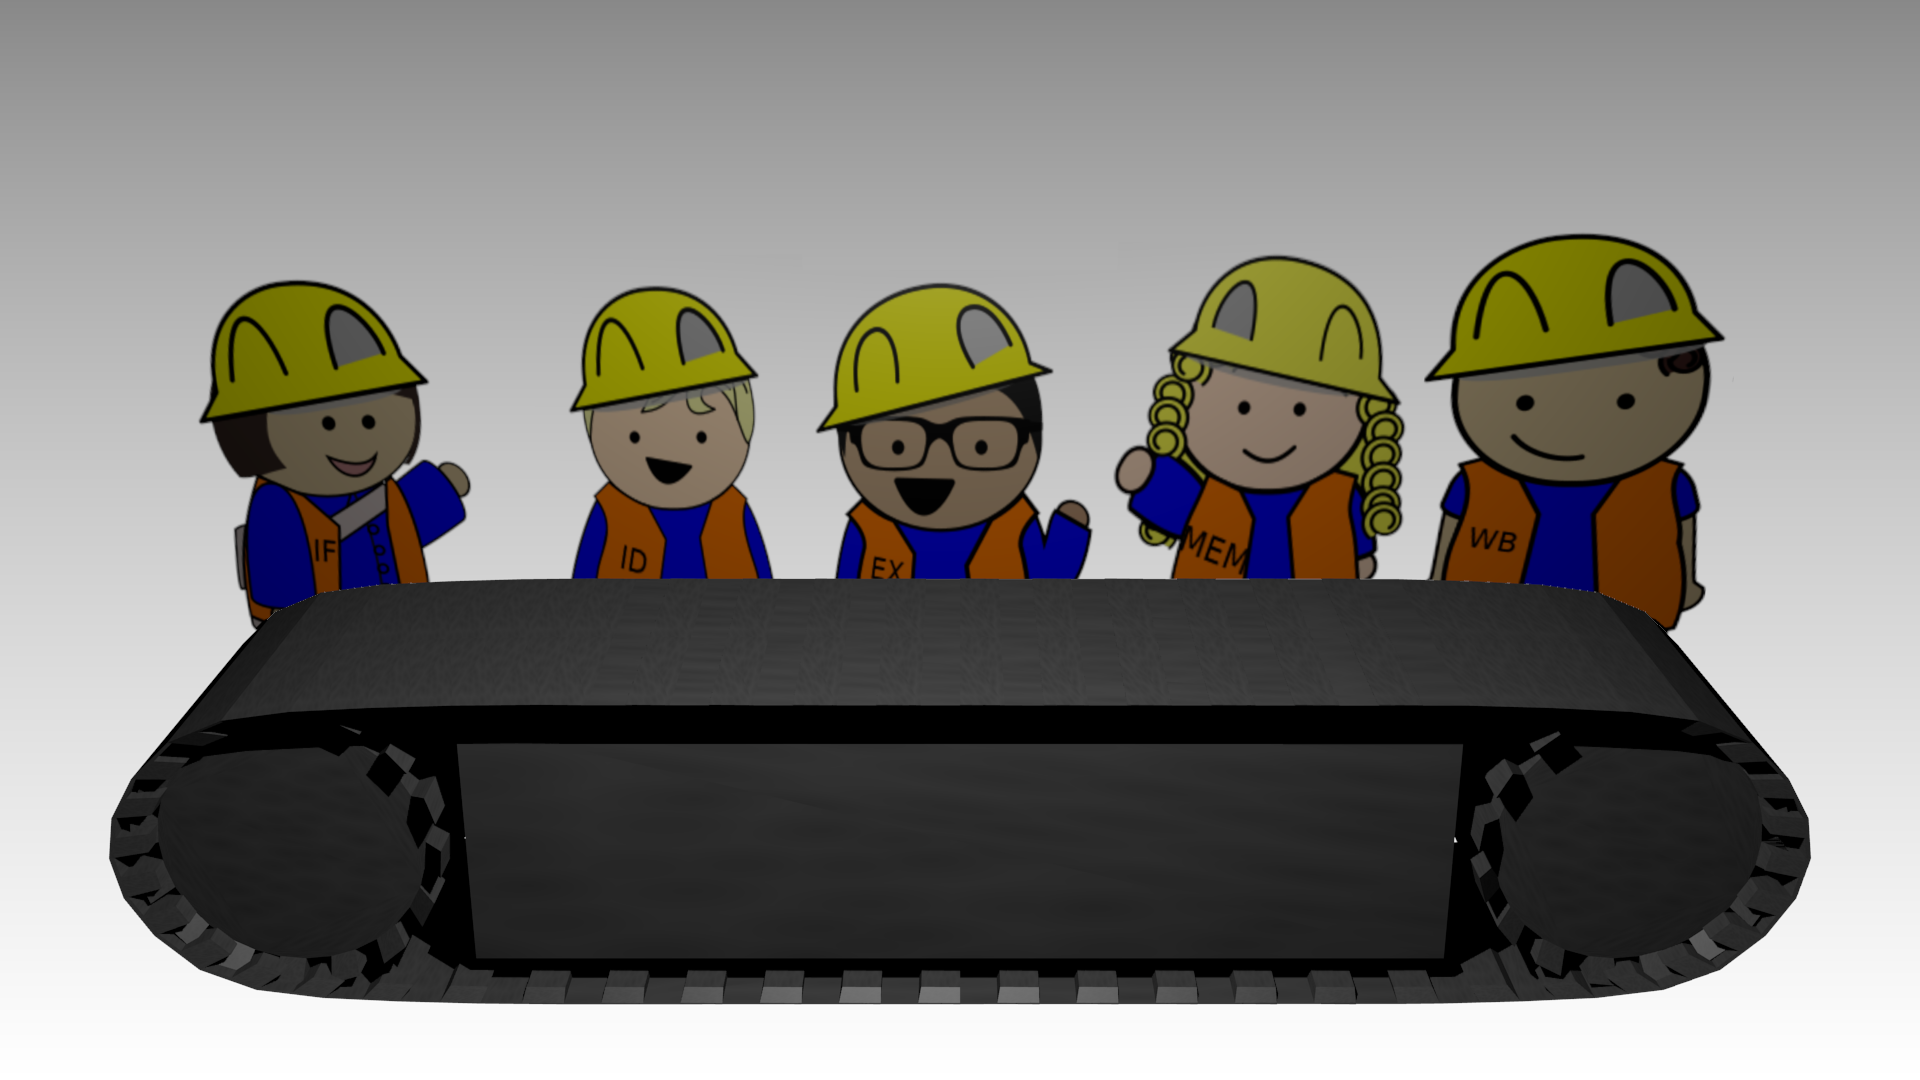
\includegraphics[width=1.0\textwidth]{final.png}}
	%FETCH
	\put(50,-12){\tiny\color{white}}
	
	%DECODE
	\put(90,-12){\tiny\color{white}}
	\put(90,-17){\tiny\color{white}}
	
	%EXECUTE
	\put(135,-12){\tiny\color{white}}
	\put(135,-17){\tiny\color{white}}
	\put(135,-22){\tiny\color{white}}
	
	%MEMORY
	\put(185,-12){\tiny\color{white}}
	\put(185,-17){\tiny\color{white}}
	\put(185,-22){\tiny\color{white}}
	
	%WRITEBACK
	\put(225,-12){\tiny\color{white}}
	\put(225,-17){\tiny\color{white}}
	\put(225,-22){\tiny\color{white}}
	
	%REGISTERS
	\put(80,-37){\tiny\color{white}zero = 0}
	\put(80,-42){\tiny\color{white}ra = 0}
	\put(80,-47){\tiny\color{white}sp = 0}
	\put(80,-52){\tiny\color{white}pc = 0}
	\put(80,-57){\tiny\color{white}t0 = 0}
	\put(80,-62){\tiny\color{white}t1 = 0}
	
	\put(110,-37){\tiny\color{white}t2 = 0}
	\put(110,-42){\tiny\color{white}t3 = 0}
	\put(110,-47){\tiny\color{white}t4 = 0}
	\put(110,-52){\tiny\color{white}t5 = 0}
	\put(110,-57){\tiny\color{white}t6 = 0}
	\put(110,-62){\tiny\color{white}a0 = 0}
	
	\put(140,-37){\tiny\color{white}a1 = 0}
	\put(140,-42){\tiny\color{white}a2 = 0}
	\put(140,-47){\tiny\color{white}a3 = 0}
	\put(140,-52){\tiny\color{white}a4 = 0}
	\put(140,-57){\tiny\color{white}a5 = 0}
	\put(140,-62){\tiny\color{white}a6 = 0}
	
	\put(170,-37){\tiny\color{white}a7 = 0}
	\put(170,-42){\tiny\color{white}s1 = 0}
	\put(170,-47){\tiny\color{white}s2 = 0}
	\put(170,-52){\tiny\color{white}s3 = 0}
	\put(170,-57){\tiny\color{white}s4 = 0}
	\put(170,-62){\tiny\color{white}s5 = 0}
	
	\put(200,-37){\tiny\color{white}s6 = 0}
	\put(200,-42){\tiny\color{white}s7 = 0}
	\put(200,-47){\tiny\color{white}s8 = 0}
	\put(200,-52){\tiny\color{white}s9 = 0}
	\put(200,-57){\tiny\color{white}s10 = 0}
	\put(200,-62){\tiny\color{white}s11 = 0}
	
	\end{picture}
\end{frame}


\begin{frame}
	\frametitle{Pipeline Konfliktlösung: Takt 1}
	\begin{picture}(0,0)
	\put(0,-85){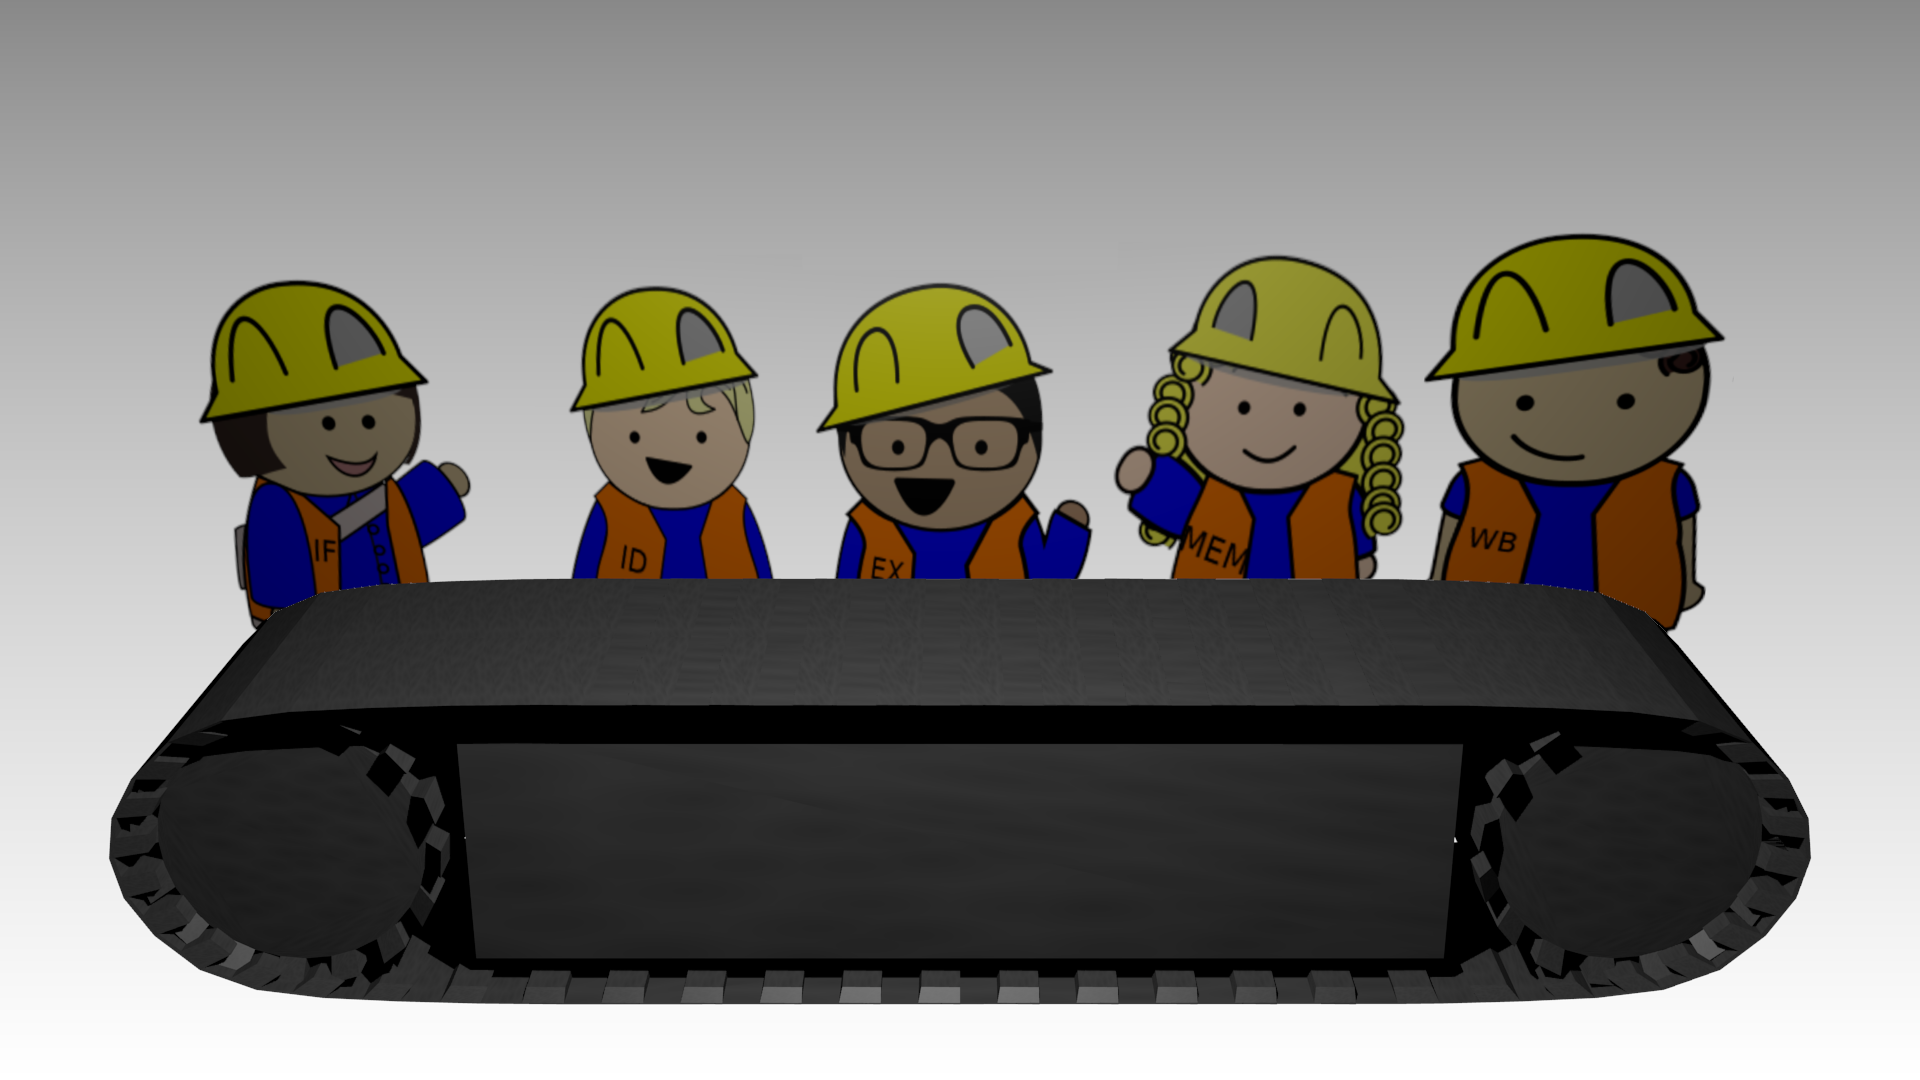
\includegraphics[width=1.0\textwidth]{final.png}}
	%FETCH
	\put(50,-12){\tiny\color{white}1:add t0, t0, 1}
	
	%DECODE
	\put(90,-12){\tiny\color{white}}
	\put(90,-17){\tiny\color{white}}
	
	%EXECUTE
	\put(135,-12){\tiny\color{white}}
	\put(135,-17){\tiny\color{white}}
	\put(135,-22){\tiny\color{white}}
	
	%MEMORY
	\put(185,-12){\tiny\color{white}}
	\put(185,-17){\tiny\color{white}}
	\put(185,-22){\tiny\color{white}}
	
	%WRITEBACK
	\put(225,-12){\tiny\color{white}}
	\put(225,-17){\tiny\color{white}}
	\put(225,-22){\tiny\color{white}}
	
	%REGISTERS
	\put(80,-37){\tiny\color{white}zero = 0}
	\put(80,-42){\tiny\color{white}ra = 0}
	\put(80,-47){\tiny\color{white}sp = 0}
	\put(80,-52){\tiny\color{white}pc = 4}
	\put(80,-57){\tiny\color{white}t0 = 0}
	\put(80,-62){\tiny\color{white}t1 = 0}
	
	\put(110,-37){\tiny\color{white}t2 = 0}
	\put(110,-42){\tiny\color{white}t3 = 0}
	\put(110,-47){\tiny\color{white}t4 = 0}
	\put(110,-52){\tiny\color{white}t5 = 0}
	\put(110,-57){\tiny\color{white}t6 = 0}
	\put(110,-62){\tiny\color{white}a0 = 0}
	
	\put(140,-37){\tiny\color{white}a1 = 0}
	\put(140,-42){\tiny\color{white}a2 = 0}
	\put(140,-47){\tiny\color{white}a3 = 0}
	\put(140,-52){\tiny\color{white}a4 = 0}
	\put(140,-57){\tiny\color{white}a5 = 0}
	\put(140,-62){\tiny\color{white}a6 = 0}
	
	\put(170,-37){\tiny\color{white}a7 = 0}
	\put(170,-42){\tiny\color{white}s1 = 0}
	\put(170,-47){\tiny\color{white}s2 = 0}
	\put(170,-52){\tiny\color{white}s3 = 0}
	\put(170,-57){\tiny\color{white}s4 = 0}
	\put(170,-62){\tiny\color{white}s5 = 0}
	
	\put(200,-37){\tiny\color{white}s6 = 0}
	\put(200,-42){\tiny\color{white}s7 = 0}
	\put(200,-47){\tiny\color{white}s8 = 0}
	\put(200,-52){\tiny\color{white}s9 = 0}
	\put(200,-57){\tiny\color{white}s10 = 0}
	\put(200,-62){\tiny\color{white}s11 = 0}
	
	\end{picture}
\end{frame}

\begin{frame}
	\frametitle{Pipeline Konfliktlösung: Takt 2}
	\begin{picture}(0,0)
	\put(0,-85){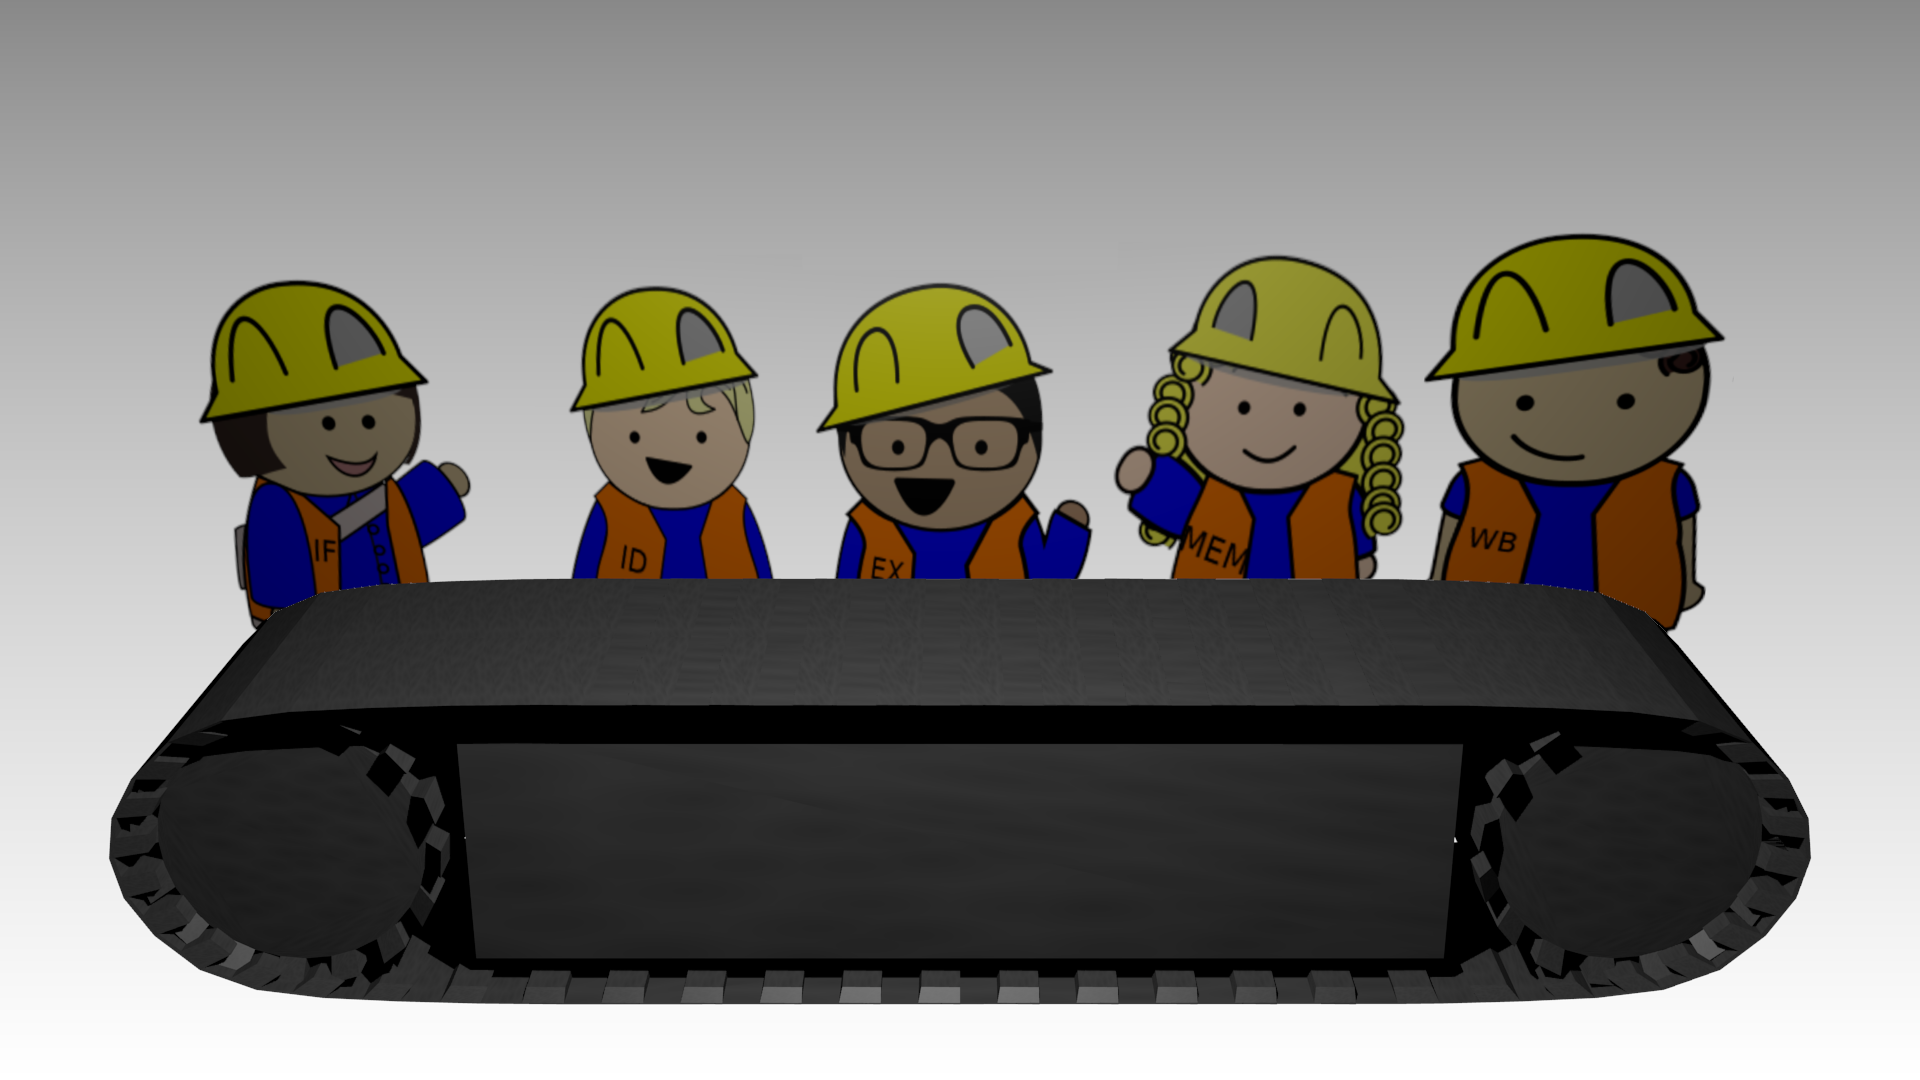
\includegraphics[width=1.0\textwidth]{final.png}}
	%FETCH
	\put(50,-12){\tiny\color{white}2:nop}
	
	%DECODE
	\put(90,-12){\tiny\color{white}1:add t0, t0, 1}
	\put(90,-17){\tiny\color{white}1:t0 = 0 + 1}
	
	%EXECUTE
	\put(135,-12){\tiny\color{white}}
	\put(135,-17){\tiny\color{white}}
	\put(135,-22){\tiny\color{white}}
	
	%MEMORY
	\put(185,-12){\tiny\color{white}}
	\put(185,-17){\tiny\color{white}}
	\put(185,-22){\tiny\color{white}}
	
	%WRITEBACK
	\put(225,-12){\tiny\color{white}}
	\put(225,-17){\tiny\color{white}}
	\put(225,-22){\tiny\color{white}}
	
	%REGISTERS
	\put(80,-37){\tiny\color{white}zero = 0}
	\put(80,-42){\tiny\color{white}ra = 0}
	\put(80,-47){\tiny\color{white}sp = 0}
	\put(80,-52){\tiny\color{white}pc = 8}
	\put(80,-57){\tiny\color{white}t0 = 0}
	\put(80,-62){\tiny\color{white}t1 = 0}
	
	\put(110,-37){\tiny\color{white}t2 = 0}
	\put(110,-42){\tiny\color{white}t3 = 0}
	\put(110,-47){\tiny\color{white}t4 = 0}
	\put(110,-52){\tiny\color{white}t5 = 0}
	\put(110,-57){\tiny\color{white}t6 = 0}
	\put(110,-62){\tiny\color{white}a0 = 0}
	
	\put(140,-37){\tiny\color{white}a1 = 0}
	\put(140,-42){\tiny\color{white}a2 = 0}
	\put(140,-47){\tiny\color{white}a3 = 0}
	\put(140,-52){\tiny\color{white}a4 = 0}
	\put(140,-57){\tiny\color{white}a5 = 0}
	\put(140,-62){\tiny\color{white}a6 = 0}
	
	\put(170,-37){\tiny\color{white}a7 = 0}
	\put(170,-42){\tiny\color{white}s1 = 0}
	\put(170,-47){\tiny\color{white}s2 = 0}
	\put(170,-52){\tiny\color{white}s3 = 0}
	\put(170,-57){\tiny\color{white}s4 = 0}
	\put(170,-62){\tiny\color{white}s5 = 0}
	
	\put(200,-37){\tiny\color{white}s6 = 0}
	\put(200,-42){\tiny\color{white}s7 = 0}
	\put(200,-47){\tiny\color{white}s8 = 0}
	\put(200,-52){\tiny\color{white}s9 = 0}
	\put(200,-57){\tiny\color{white}s10 = 0}
	\put(200,-62){\tiny\color{white}s11 = 0}
	
	\end{picture}
\end{frame}

\begin{frame}
	\frametitle{Pipeline Konfliktlösung: Takt 3}
	\begin{picture}(0,0)
	\put(0,-85){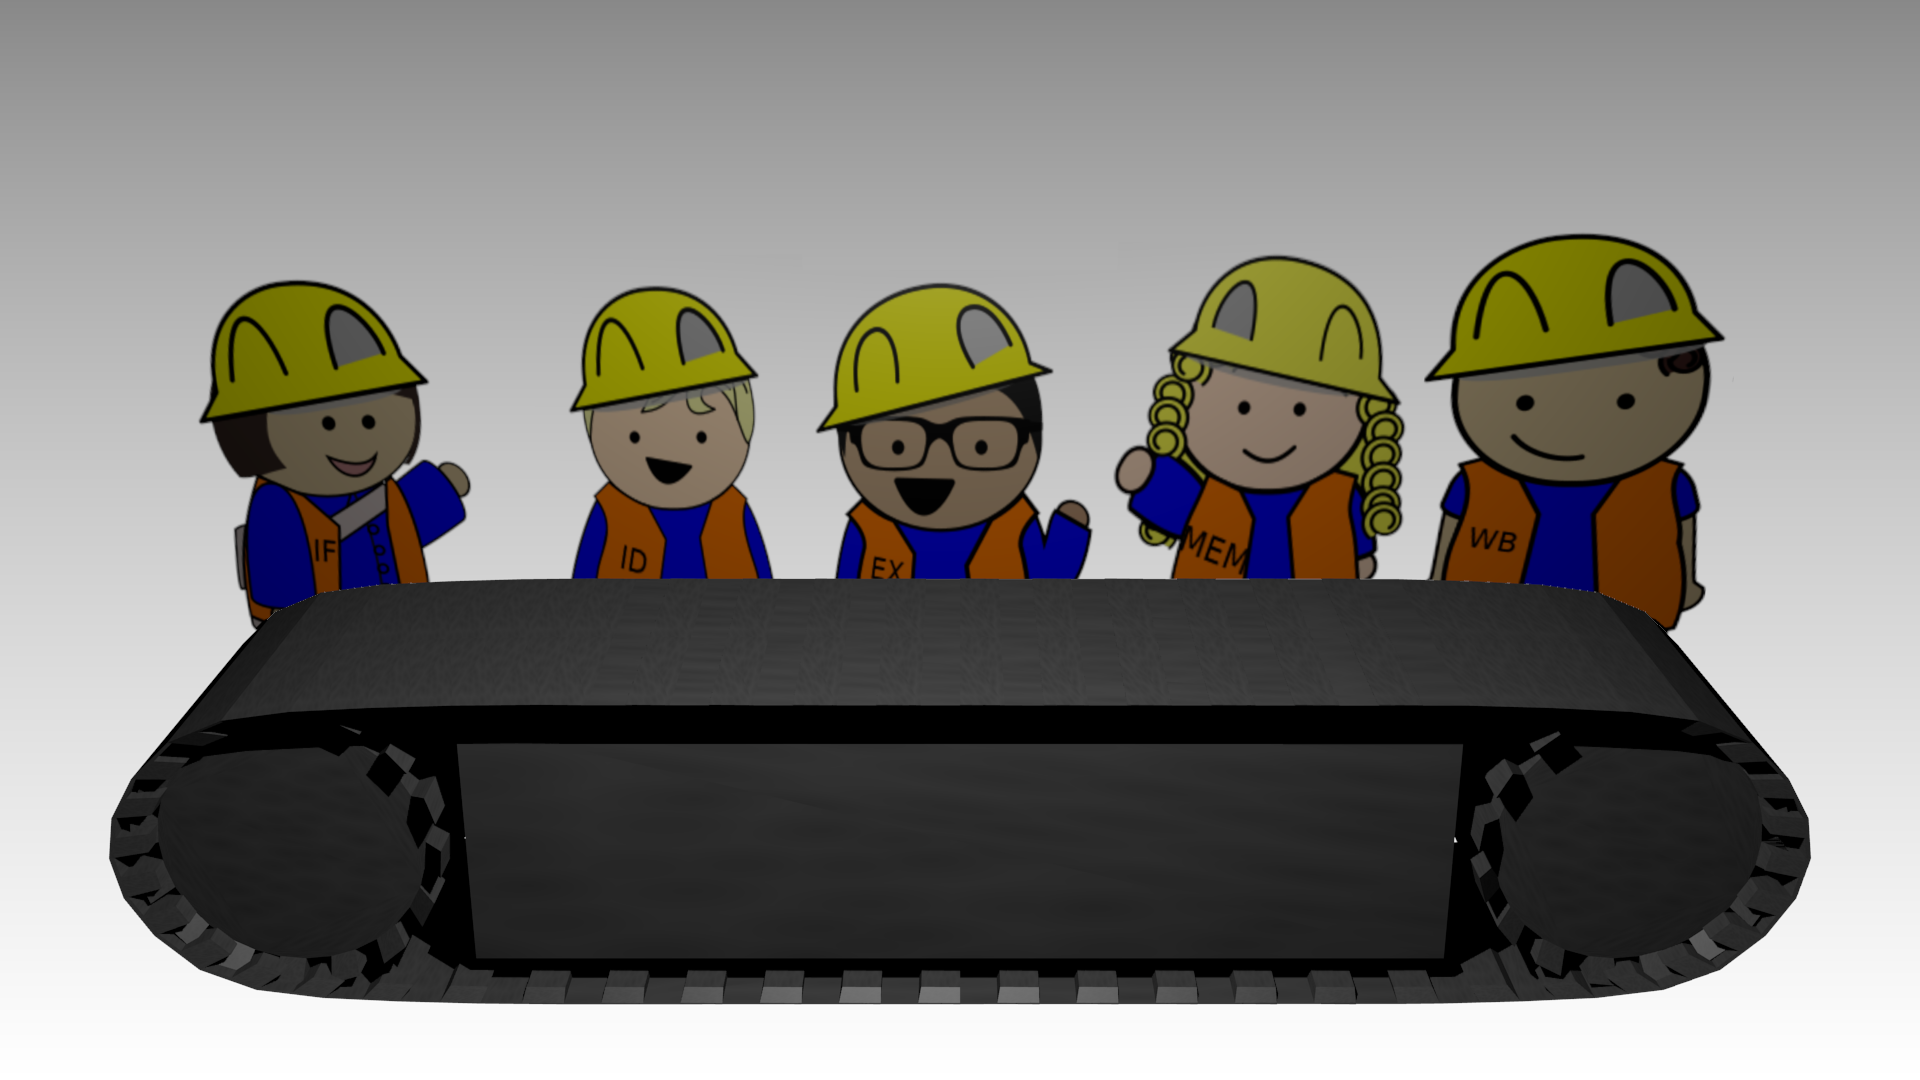
\includegraphics[width=1.0\textwidth]{final.png}}
	%FETCH
	\put(50,-12){\tiny\color{white}3:nop}
	
	%DECODE
	\put(90,-12){\tiny\color{white}2:nop}
	\put(90,-17){\tiny\color{white}}
	
	%EXECUTE
	\put(135,-12){\tiny\color{white}1:add t0, t0, 1}
	\put(135,-17){\tiny\color{white}1:t0 = 0 + 1}
	\put(135,-22){\tiny\color{white}1:t0 = 1}
	
	%MEMORY
	\put(185,-12){\tiny\color{white}}
	\put(185,-17){\tiny\color{white}}
	\put(185,-22){\tiny\color{white}}
	
	%WRITEBACK
	\put(225,-12){\tiny\color{white}}
	\put(225,-17){\tiny\color{white}}
	\put(225,-22){\tiny\color{white}}
	
	%REGISTERS
	\put(80,-37){\tiny\color{white}zero = 0}
	\put(80,-42){\tiny\color{white}ra = 0}
	\put(80,-47){\tiny\color{white}sp = 0}
	\put(80,-52){\tiny\color{white}pc = 12}
	\put(80,-57){\tiny\color{white}t0 = 0}
	\put(80,-62){\tiny\color{white}t1 = 0}
	
	\put(110,-37){\tiny\color{white}t2 = 0}
	\put(110,-42){\tiny\color{white}t3 = 0}
	\put(110,-47){\tiny\color{white}t4 = 0}
	\put(110,-52){\tiny\color{white}t5 = 0}
	\put(110,-57){\tiny\color{white}t6 = 0}
	\put(110,-62){\tiny\color{white}a0 = 0}
	
	\put(140,-37){\tiny\color{white}a1 = 0}
	\put(140,-42){\tiny\color{white}a2 = 0}
	\put(140,-47){\tiny\color{white}a3 = 0}
	\put(140,-52){\tiny\color{white}a4 = 0}
	\put(140,-57){\tiny\color{white}a5 = 0}
	\put(140,-62){\tiny\color{white}a6 = 0}
	
	\put(170,-37){\tiny\color{white}a7 = 0}
	\put(170,-42){\tiny\color{white}s1 = 0}
	\put(170,-47){\tiny\color{white}s2 = 0}
	\put(170,-52){\tiny\color{white}s3 = 0}
	\put(170,-57){\tiny\color{white}s4 = 0}
	\put(170,-62){\tiny\color{white}s5 = 0}
	
	\put(200,-37){\tiny\color{white}s6 = 0}
	\put(200,-42){\tiny\color{white}s7 = 0}
	\put(200,-47){\tiny\color{white}s8 = 0}
	\put(200,-52){\tiny\color{white}s9 = 0}
	\put(200,-57){\tiny\color{white}s10 = 0}
	\put(200,-62){\tiny\color{white}s11 = 0}
	
	\end{picture}
\end{frame}

\begin{frame}
	\frametitle{Pipeline Konfliktlösung: Takt 4}
	\begin{picture}(0,0)
	\put(0,-85){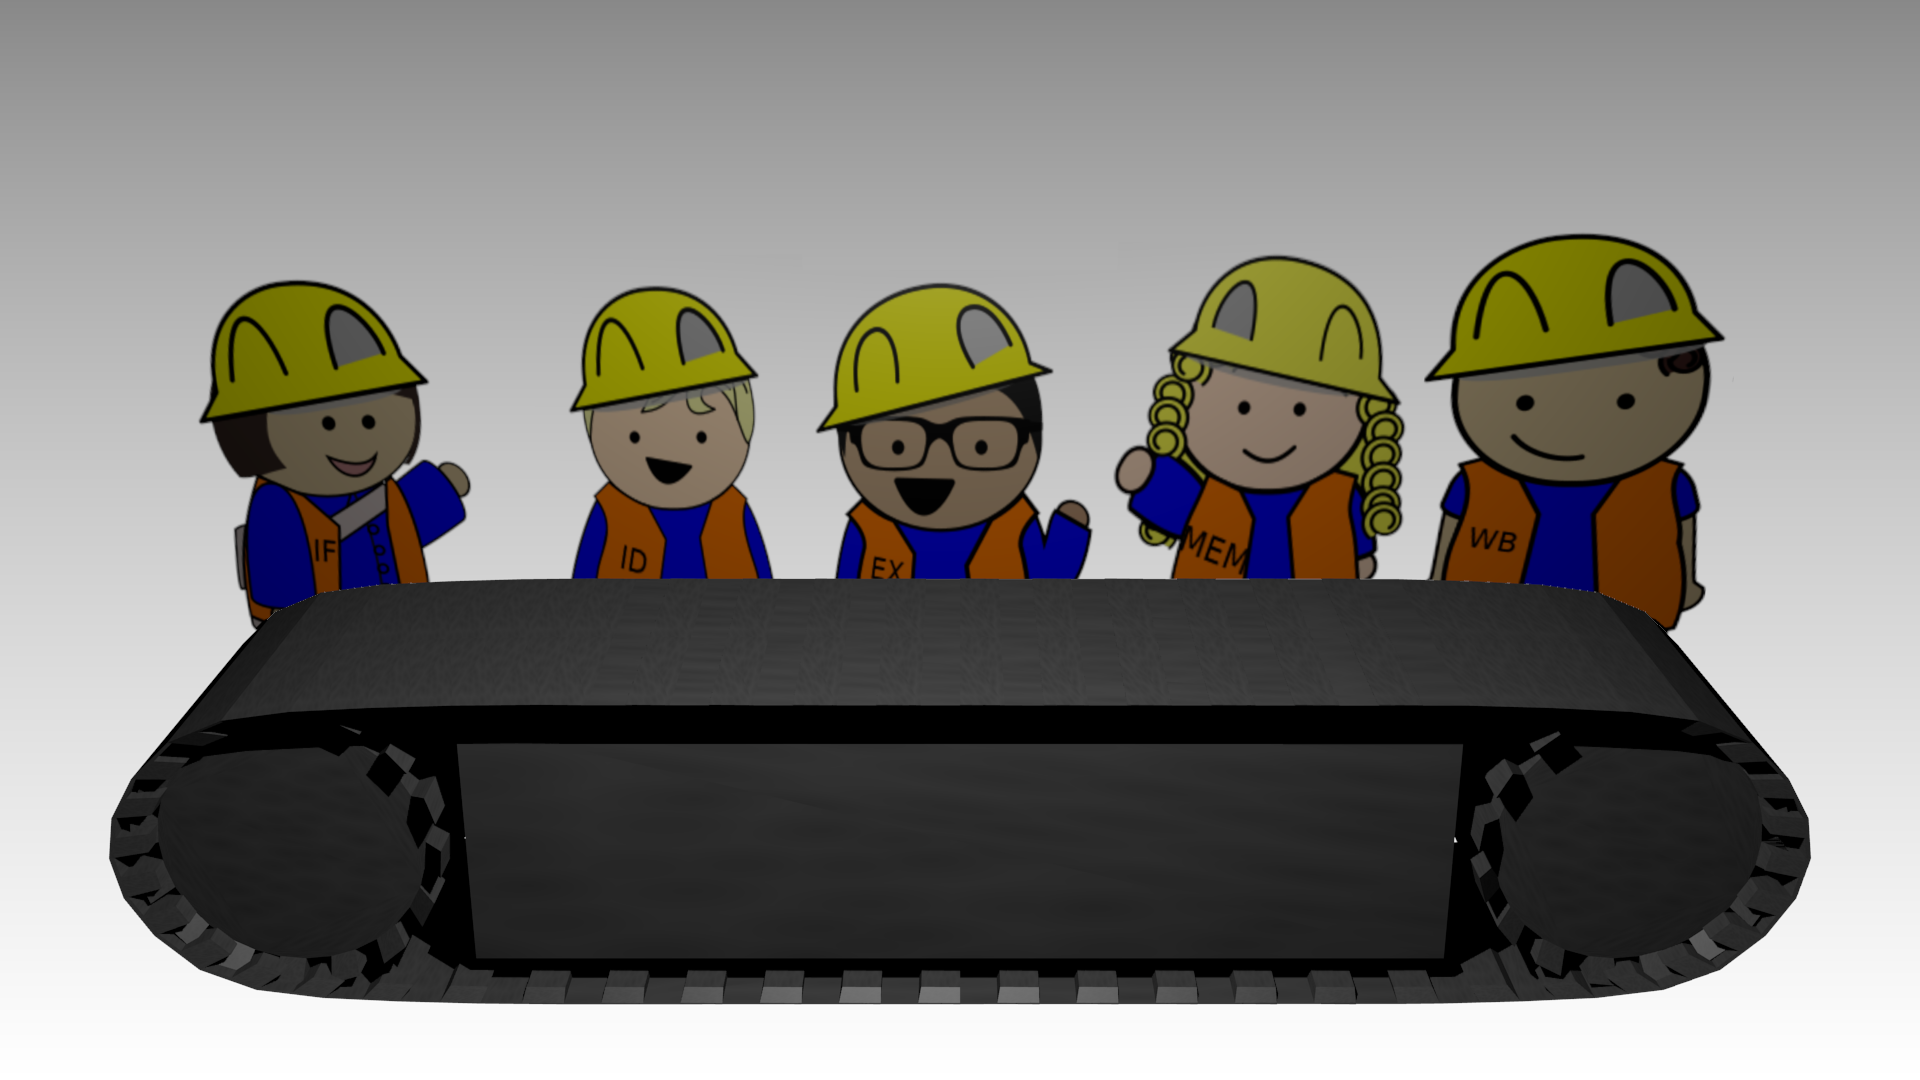
\includegraphics[width=1.0\textwidth]{final.png}}
	%FETCH
	\put(50,-12){\tiny\color{white}4:add t0, t0, 1}
	
	%DECODE
	\put(90,-12){\tiny\color{white}3:nop}
	\put(90,-17){\tiny\color{white}}
	
	%EXECUTE
	\put(135,-12){\tiny\color{white}2:nop}
	\put(135,-17){\tiny\color{white}}
	\put(135,-22){\tiny\color{white}}
	
	%MEMORY
	\put(185,-12){\tiny\color{white}1:add t0, t0, 1}
	\put(185,-17){\tiny\color{white}1:t0 = 0 + 1}
	\put(185,-22){\tiny\color{white}1:t0 = 1}
	
	%WRITEBACK
	\put(225,-12){\tiny\color{white}}
	\put(225,-17){\tiny\color{white}}
	\put(225,-22){\tiny\color{white}}
	
	%REGISTERS
	\put(80,-37){\tiny\color{white}zero = 0}
	\put(80,-42){\tiny\color{white}ra = 0}
	\put(80,-47){\tiny\color{white}sp = 0}
	\put(80,-52){\tiny\color{white}pc = 16}
	\put(80,-57){\tiny\color{white}t0 = 0}
	\put(80,-62){\tiny\color{white}t1 = 0}
	
	\put(110,-37){\tiny\color{white}t2 = 0}
	\put(110,-42){\tiny\color{white}t3 = 0}
	\put(110,-47){\tiny\color{white}t4 = 0}
	\put(110,-52){\tiny\color{white}t5 = 0}
	\put(110,-57){\tiny\color{white}t6 = 0}
	\put(110,-62){\tiny\color{white}a0 = 0}
	
	\put(140,-37){\tiny\color{white}a1 = 0}
	\put(140,-42){\tiny\color{white}a2 = 0}
	\put(140,-47){\tiny\color{white}a3 = 0}
	\put(140,-52){\tiny\color{white}a4 = 0}
	\put(140,-57){\tiny\color{white}a5 = 0}
	\put(140,-62){\tiny\color{white}a6 = 0}
	
	\put(170,-37){\tiny\color{white}a7 = 0}
	\put(170,-42){\tiny\color{white}s1 = 0}
	\put(170,-47){\tiny\color{white}s2 = 0}
	\put(170,-52){\tiny\color{white}s3 = 0}
	\put(170,-57){\tiny\color{white}s4 = 0}
	\put(170,-62){\tiny\color{white}s5 = 0}
	
	\put(200,-37){\tiny\color{white}s6 = 0}
	\put(200,-42){\tiny\color{white}s7 = 0}
	\put(200,-47){\tiny\color{white}s8 = 0}
	\put(200,-52){\tiny\color{white}s9 = 0}
	\put(200,-57){\tiny\color{white}s10 = 0}
	\put(200,-62){\tiny\color{white}s11 = 0}
	
	\end{picture}
\end{frame}

\begin{frame}
	\frametitle{Pipeline Konfliktlösung: Takt 5}
	\begin{picture}(0,0)
	\put(0,-85){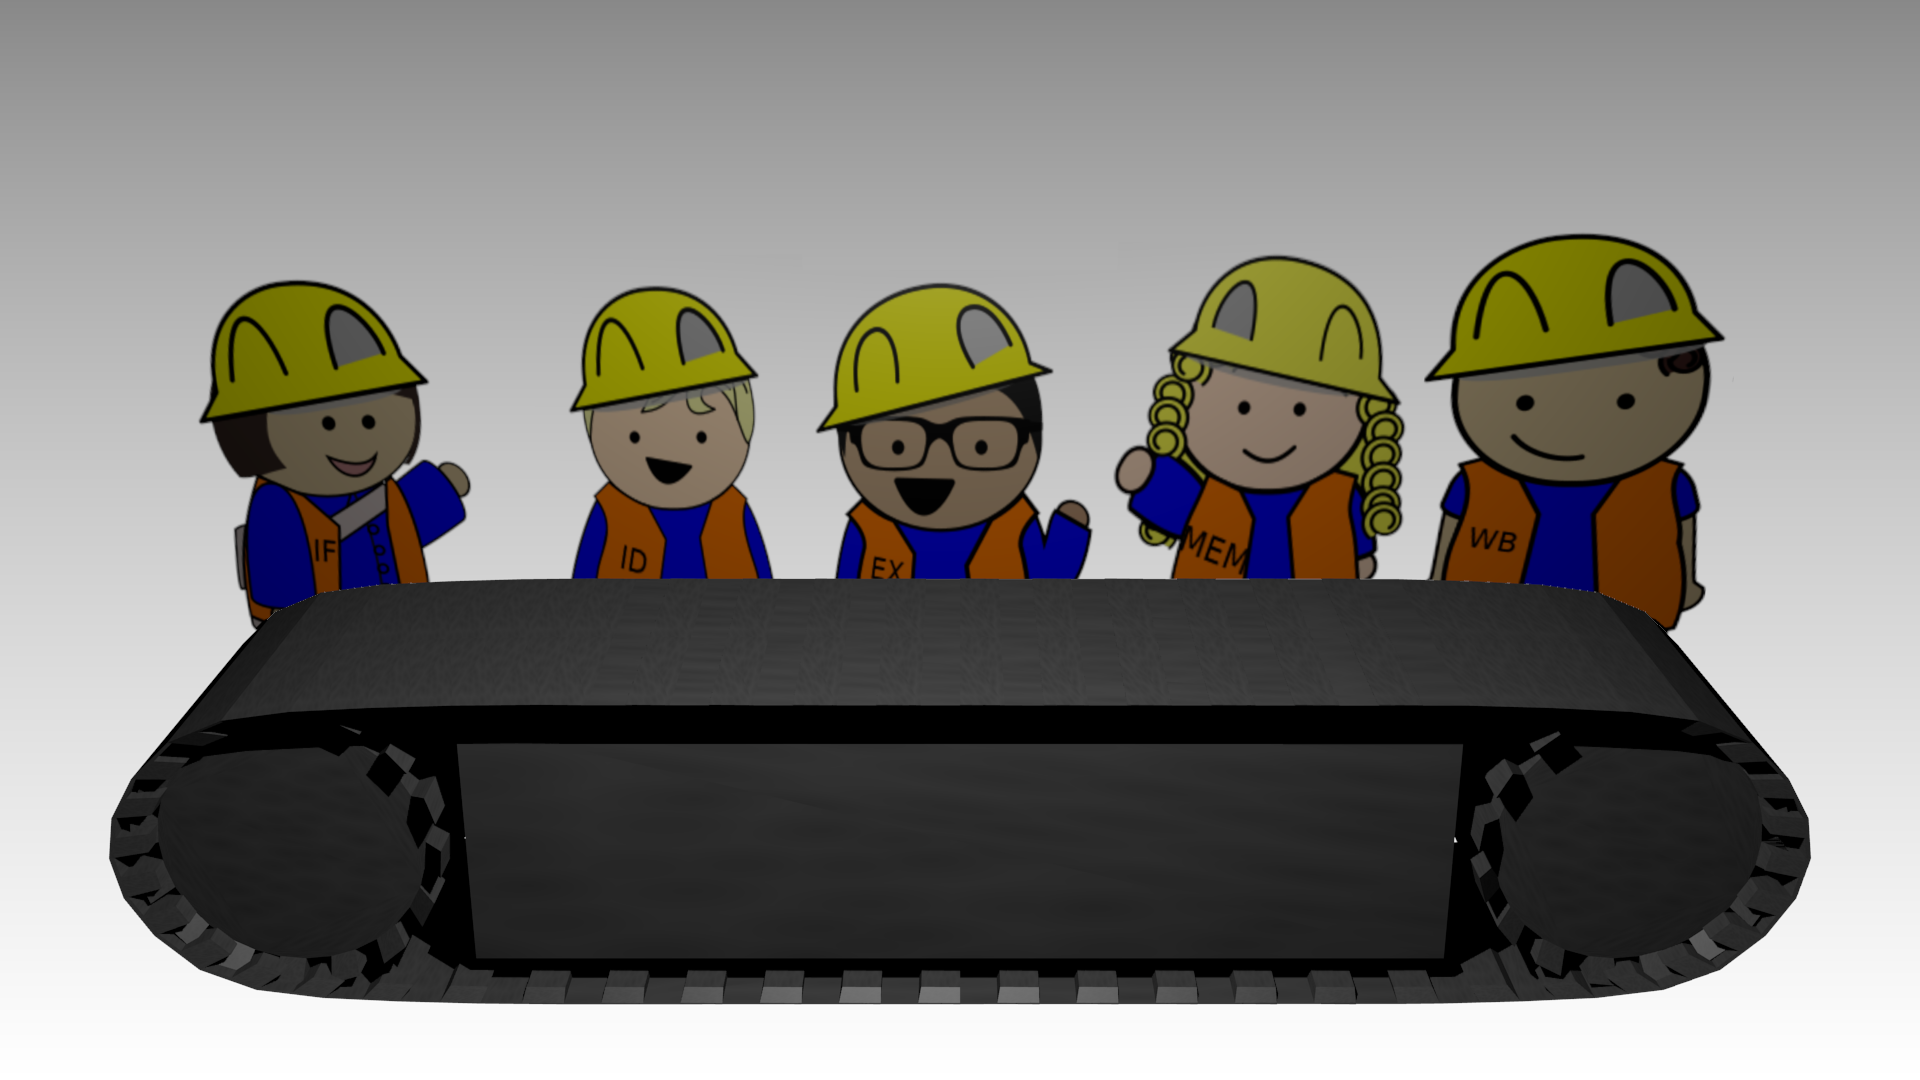
\includegraphics[width=1.0\textwidth]{final.png}}
	%FETCH
	\put(50,-12){\tiny\color{white}5:nop}
	
	%DECODE
	\put(90,-12){\tiny\color{white}4:add t0, t0, 1}
	\put(90,-17){\tiny\color{white}4:t0 = 1 + 1}
	
	%EXECUTE
	\put(135,-12){\tiny\color{white}3:nop}
	\put(135,-17){\tiny\color{white}}
	\put(135,-22){\tiny\color{white}}
	
	%MEMORY
	\put(185,-12){\tiny\color{white}2:nop}
	\put(185,-17){\tiny\color{white}}
	\put(185,-22){\tiny\color{white}}
	
	%WRITEBACK
	\put(225,-12){\tiny\color{white}1:add t0, t0, 1}
	\put(225,-17){\tiny\color{white}1:t0 = 0 + 1}
	\put(225,-22){\tiny\color{white}1:t0 = 1}
	
	%REGISTERS
	\put(80,-37){\tiny\color{white}zero = 0}
	\put(80,-42){\tiny\color{white}ra = 0}
	\put(80,-47){\tiny\color{white}sp = 0}
	\put(80,-52){\tiny\color{white}pc = 20}
	\put(80,-57){\tiny\color{white}t0 = 1}
	\put(80,-62){\tiny\color{white}t1 = 0}
	
	\put(110,-37){\tiny\color{white}t2 = 0}
	\put(110,-42){\tiny\color{white}t3 = 0}
	\put(110,-47){\tiny\color{white}t4 = 0}
	\put(110,-52){\tiny\color{white}t5 = 0}
	\put(110,-57){\tiny\color{white}t6 = 0}
	\put(110,-62){\tiny\color{white}a0 = 0}
	
	\put(140,-37){\tiny\color{white}a1 = 0}
	\put(140,-42){\tiny\color{white}a2 = 0}
	\put(140,-47){\tiny\color{white}a3 = 0}
	\put(140,-52){\tiny\color{white}a4 = 0}
	\put(140,-57){\tiny\color{white}a5 = 0}
	\put(140,-62){\tiny\color{white}a6 = 0}
	
	\put(170,-37){\tiny\color{white}a7 = 0}
	\put(170,-42){\tiny\color{white}s1 = 0}
	\put(170,-47){\tiny\color{white}s2 = 0}
	\put(170,-52){\tiny\color{white}s3 = 0}
	\put(170,-57){\tiny\color{white}s4 = 0}
	\put(170,-62){\tiny\color{white}s5 = 0}
	
	\put(200,-37){\tiny\color{white}s6 = 0}
	\put(200,-42){\tiny\color{white}s7 = 0}
	\put(200,-47){\tiny\color{white}s8 = 0}
	\put(200,-52){\tiny\color{white}s9 = 0}
	\put(200,-57){\tiny\color{white}s10 = 0}
	\put(200,-62){\tiny\color{white}s11 = 0}
	
	\end{picture}
\end{frame}

\begin{frame}
	\frametitle{Pipeline Konfliktlösung: Takt 6}
	\begin{picture}(0,0)
	\put(0,-85){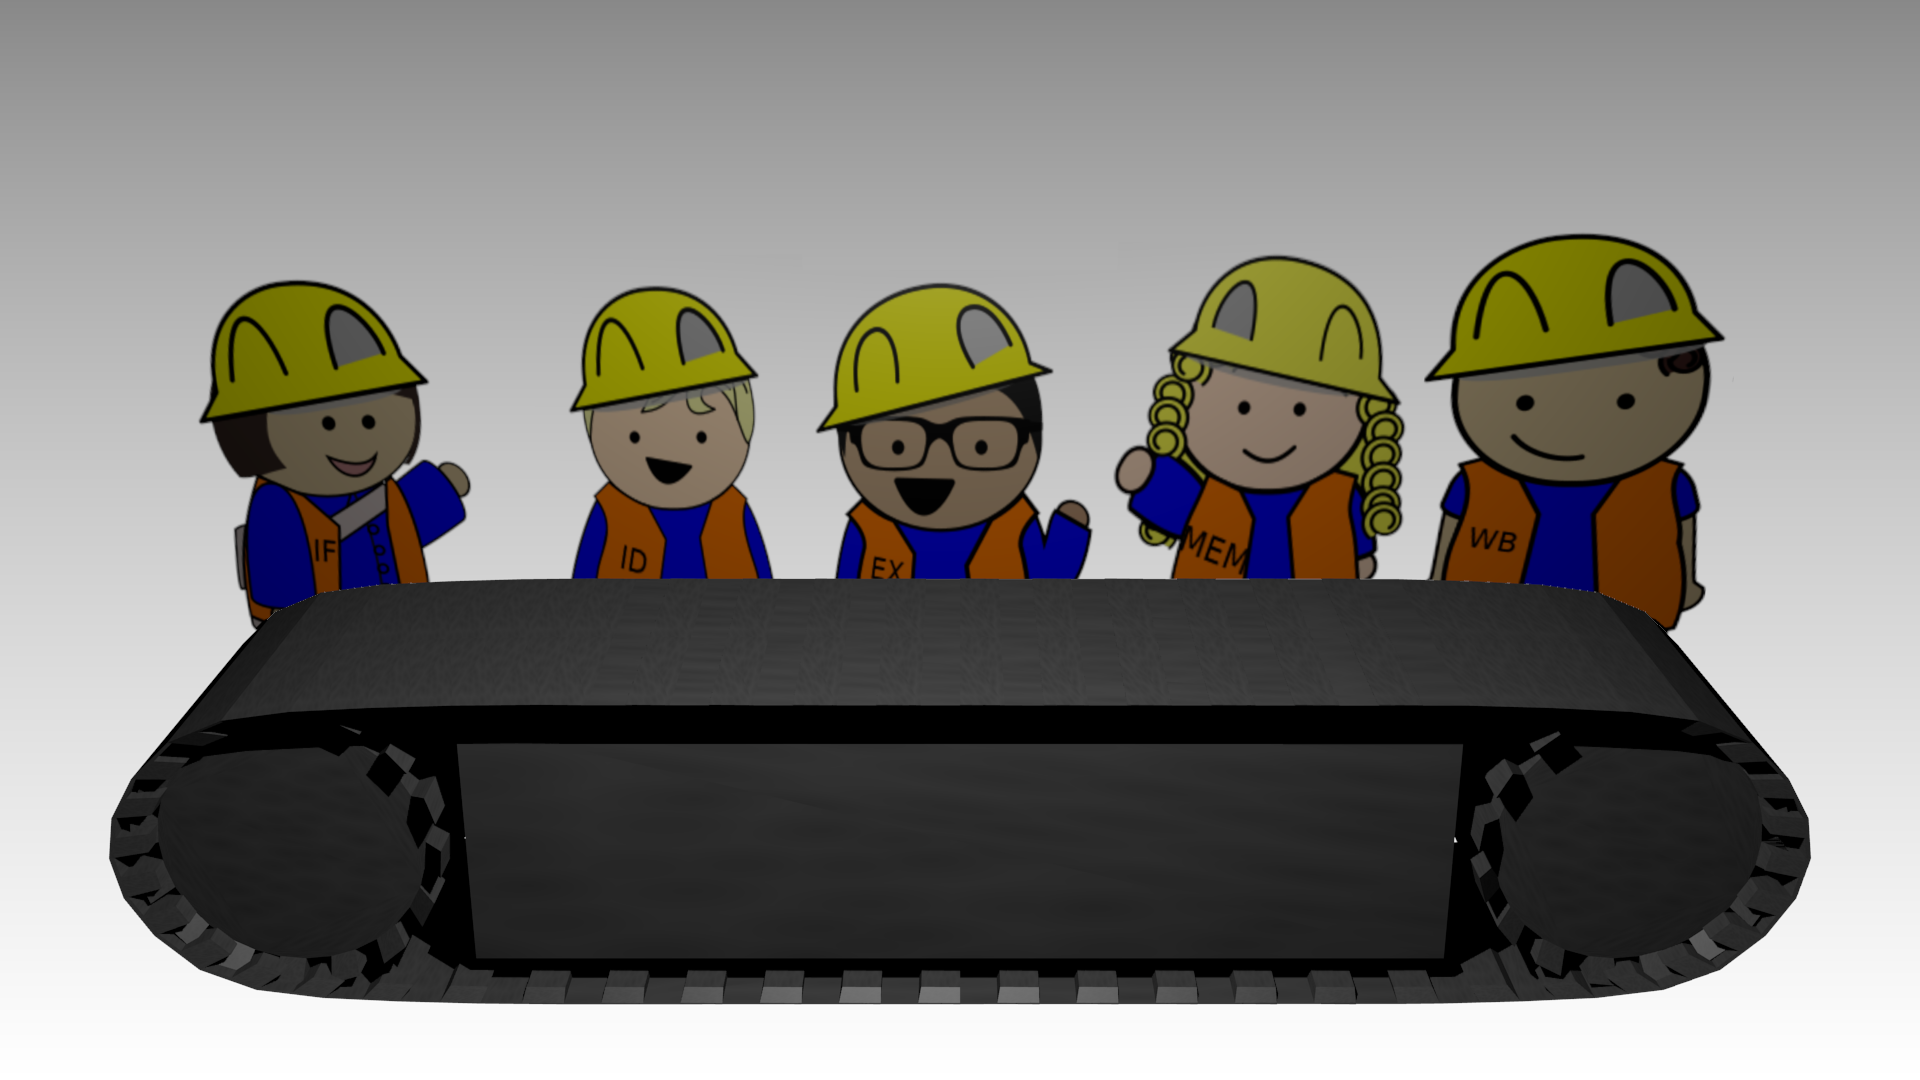
\includegraphics[width=1.0\textwidth]{final.png}}
	%FETCH
	\put(50,-12){\tiny\color{white}6:nop}
	
	%DECODE
	\put(90,-12){\tiny\color{white}5:nop}
	\put(90,-17){\tiny\color{white}}
	
	%EXECUTE
	\put(135,-12){\tiny\color{white}4:add t0, t0, 1}
	\put(135,-17){\tiny\color{white}4:t0 = 1 + 1}
	\put(135,-22){\tiny\color{white}4:t0 = 2}
	
	%MEMORY
	\put(185,-12){\tiny\color{white}3:nop}
	\put(185,-17){\tiny\color{white}}
	\put(185,-22){\tiny\color{white}}
	
	%WRITEBACK
	\put(225,-12){\tiny\color{white}2:nop}
	\put(225,-17){\tiny\color{white}}
	\put(225,-22){\tiny\color{white}}
	
	%REGISTERS
	\put(80,-37){\tiny\color{white}zero = 0}
	\put(80,-42){\tiny\color{white}ra = 0}
	\put(80,-47){\tiny\color{white}sp = 0}
	\put(80,-52){\tiny\color{white}pc = 24}
	\put(80,-57){\tiny\color{white}t0 = 1}
	\put(80,-62){\tiny\color{white}t1 = 0}
	
	\put(110,-37){\tiny\color{white}t2 = 0}
	\put(110,-42){\tiny\color{white}t3 = 0}
	\put(110,-47){\tiny\color{white}t4 = 0}
	\put(110,-52){\tiny\color{white}t5 = 0}
	\put(110,-57){\tiny\color{white}t6 = 0}
	\put(110,-62){\tiny\color{white}a0 = 0}
	
	\put(140,-37){\tiny\color{white}a1 = 0}
	\put(140,-42){\tiny\color{white}a2 = 0}
	\put(140,-47){\tiny\color{white}a3 = 0}
	\put(140,-52){\tiny\color{white}a4 = 0}
	\put(140,-57){\tiny\color{white}a5 = 0}
	\put(140,-62){\tiny\color{white}a6 = 0}
	
	\put(170,-37){\tiny\color{white}a7 = 0}
	\put(170,-42){\tiny\color{white}s1 = 0}
	\put(170,-47){\tiny\color{white}s2 = 0}
	\put(170,-52){\tiny\color{white}s3 = 0}
	\put(170,-57){\tiny\color{white}s4 = 0}
	\put(170,-62){\tiny\color{white}s5 = 0}
	
	\put(200,-37){\tiny\color{white}s6 = 0}
	\put(200,-42){\tiny\color{white}s7 = 0}
	\put(200,-47){\tiny\color{white}s8 = 0}
	\put(200,-52){\tiny\color{white}s9 = 0}
	\put(200,-57){\tiny\color{white}s10 = 0}
	\put(200,-62){\tiny\color{white}s11 = 0}
	
	\end{picture}
\end{frame}

\begin{frame}
	\frametitle{Pipeline Konfliktlösung: Takt 7}
	\begin{picture}(0,0)
	\put(0,-85){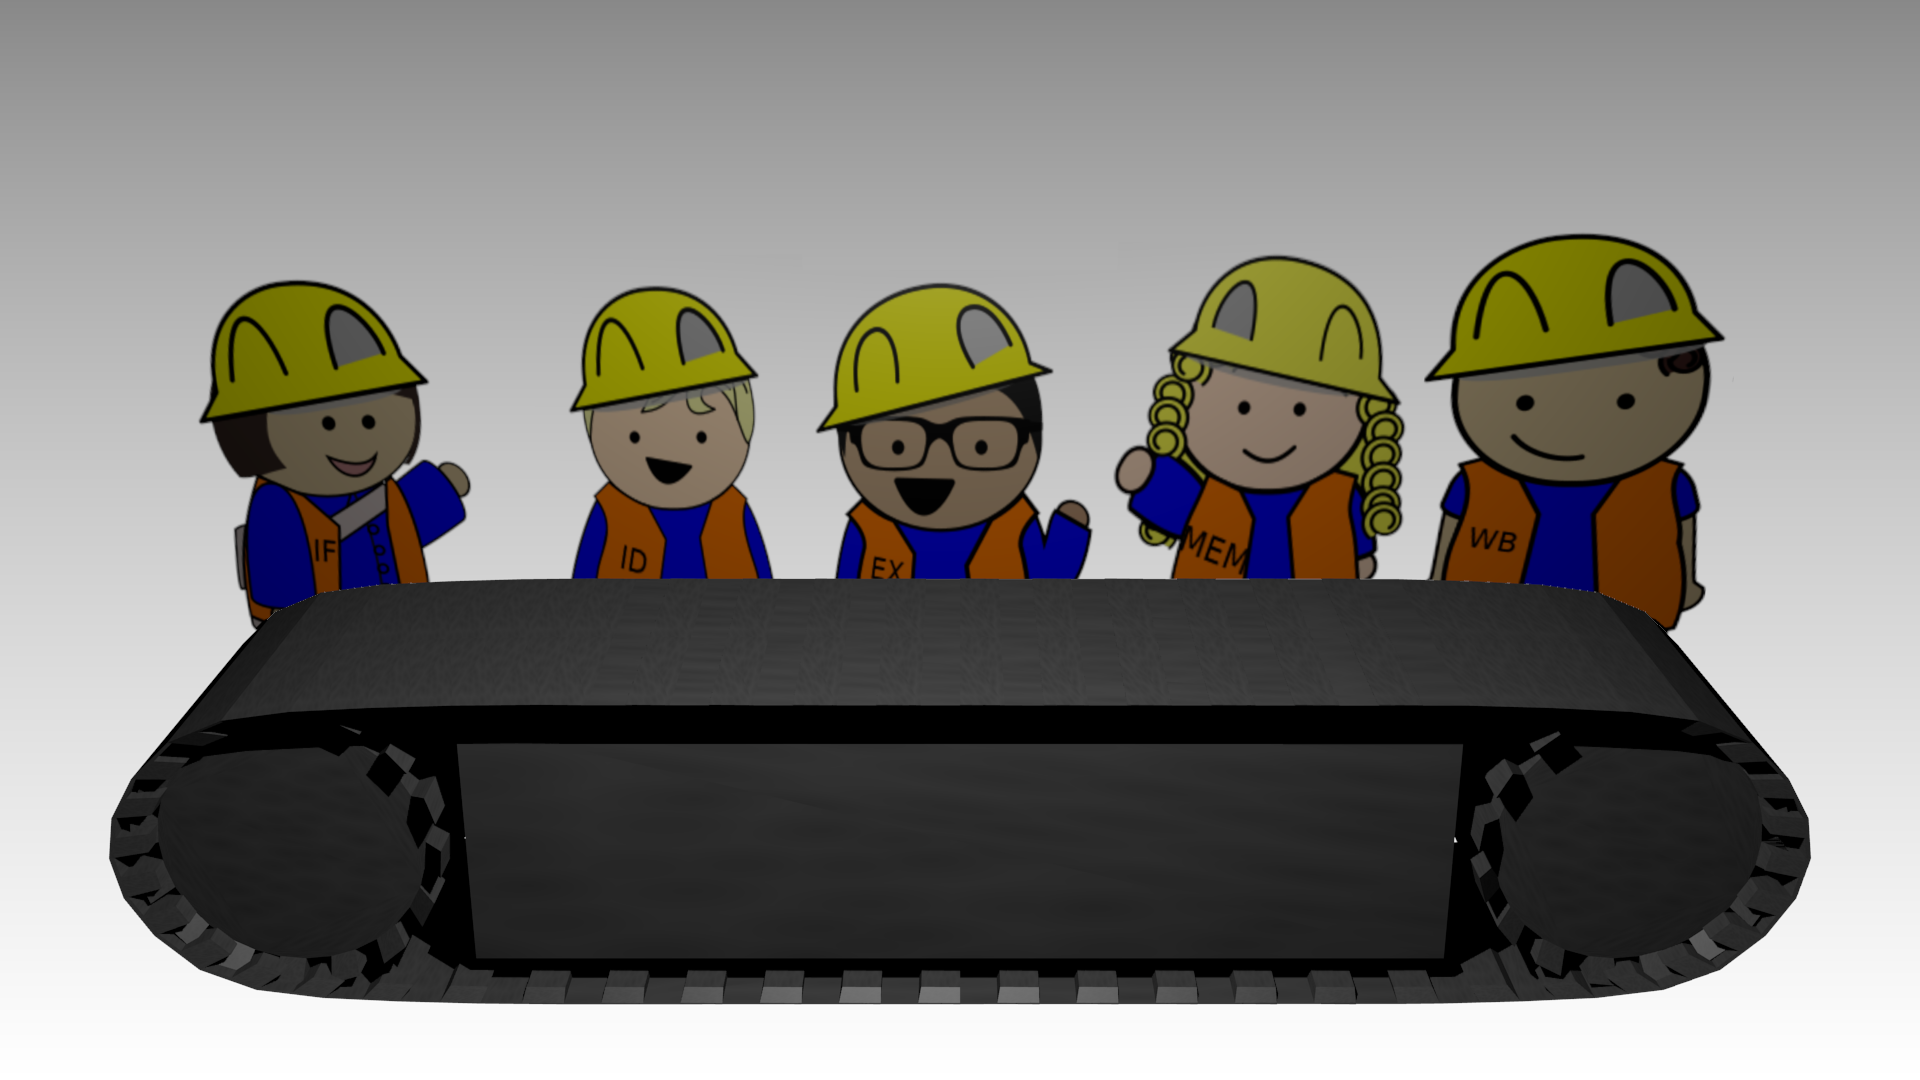
\includegraphics[width=1.0\textwidth]{final.png}}
	%FETCH
	\put(50,-12){\tiny\color{white}7:add t0, t0, 1}
	
	%DECODE
	\put(90,-12){\tiny\color{white}6:nop}
	\put(90,-17){\tiny\color{white}}
	
	%EXECUTE
	\put(135,-12){\tiny\color{white}5:nop}
	\put(135,-17){\tiny\color{white}}
	\put(135,-22){\tiny\color{white}}
	
	%MEMORY
	\put(185,-12){\tiny\color{white}4:add t0, t0, 1}
	\put(185,-17){\tiny\color{white}4:t0 = 1 + 1}
	\put(185,-22){\tiny\color{white}4:t0 = 2}
	
	%WRITEBACK
	\put(225,-12){\tiny\color{white}3:nop}
	\put(225,-17){\tiny\color{white}}
	\put(225,-22){\tiny\color{white}}
	
	%REGISTERS
	\put(80,-37){\tiny\color{white}zero = 0}
	\put(80,-42){\tiny\color{white}ra = 0}
	\put(80,-47){\tiny\color{white}sp = 0}
	\put(80,-52){\tiny\color{white}pc = 28}
	\put(80,-57){\tiny\color{white}t0 = 1}
	\put(80,-62){\tiny\color{white}t1 = 0}
	
	\put(110,-37){\tiny\color{white}t2 = 0}
	\put(110,-42){\tiny\color{white}t3 = 0}
	\put(110,-47){\tiny\color{white}t4 = 0}
	\put(110,-52){\tiny\color{white}t5 = 0}
	\put(110,-57){\tiny\color{white}t6 = 0}
	\put(110,-62){\tiny\color{white}a0 = 0}
	
	\put(140,-37){\tiny\color{white}a1 = 0}
	\put(140,-42){\tiny\color{white}a2 = 0}
	\put(140,-47){\tiny\color{white}a3 = 0}
	\put(140,-52){\tiny\color{white}a4 = 0}
	\put(140,-57){\tiny\color{white}a5 = 0}
	\put(140,-62){\tiny\color{white}a6 = 0}
	
	\put(170,-37){\tiny\color{white}a7 = 0}
	\put(170,-42){\tiny\color{white}s1 = 0}
	\put(170,-47){\tiny\color{white}s2 = 0}
	\put(170,-52){\tiny\color{white}s3 = 0}
	\put(170,-57){\tiny\color{white}s4 = 0}
	\put(170,-62){\tiny\color{white}s5 = 0}
	
	\put(200,-37){\tiny\color{white}s6 = 0}
	\put(200,-42){\tiny\color{white}s7 = 0}
	\put(200,-47){\tiny\color{white}s8 = 0}
	\put(200,-52){\tiny\color{white}s9 = 0}
	\put(200,-57){\tiny\color{white}s10 = 0}
	\put(200,-62){\tiny\color{white}s11 = 0}
	
	\end{picture}
\end{frame}


\begin{frame}
	\frametitle{Pipeline Konfliktlösung: Takt 8}
	\begin{picture}(0,0)
	\put(0,-85){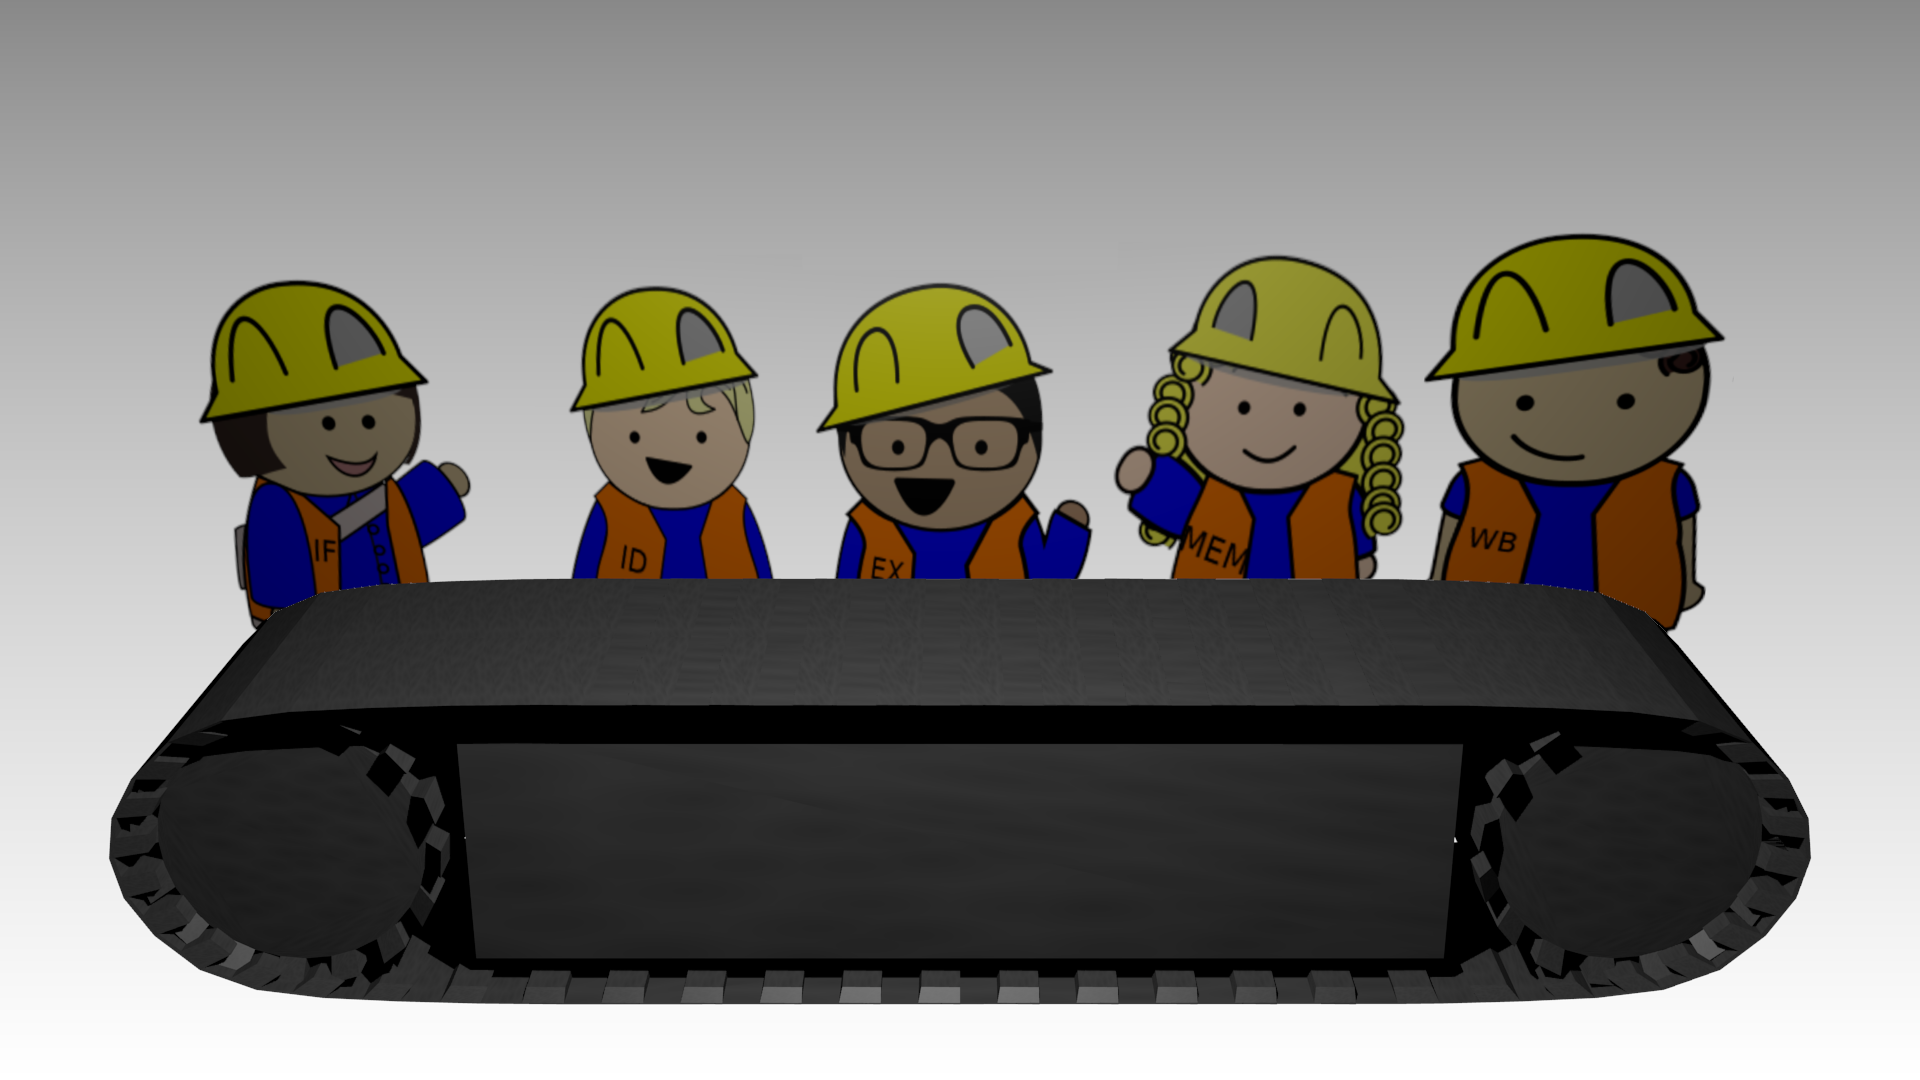
\includegraphics[width=1.0\textwidth]{final.png}}
	%FETCH
	\put(50,-12){\tiny\color{white}8:nop}
	
	%DECODE
	\put(90,-12){\tiny\color{white}7:add t0, t0, 1}
	\put(90,-17){\tiny\color{white}7:t0 = 2 + 1}
	
	%EXECUTE
	\put(135,-12){\tiny\color{white}6:nop}
	\put(135,-17){\tiny\color{white}}
	\put(135,-22){\tiny\color{white}}
	
	%MEMORY
	\put(185,-12){\tiny\color{white}5:nop}
	\put(185,-17){\tiny\color{white}}
	\put(185,-22){\tiny\color{white}}
	
	%WRITEBACK
	\put(225,-12){\tiny\color{white}4:add t0, t0, 1}
	\put(225,-17){\tiny\color{white}4:t0 = 1 + 1}
	\put(225,-22){\tiny\color{white}4:t0 = 2}
	
	%REGISTERS
	\put(80,-37){\tiny\color{white}zero = 0}
	\put(80,-42){\tiny\color{white}ra = 0}
	\put(80,-47){\tiny\color{white}sp = 0}
	\put(80,-52){\tiny\color{white}pc = 32}
	\put(80,-57){\tiny\color{white}t0 = 2}
	\put(80,-62){\tiny\color{white}t1 = 0}
	
	\put(110,-37){\tiny\color{white}t2 = 0}
	\put(110,-42){\tiny\color{white}t3 = 0}
	\put(110,-47){\tiny\color{white}t4 = 0}
	\put(110,-52){\tiny\color{white}t5 = 0}
	\put(110,-57){\tiny\color{white}t6 = 0}
	\put(110,-62){\tiny\color{white}a0 = 0}
	
	\put(140,-37){\tiny\color{white}a1 = 0}
	\put(140,-42){\tiny\color{white}a2 = 0}
	\put(140,-47){\tiny\color{white}a3 = 0}
	\put(140,-52){\tiny\color{white}a4 = 0}
	\put(140,-57){\tiny\color{white}a5 = 0}
	\put(140,-62){\tiny\color{white}a6 = 0}
	
	\put(170,-37){\tiny\color{white}a7 = 0}
	\put(170,-42){\tiny\color{white}s1 = 0}
	\put(170,-47){\tiny\color{white}s2 = 0}
	\put(170,-52){\tiny\color{white}s3 = 0}
	\put(170,-57){\tiny\color{white}s4 = 0}
	\put(170,-62){\tiny\color{white}s5 = 0}
	
	\put(200,-37){\tiny\color{white}s6 = 0}
	\put(200,-42){\tiny\color{white}s7 = 0}
	\put(200,-47){\tiny\color{white}s8 = 0}
	\put(200,-52){\tiny\color{white}s9 = 0}
	\put(200,-57){\tiny\color{white}s10 = 0}
	\put(200,-62){\tiny\color{white}s11 = 0}
	
	\end{picture}
\end{frame}



\begin{frame}
	\frametitle{Pipeline Konfliktlösung: Takt 9}
	\begin{picture}(0,0)
	\put(0,-85){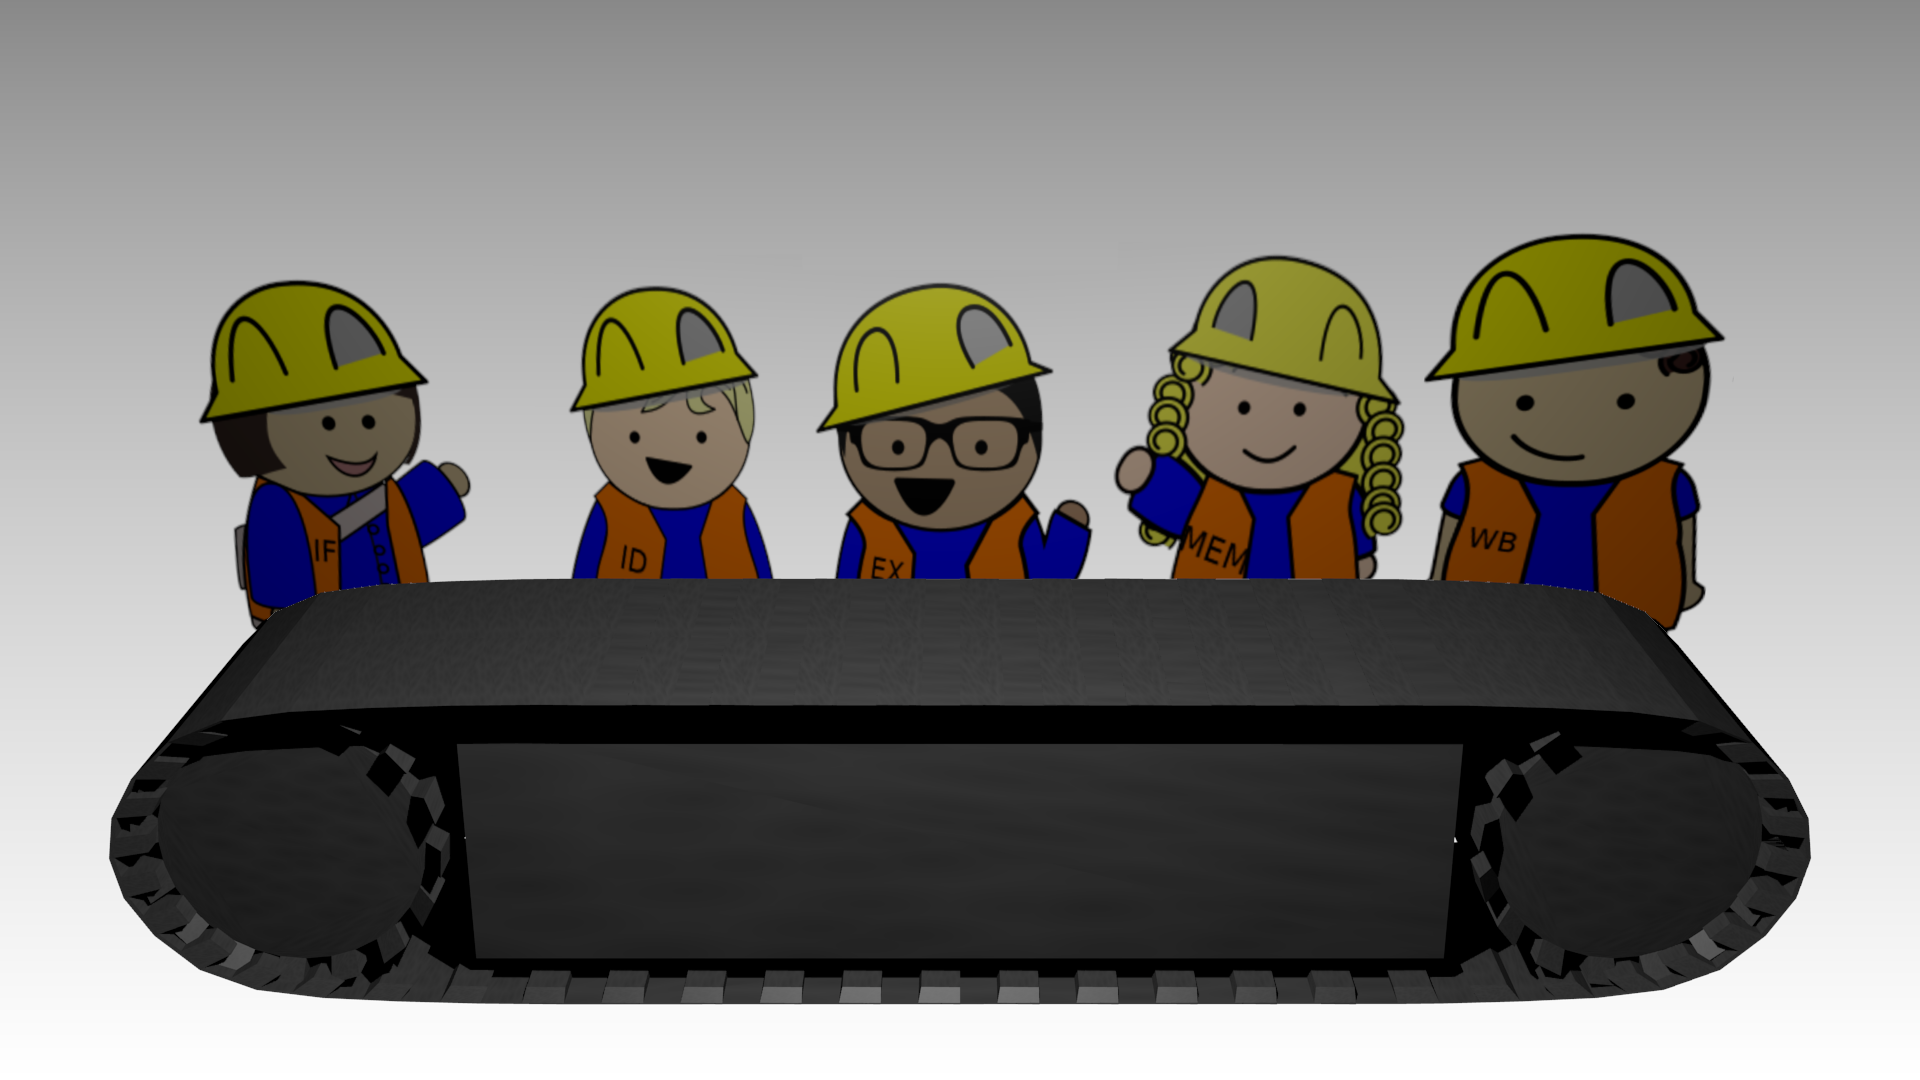
\includegraphics[width=1.0\textwidth]{final.png}}
	%FETCH
	\put(50,-12){\tiny\color{white}9:nop}
	
	%DECODE
	\put(90,-12){\tiny\color{white}8:nop}
	\put(90,-17){\tiny\color{white}}
	
	%EXECUTE
	\put(135,-12){\tiny\color{white}7:add t0, t0, 1}
	\put(135,-17){\tiny\color{white}7:t0 = 2 + 1}
	\put(135,-22){\tiny\color{white}7:t0 = 3}
	
	%MEMORY
	\put(185,-12){\tiny\color{white}6:nop}
	\put(185,-17){\tiny\color{white}}
	\put(185,-22){\tiny\color{white}}
	
	%WRITEBACK
	\put(225,-12){\tiny\color{white}5:nop}
	\put(225,-17){\tiny\color{white}}
	\put(225,-22){\tiny\color{white}}
	
	%REGISTERS
	\put(80,-37){\tiny\color{white}zero = 0}
	\put(80,-42){\tiny\color{white}ra = 0}
	\put(80,-47){\tiny\color{white}sp = 0}
	\put(80,-52){\tiny\color{white}pc = 36}
	\put(80,-57){\tiny\color{white}t0 = 2}
	\put(80,-62){\tiny\color{white}t1 = 0}
	
	\put(110,-37){\tiny\color{white}t2 = 0}
	\put(110,-42){\tiny\color{white}t3 = 0}
	\put(110,-47){\tiny\color{white}t4 = 0}
	\put(110,-52){\tiny\color{white}t5 = 0}
	\put(110,-57){\tiny\color{white}t6 = 0}
	\put(110,-62){\tiny\color{white}a0 = 0}
	
	\put(140,-37){\tiny\color{white}a1 = 0}
	\put(140,-42){\tiny\color{white}a2 = 0}
	\put(140,-47){\tiny\color{white}a3 = 0}
	\put(140,-52){\tiny\color{white}a4 = 0}
	\put(140,-57){\tiny\color{white}a5 = 0}
	\put(140,-62){\tiny\color{white}a6 = 0}
	
	\put(170,-37){\tiny\color{white}a7 = 0}
	\put(170,-42){\tiny\color{white}s1 = 0}
	\put(170,-47){\tiny\color{white}s2 = 0}
	\put(170,-52){\tiny\color{white}s3 = 0}
	\put(170,-57){\tiny\color{white}s4 = 0}
	\put(170,-62){\tiny\color{white}s5 = 0}
	
	\put(200,-37){\tiny\color{white}s6 = 0}
	\put(200,-42){\tiny\color{white}s7 = 0}
	\put(200,-47){\tiny\color{white}s8 = 0}
	\put(200,-52){\tiny\color{white}s9 = 0}
	\put(200,-57){\tiny\color{white}s10 = 0}
	\put(200,-62){\tiny\color{white}s11 = 0}
	
	\end{picture}
\end{frame}


\begin{frame}
	\frametitle{Pipeline Konfliktlösung: Takt 10}
	\begin{picture}(0,0)
	\put(0,-85){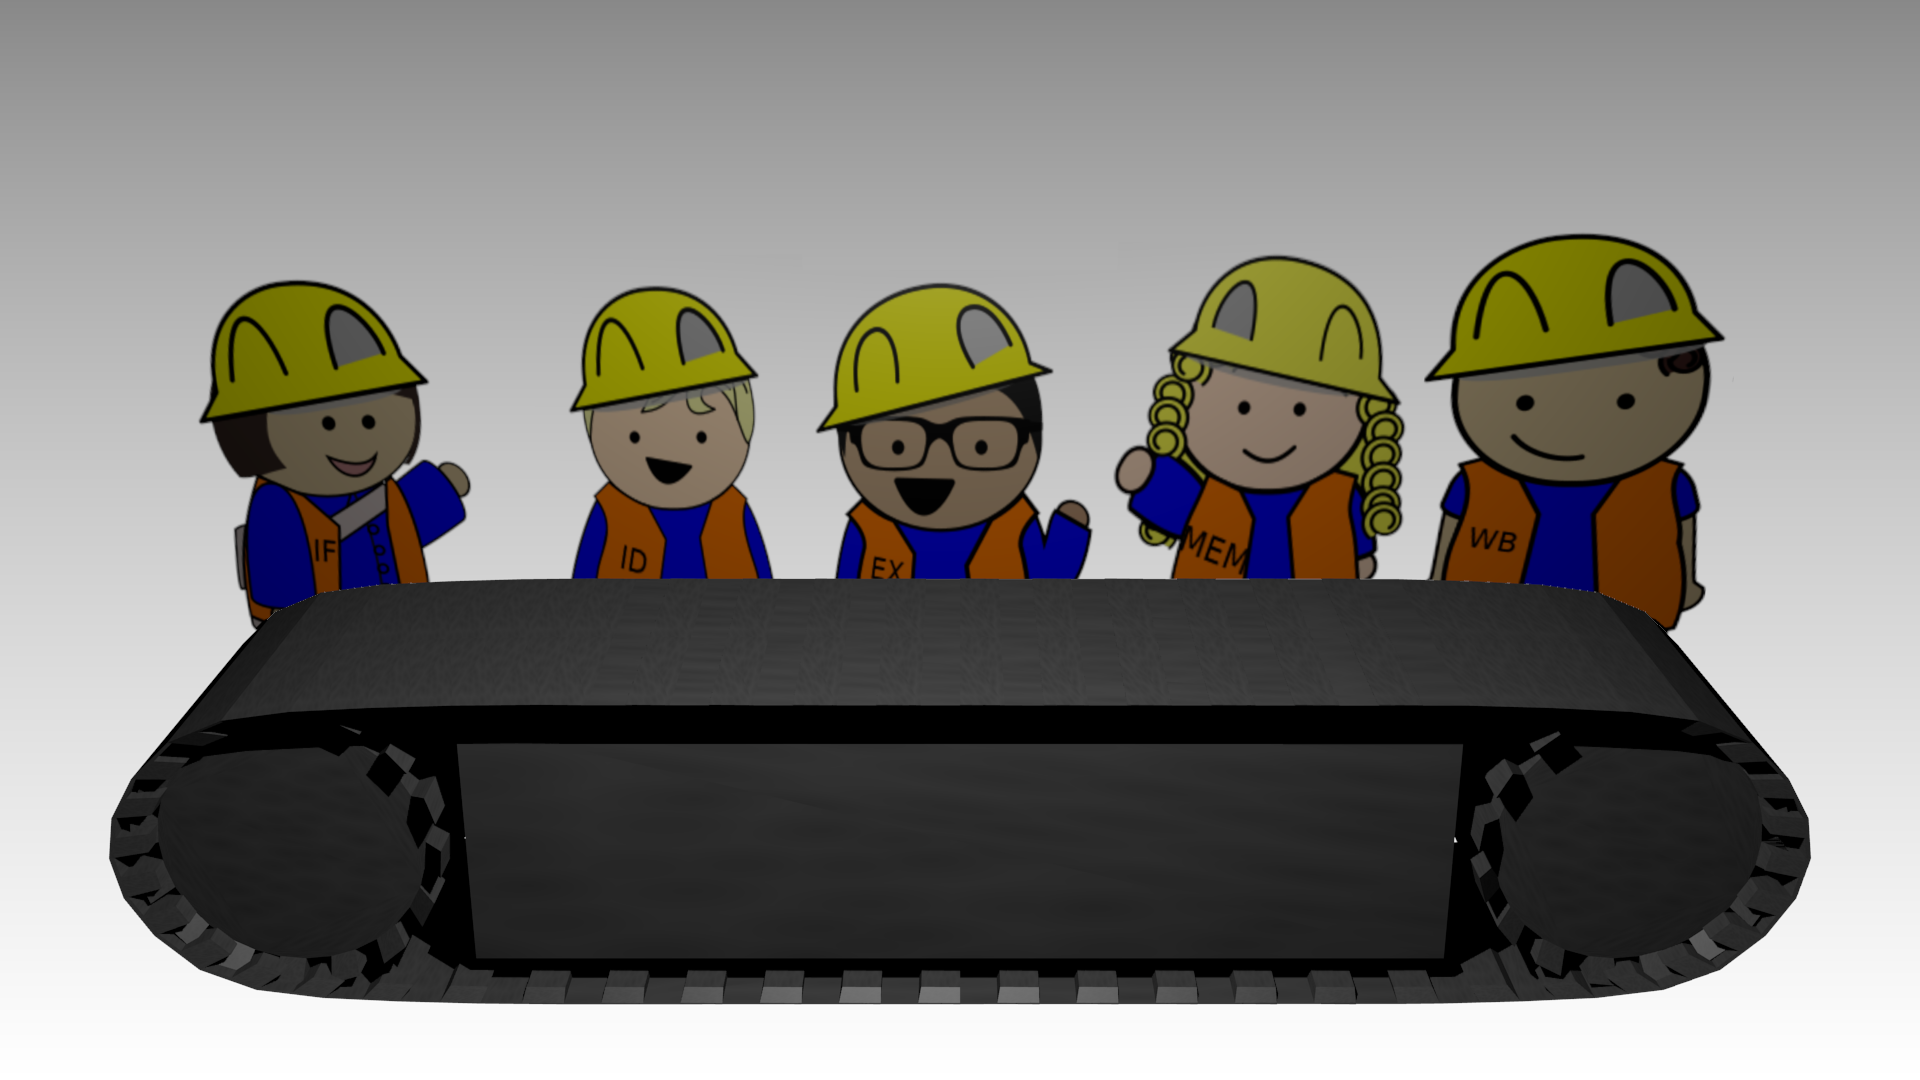
\includegraphics[width=1.0\textwidth]{final.png}}
	%FETCH
	\put(50,-12){\tiny\color{white}10:add t0, t0, 1}
	
	%DECODE
	\put(90,-12){\tiny\color{white}9:nop}
	\put(90,-17){\tiny\color{white}}
	
	%EXECUTE
	\put(135,-12){\tiny\color{white}8:nop}
	\put(135,-17){\tiny\color{white}}
	\put(135,-22){\tiny\color{white}}
	
	%MEMORY
	\put(185,-12){\tiny\color{white}7:add t0, t0, 1}
	\put(185,-17){\tiny\color{white}7:t0 = 2 + 1}
	\put(185,-22){\tiny\color{white}7:t0 = 3}
	
	%WRITEBACK
	\put(225,-12){\tiny\color{white}6:nop}
	\put(225,-17){\tiny\color{white}}
	\put(225,-22){\tiny\color{white}}
	
	%REGISTERS
	\put(80,-37){\tiny\color{white}zero = 0}
	\put(80,-42){\tiny\color{white}ra = 0}
	\put(80,-47){\tiny\color{white}sp = 0}
	\put(80,-52){\tiny\color{white}pc = 40}
	\put(80,-57){\tiny\color{white}t0 = 2}
	\put(80,-62){\tiny\color{white}t1 = 0}
	
	\put(110,-37){\tiny\color{white}t2 = 0}
	\put(110,-42){\tiny\color{white}t3 = 0}
	\put(110,-47){\tiny\color{white}t4 = 0}
	\put(110,-52){\tiny\color{white}t5 = 0}
	\put(110,-57){\tiny\color{white}t6 = 0}
	\put(110,-62){\tiny\color{white}a0 = 0}
	
	\put(140,-37){\tiny\color{white}a1 = 0}
	\put(140,-42){\tiny\color{white}a2 = 0}
	\put(140,-47){\tiny\color{white}a3 = 0}
	\put(140,-52){\tiny\color{white}a4 = 0}
	\put(140,-57){\tiny\color{white}a5 = 0}
	\put(140,-62){\tiny\color{white}a6 = 0}
	
	\put(170,-37){\tiny\color{white}a7 = 0}
	\put(170,-42){\tiny\color{white}s1 = 0}
	\put(170,-47){\tiny\color{white}s2 = 0}
	\put(170,-52){\tiny\color{white}s3 = 0}
	\put(170,-57){\tiny\color{white}s4 = 0}
	\put(170,-62){\tiny\color{white}s5 = 0}
	
	\put(200,-37){\tiny\color{white}s6 = 0}
	\put(200,-42){\tiny\color{white}s7 = 0}
	\put(200,-47){\tiny\color{white}s8 = 0}
	\put(200,-52){\tiny\color{white}s9 = 0}
	\put(200,-57){\tiny\color{white}s10 = 0}
	\put(200,-62){\tiny\color{white}s11 = 0}
	
	\end{picture}
\end{frame}


\begin{frame}
	\frametitle{Pipeline Konfliktlösung: Takt 11}
	\begin{picture}(0,0)
	\put(0,-85){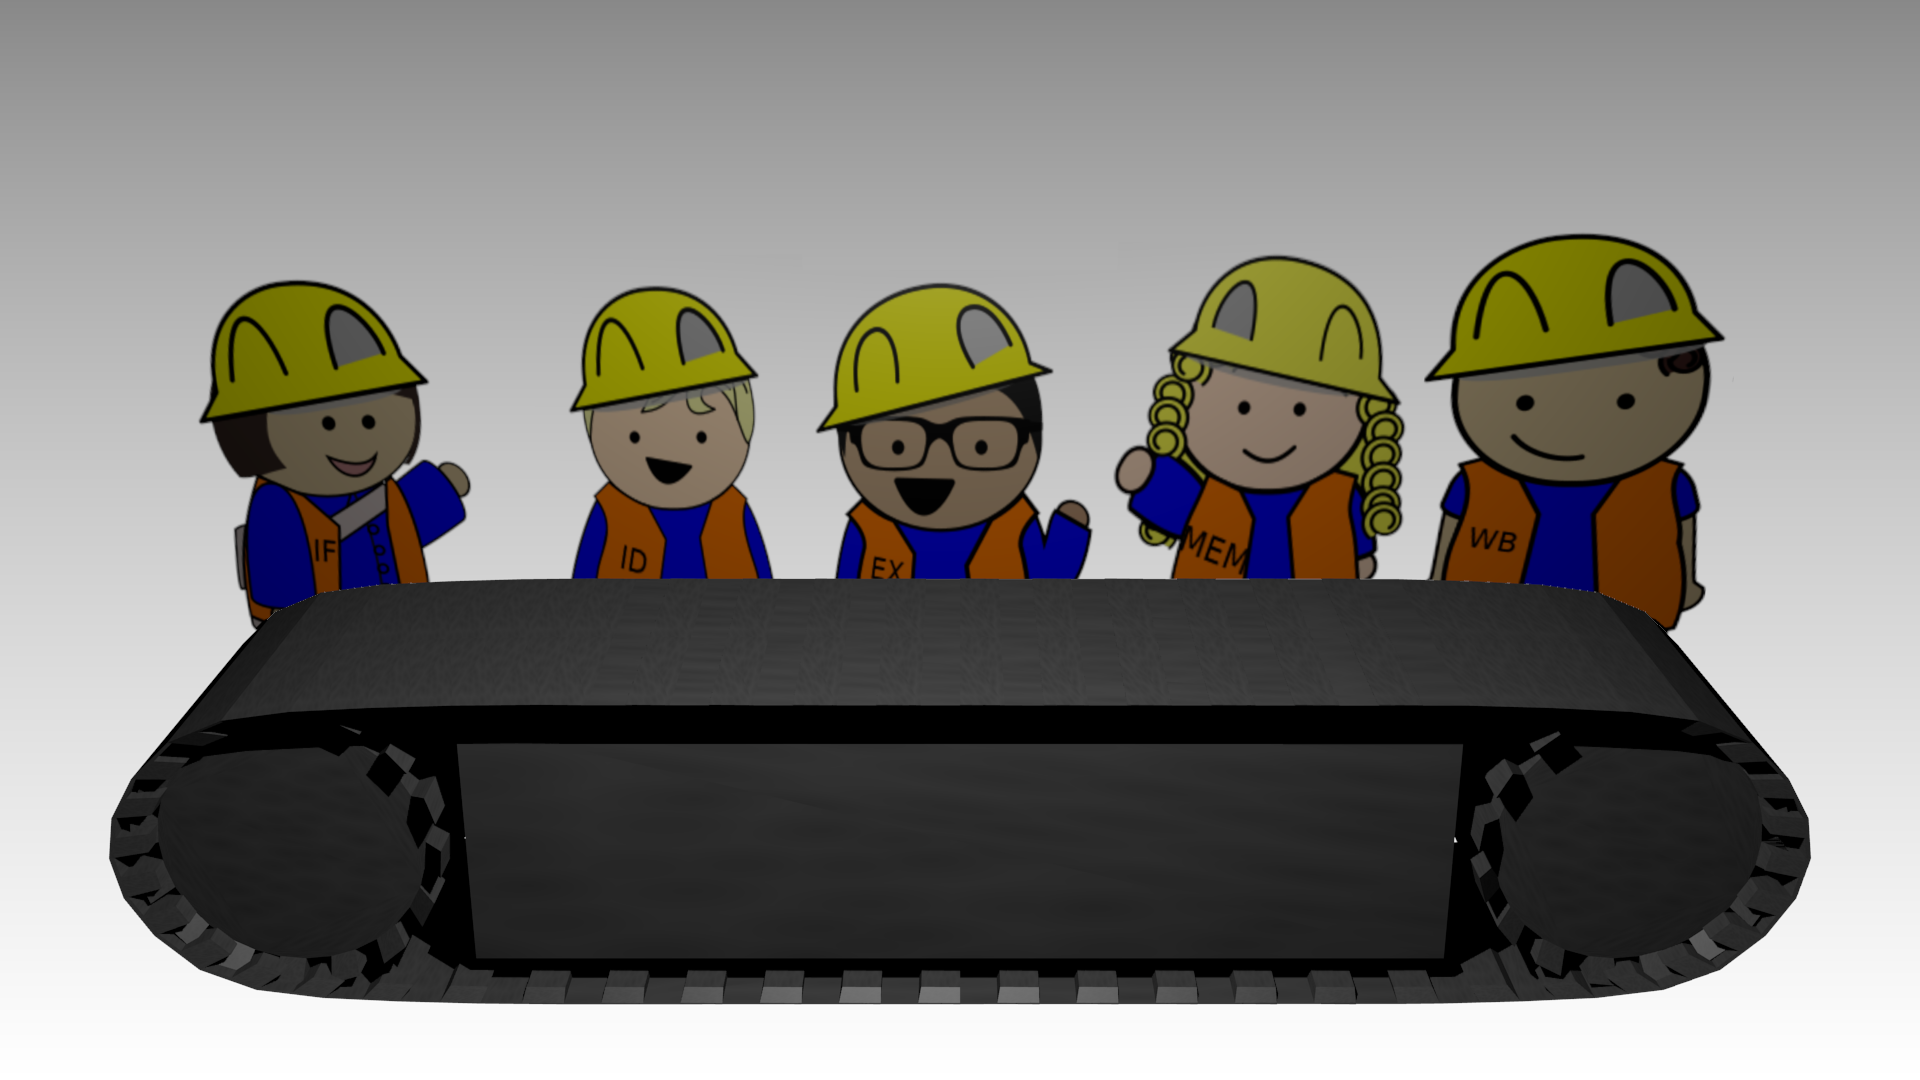
\includegraphics[width=1.0\textwidth]{final.png}}
	%FETCH
	\put(50,-12){\tiny\color{white}11:nop}
	
	%DECODE
	\put(90,-12){\tiny\color{white}10:add t0, t0, 1}
	\put(90,-17){\tiny\color{white}10:t0 = 3 + 1}
	
	%EXECUTE
	\put(135,-12){\tiny\color{white}9:nop}
	\put(135,-17){\tiny\color{white}}
	\put(135,-22){\tiny\color{white}}
	
	%MEMORY
	\put(185,-12){\tiny\color{white}8:nop}
	\put(185,-17){\tiny\color{white}}
	\put(185,-22){\tiny\color{white}}
	
	%WRITEBACK
	\put(225,-12){\tiny\color{white}7:add t0, t0, 1}
	\put(225,-17){\tiny\color{white}7:t0 = 2 + 1}
	\put(225,-22){\tiny\color{white}7:t0 = 3}
	
	%REGISTERS
	\put(80,-37){\tiny\color{white}zero = 0}
	\put(80,-42){\tiny\color{white}ra = 0}
	\put(80,-47){\tiny\color{white}sp = 0}
	\put(80,-52){\tiny\color{white}pc = 44}
	\put(80,-57){\tiny\color{white}t0 = 3}
	\put(80,-62){\tiny\color{white}t1 = 0}
	
	\put(110,-37){\tiny\color{white}t2 = 0}
	\put(110,-42){\tiny\color{white}t3 = 0}
	\put(110,-47){\tiny\color{white}t4 = 0}
	\put(110,-52){\tiny\color{white}t5 = 0}
	\put(110,-57){\tiny\color{white}t6 = 0}
	\put(110,-62){\tiny\color{white}a0 = 0}
	
	\put(140,-37){\tiny\color{white}a1 = 0}
	\put(140,-42){\tiny\color{white}a2 = 0}
	\put(140,-47){\tiny\color{white}a3 = 0}
	\put(140,-52){\tiny\color{white}a4 = 0}
	\put(140,-57){\tiny\color{white}a5 = 0}
	\put(140,-62){\tiny\color{white}a6 = 0}
	
	\put(170,-37){\tiny\color{white}a7 = 0}
	\put(170,-42){\tiny\color{white}s1 = 0}
	\put(170,-47){\tiny\color{white}s2 = 0}
	\put(170,-52){\tiny\color{white}s3 = 0}
	\put(170,-57){\tiny\color{white}s4 = 0}
	\put(170,-62){\tiny\color{white}s5 = 0}
	
	\put(200,-37){\tiny\color{white}s6 = 0}
	\put(200,-42){\tiny\color{white}s7 = 0}
	\put(200,-47){\tiny\color{white}s8 = 0}
	\put(200,-52){\tiny\color{white}s9 = 0}
	\put(200,-57){\tiny\color{white}s10 = 0}
	\put(200,-62){\tiny\color{white}s11 = 0}
	
	\end{picture}
\end{frame}


\begin{frame}
	\frametitle{Pipeline Konfliktlösung: Takt 12}
	\begin{picture}(0,0)
	\put(0,-85){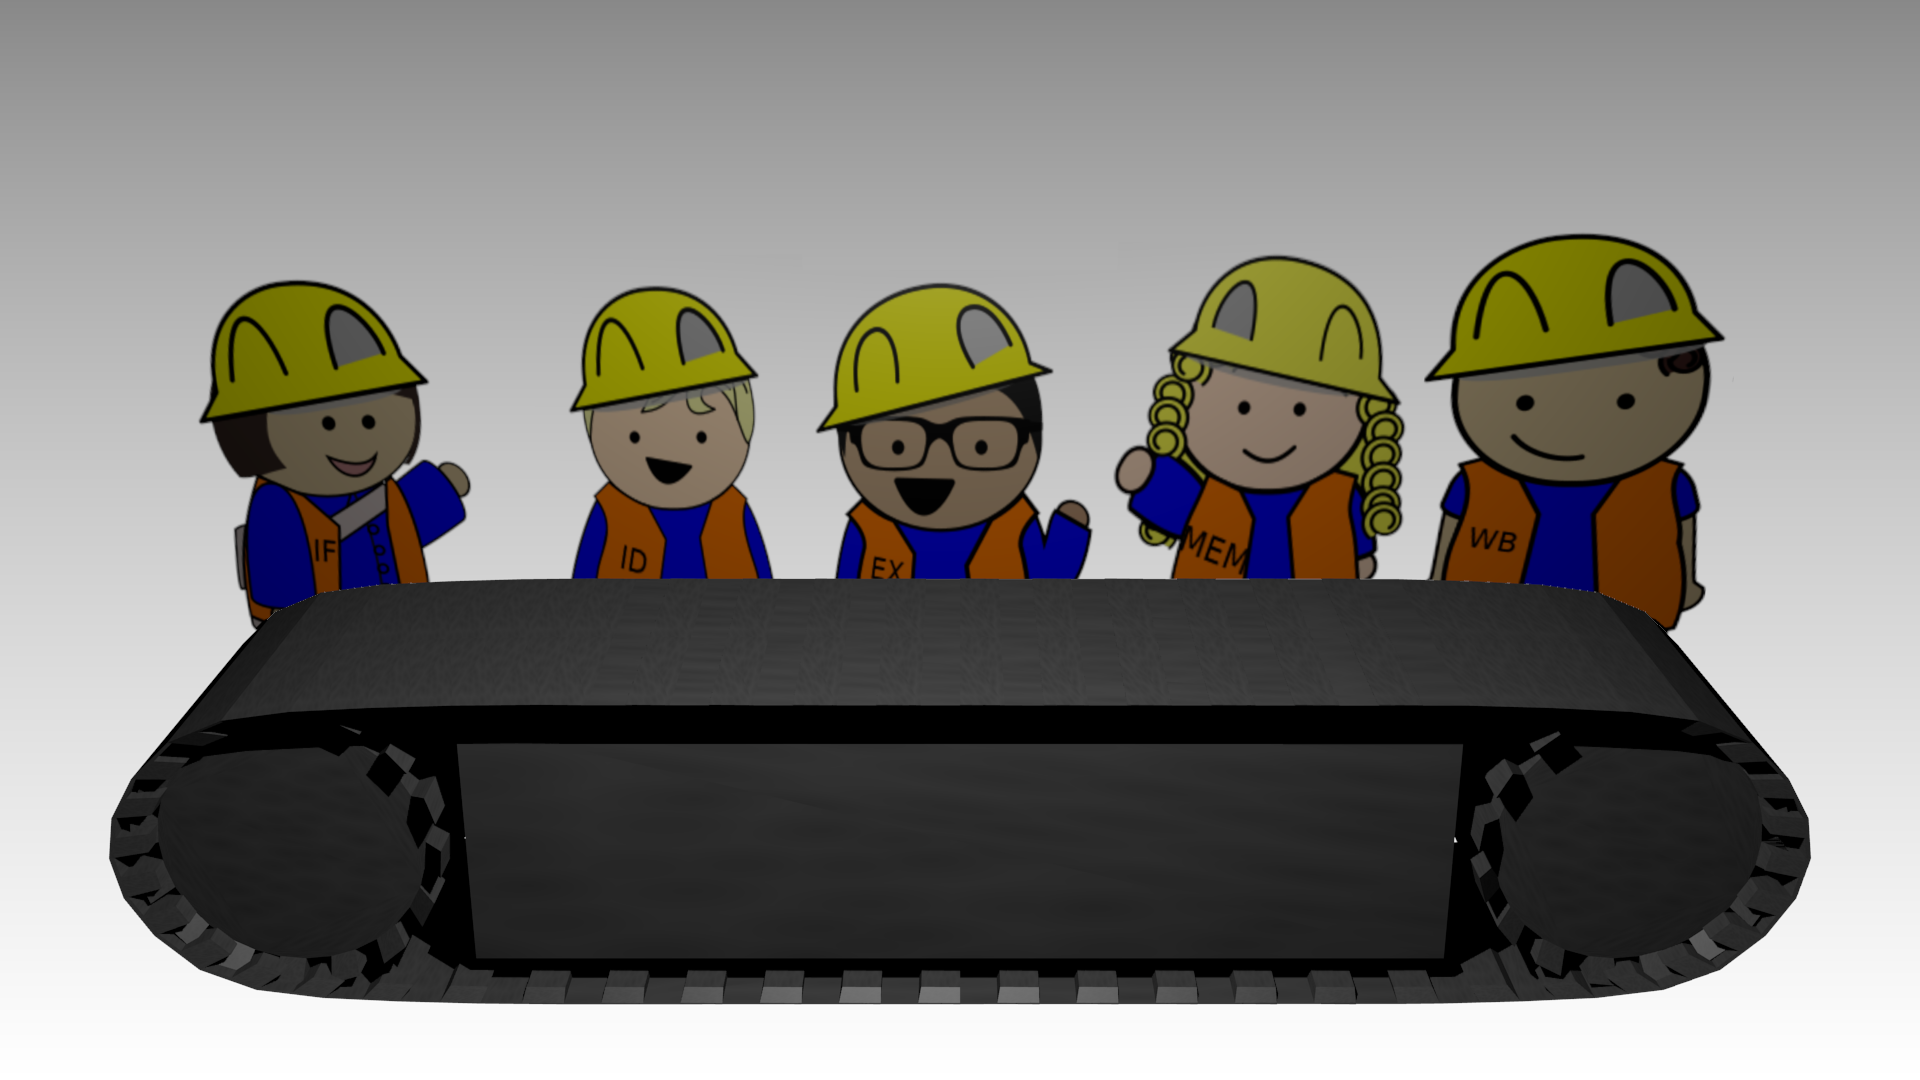
\includegraphics[width=1.0\textwidth]{final.png}}
	%FETCH
	\put(50,-12){\tiny\color{white}12:nop}
	
	%DECODE
	\put(90,-12){\tiny\color{white}11:nop}
	\put(90,-17){\tiny\color{white}}
	
	%EXECUTE
	\put(135,-12){\tiny\color{white}10:add t0, t0, 1}
	\put(135,-17){\tiny\color{white}10:t0 = 3 + 1}
	\put(135,-22){\tiny\color{white}10:t0 = 4}
	
	%MEMORY
	\put(185,-12){\tiny\color{white}9:nop}
	\put(185,-17){\tiny\color{white}}
	\put(185,-22){\tiny\color{white}}
	
	%WRITEBACK
	\put(225,-12){\tiny\color{white}8:nop}
	\put(225,-17){\tiny\color{white}}
	\put(225,-22){\tiny\color{white}}
	
	%REGISTERS
	\put(80,-37){\tiny\color{white}zero = 0}
	\put(80,-42){\tiny\color{white}ra = 0}
	\put(80,-47){\tiny\color{white}sp = 0}
	\put(80,-52){\tiny\color{white}pc = 48}
	\put(80,-57){\tiny\color{white}t0 = 3}
	\put(80,-62){\tiny\color{white}t1 = 0}
	
	\put(110,-37){\tiny\color{white}t2 = 0}
	\put(110,-42){\tiny\color{white}t3 = 0}
	\put(110,-47){\tiny\color{white}t4 = 0}
	\put(110,-52){\tiny\color{white}t5 = 0}
	\put(110,-57){\tiny\color{white}t6 = 0}
	\put(110,-62){\tiny\color{white}a0 = 0}
	
	\put(140,-37){\tiny\color{white}a1 = 0}
	\put(140,-42){\tiny\color{white}a2 = 0}
	\put(140,-47){\tiny\color{white}a3 = 0}
	\put(140,-52){\tiny\color{white}a4 = 0}
	\put(140,-57){\tiny\color{white}a5 = 0}
	\put(140,-62){\tiny\color{white}a6 = 0}
	
	\put(170,-37){\tiny\color{white}a7 = 0}
	\put(170,-42){\tiny\color{white}s1 = 0}
	\put(170,-47){\tiny\color{white}s2 = 0}
	\put(170,-52){\tiny\color{white}s3 = 0}
	\put(170,-57){\tiny\color{white}s4 = 0}
	\put(170,-62){\tiny\color{white}s5 = 0}
	
	\put(200,-37){\tiny\color{white}s6 = 0}
	\put(200,-42){\tiny\color{white}s7 = 0}
	\put(200,-47){\tiny\color{white}s8 = 0}
	\put(200,-52){\tiny\color{white}s9 = 0}
	\put(200,-57){\tiny\color{white}s10 = 0}
	\put(200,-62){\tiny\color{white}s11 = 0}
	
	\end{picture}
\end{frame}


\begin{frame}
	\frametitle{Pipeline Konfliktlösung: Takt 13}
	\begin{picture}(0,0)
	\put(0,-85){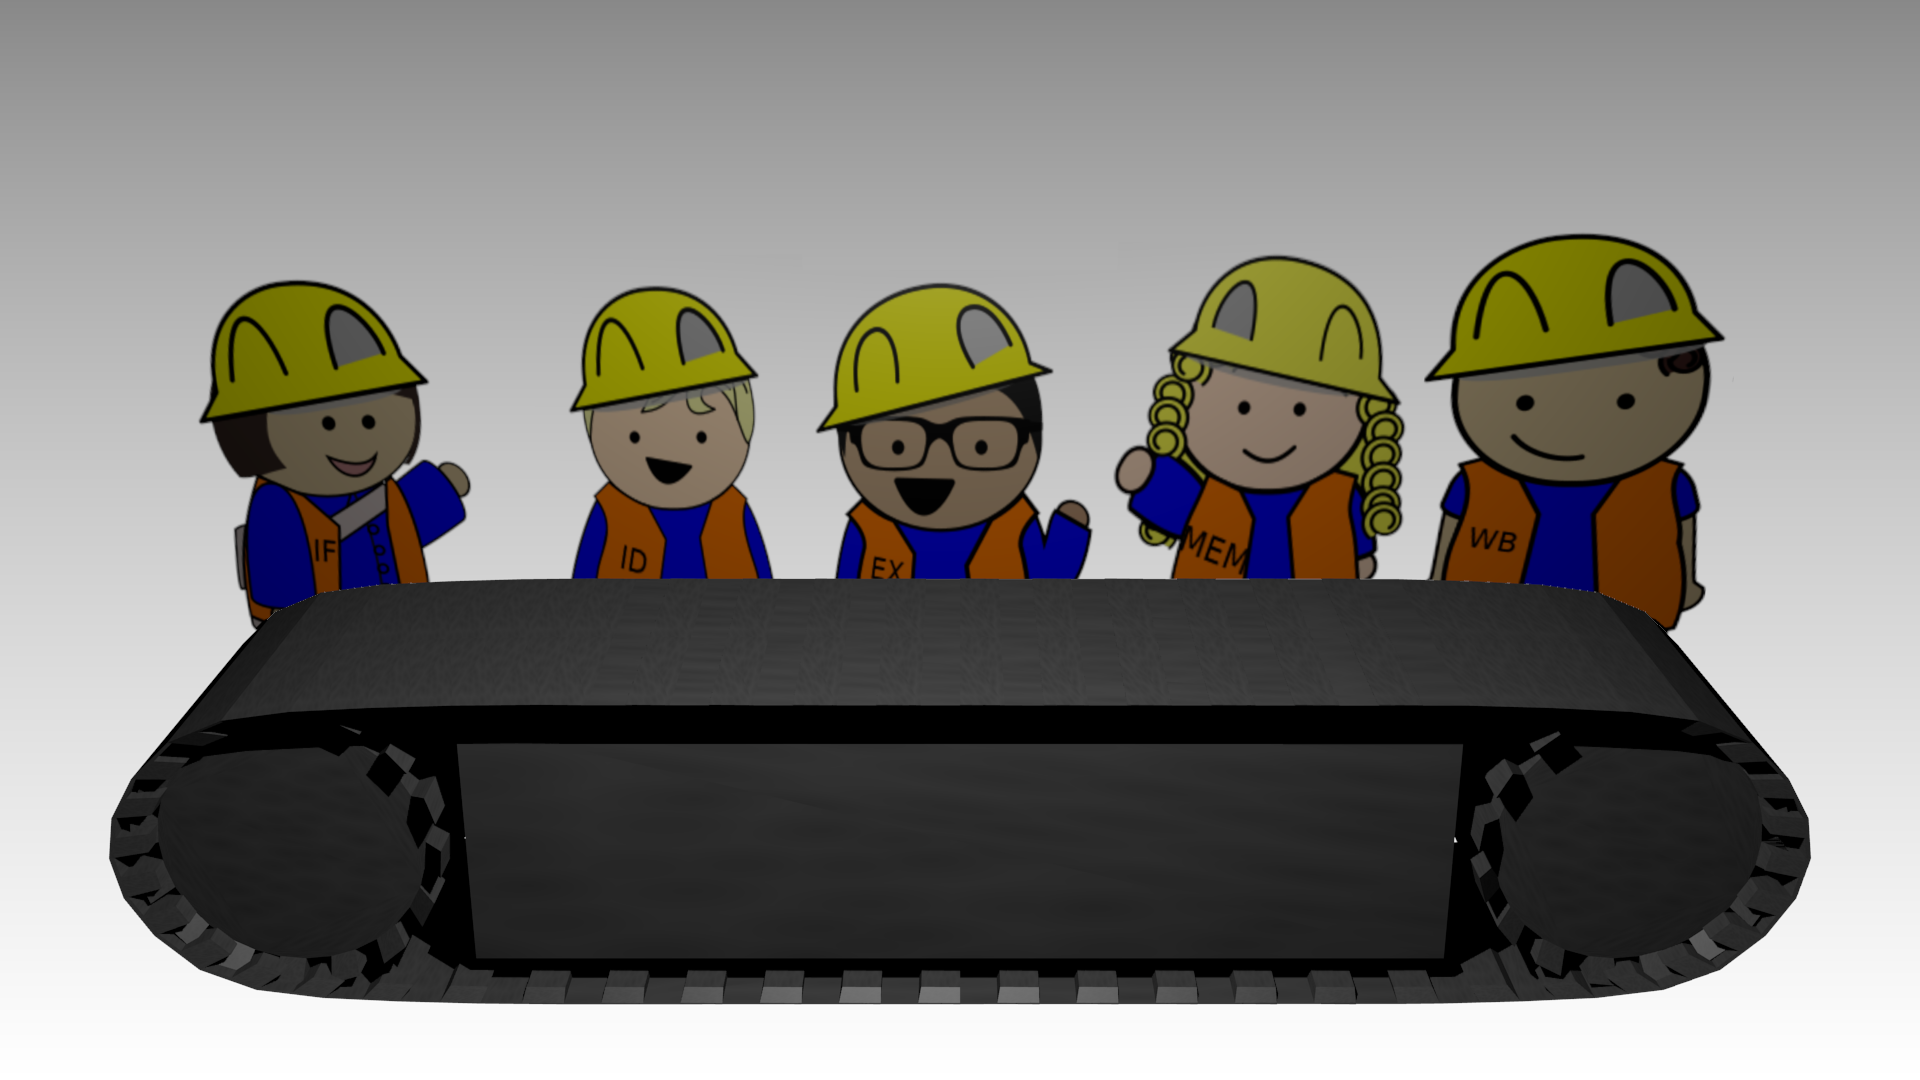
\includegraphics[width=1.0\textwidth]{final.png}}
	%FETCH
	\put(50,-12){\tiny\color{white}13:add t0, t0, 1}
	
	%DECODE
	\put(90,-12){\tiny\color{white}12:nop}
	\put(90,-17){\tiny\color{white}}
	
	%EXECUTE
	\put(135,-12){\tiny\color{white}11:nop}
	\put(135,-17){\tiny\color{white}}
	\put(135,-22){\tiny\color{white}}
	
	%MEMORY
	\put(185,-12){\tiny\color{white}10:add t0, t0, 1}
	\put(185,-17){\tiny\color{white}10:t0 = 3 + 1}
	\put(185,-22){\tiny\color{white}10:t0 = 4}
	
	%WRITEBACK
	\put(225,-12){\tiny\color{white}9:nop}
	\put(225,-17){\tiny\color{white}}
	\put(225,-22){\tiny\color{white}}
	
	%REGISTERS
	\put(80,-37){\tiny\color{white}zero = 0}
	\put(80,-42){\tiny\color{white}ra = 0}
	\put(80,-47){\tiny\color{white}sp = 0}
	\put(80,-52){\tiny\color{white}pc = 52}
	\put(80,-57){\tiny\color{white}t0 = 3}
	\put(80,-62){\tiny\color{white}t1 = 0}
	
	\put(110,-37){\tiny\color{white}t2 = 0}
	\put(110,-42){\tiny\color{white}t3 = 0}
	\put(110,-47){\tiny\color{white}t4 = 0}
	\put(110,-52){\tiny\color{white}t5 = 0}
	\put(110,-57){\tiny\color{white}t6 = 0}
	\put(110,-62){\tiny\color{white}a0 = 0}
	
	\put(140,-37){\tiny\color{white}a1 = 0}
	\put(140,-42){\tiny\color{white}a2 = 0}
	\put(140,-47){\tiny\color{white}a3 = 0}
	\put(140,-52){\tiny\color{white}a4 = 0}
	\put(140,-57){\tiny\color{white}a5 = 0}
	\put(140,-62){\tiny\color{white}a6 = 0}
	
	\put(170,-37){\tiny\color{white}a7 = 0}
	\put(170,-42){\tiny\color{white}s1 = 0}
	\put(170,-47){\tiny\color{white}s2 = 0}
	\put(170,-52){\tiny\color{white}s3 = 0}
	\put(170,-57){\tiny\color{white}s4 = 0}
	\put(170,-62){\tiny\color{white}s5 = 0}
	
	\put(200,-37){\tiny\color{white}s6 = 0}
	\put(200,-42){\tiny\color{white}s7 = 0}
	\put(200,-47){\tiny\color{white}s8 = 0}
	\put(200,-52){\tiny\color{white}s9 = 0}
	\put(200,-57){\tiny\color{white}s10 = 0}
	\put(200,-62){\tiny\color{white}s11 = 0}
	
	\end{picture}
\end{frame}


\begin{frame}
	\frametitle{Pipeline Konfliktlösung: Takt 14}
	\begin{picture}(0,0)
	\put(0,-85){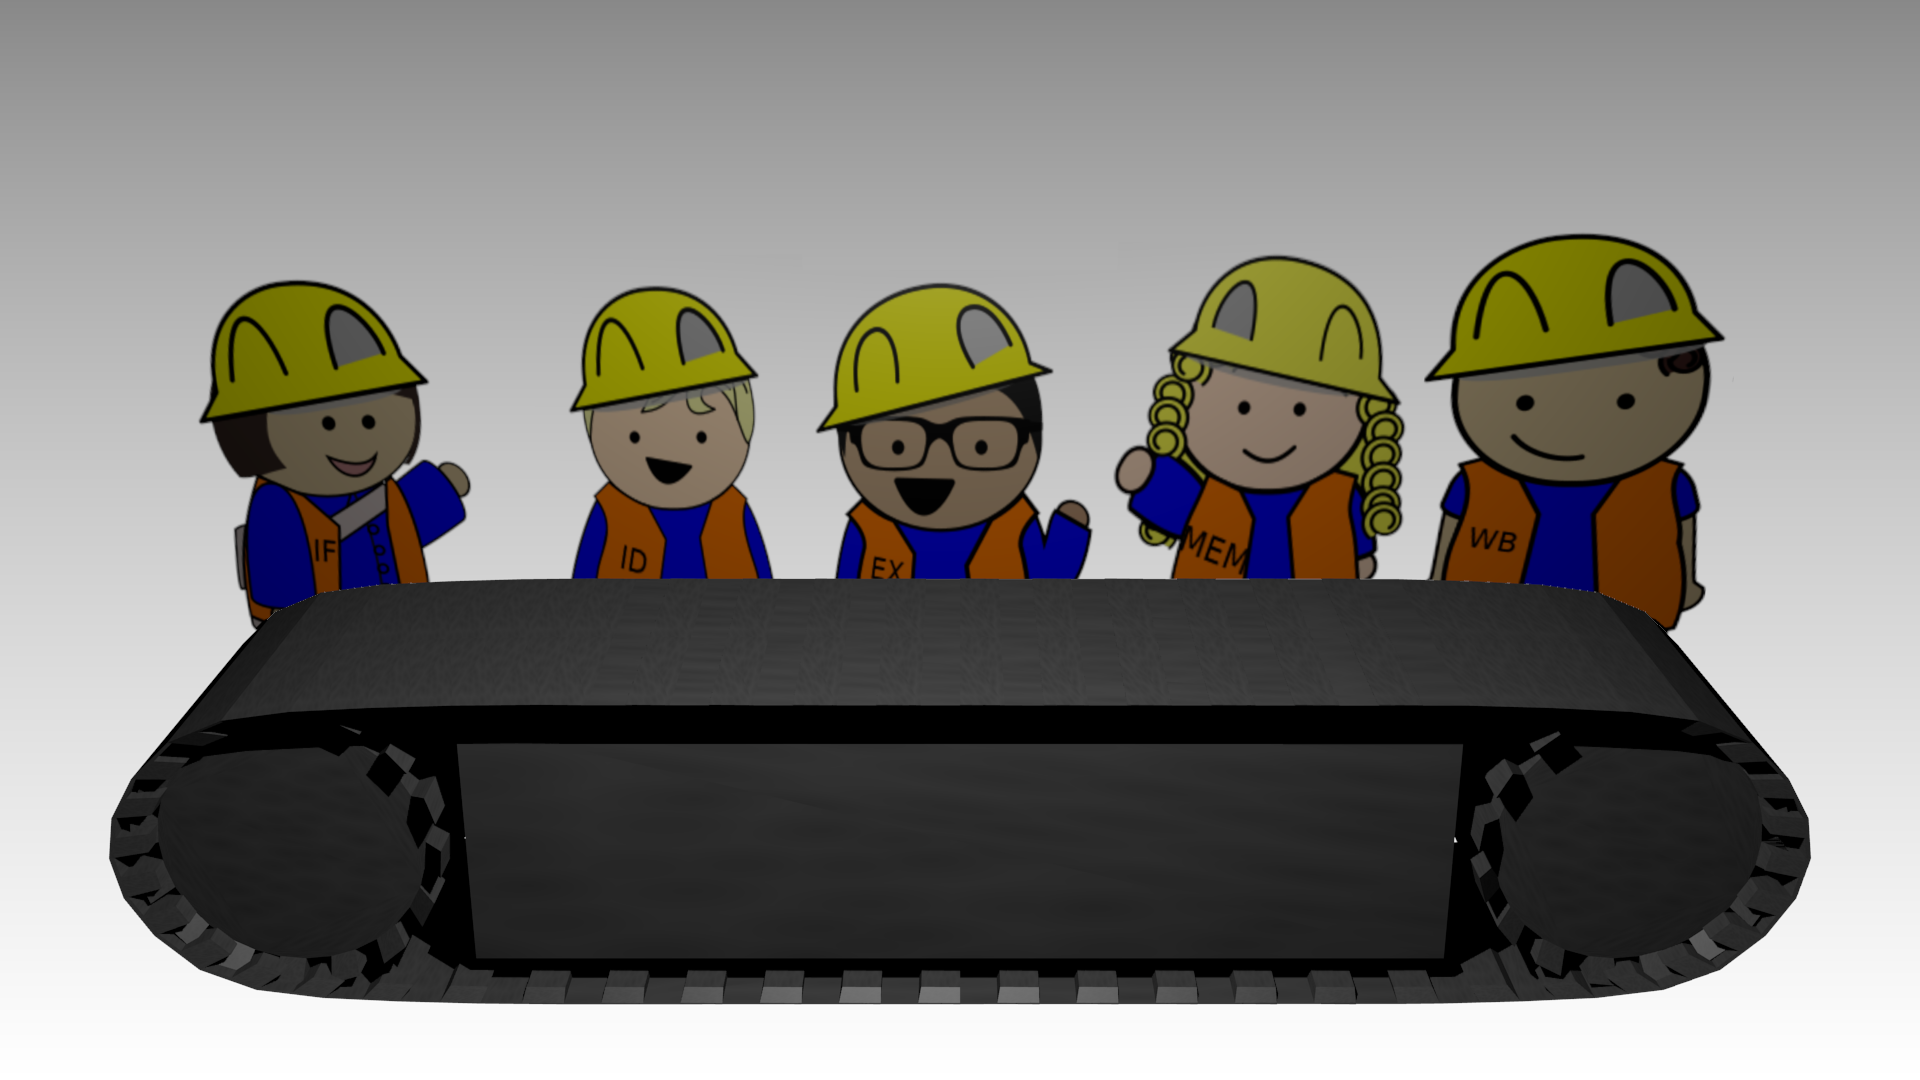
\includegraphics[width=1.0\textwidth]{final.png}}
	%FETCH
	\put(50,-12){\tiny\color{white}}
	
	%DECODE
	\put(90,-12){\tiny\color{white}13:add t0, t0, 1}
	\put(90,-17){\tiny\color{white}13:t0 = 4 + 1}
	
	%EXECUTE
	\put(135,-12){\tiny\color{white}12:nop}
	\put(135,-17){\tiny\color{white}}
	\put(135,-22){\tiny\color{white}}
	
	%MEMORY
	\put(185,-12){\tiny\color{white}11:nop}
	\put(185,-17){\tiny\color{white}}
	\put(185,-22){\tiny\color{white}}
	
	%WRITEBACK
	\put(225,-12){\tiny\color{white}10:add t0, t0, 1}
	\put(225,-17){\tiny\color{white}10:t0 = 3 + 1}
	\put(225,-22){\tiny\color{white}10:t0 = 4}
	
	%REGISTERS
	\put(80,-37){\tiny\color{white}zero = 0}
	\put(80,-42){\tiny\color{white}ra = 0}
	\put(80,-47){\tiny\color{white}sp = 0}
	\put(80,-52){\tiny\color{white}pc = 56}
	\put(80,-57){\tiny\color{white}t0 = 4}
	\put(80,-62){\tiny\color{white}t1 = 0}
	
	\put(110,-37){\tiny\color{white}t2 = 0}
	\put(110,-42){\tiny\color{white}t3 = 0}
	\put(110,-47){\tiny\color{white}t4 = 0}
	\put(110,-52){\tiny\color{white}t5 = 0}
	\put(110,-57){\tiny\color{white}t6 = 0}
	\put(110,-62){\tiny\color{white}a0 = 0}
	
	\put(140,-37){\tiny\color{white}a1 = 0}
	\put(140,-42){\tiny\color{white}a2 = 0}
	\put(140,-47){\tiny\color{white}a3 = 0}
	\put(140,-52){\tiny\color{white}a4 = 0}
	\put(140,-57){\tiny\color{white}a5 = 0}
	\put(140,-62){\tiny\color{white}a6 = 0}
	
	\put(170,-37){\tiny\color{white}a7 = 0}
	\put(170,-42){\tiny\color{white}s1 = 0}
	\put(170,-47){\tiny\color{white}s2 = 0}
	\put(170,-52){\tiny\color{white}s3 = 0}
	\put(170,-57){\tiny\color{white}s4 = 0}
	\put(170,-62){\tiny\color{white}s5 = 0}
	
	\put(200,-37){\tiny\color{white}s6 = 0}
	\put(200,-42){\tiny\color{white}s7 = 0}
	\put(200,-47){\tiny\color{white}s8 = 0}
	\put(200,-52){\tiny\color{white}s9 = 0}
	\put(200,-57){\tiny\color{white}s10 = 0}
	\put(200,-62){\tiny\color{white}s11 = 0}
	
	\end{picture}
\end{frame}


\begin{frame}
	\frametitle{Pipeline Konfliktlösung: Takt 15}
	\begin{picture}(0,0)
	\put(0,-85){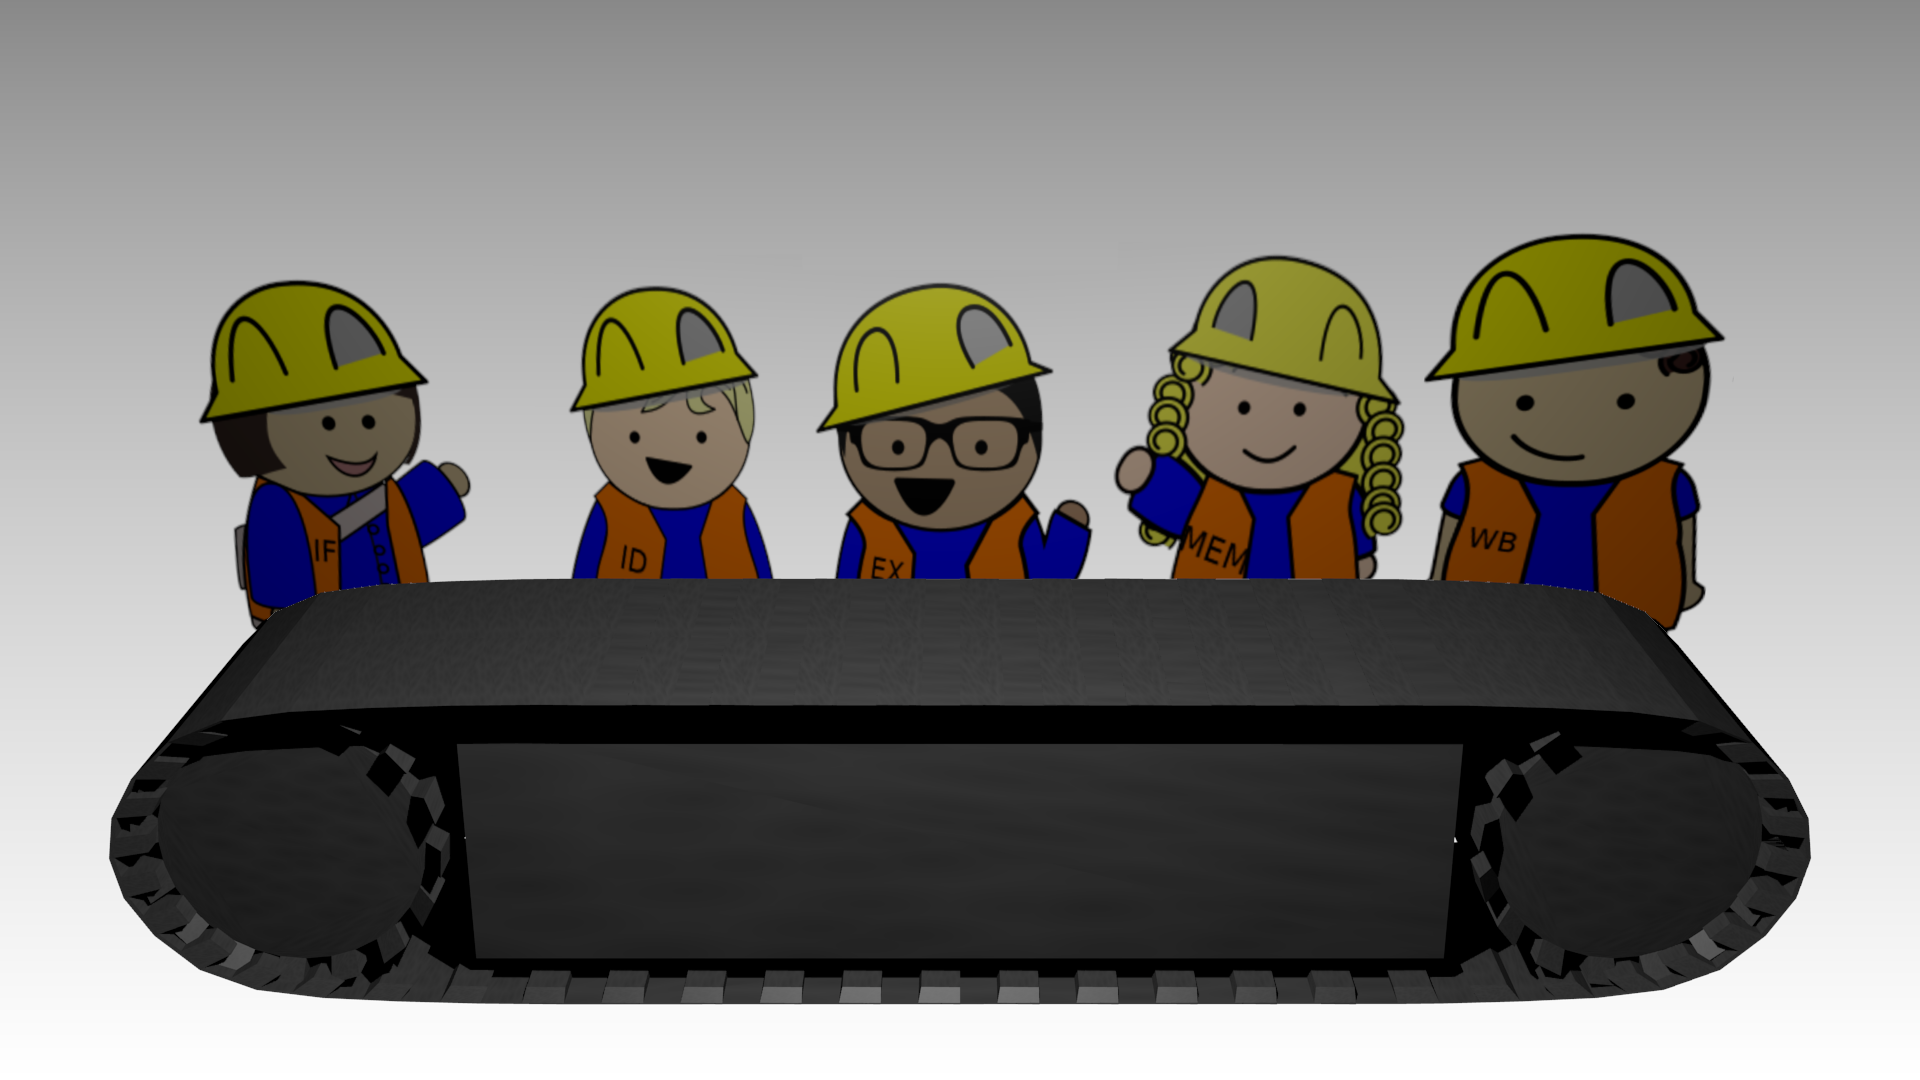
\includegraphics[width=1.0\textwidth]{final.png}}
	%FETCH
	\put(50,-12){\tiny\color{white}}
	
	%DECODE
	\put(90,-12){\tiny\color{white}}
	\put(90,-17){\tiny\color{white}}
	
	%EXECUTE
	\put(135,-12){\tiny\color{white}13:add t0, t0, 1}
	\put(135,-17){\tiny\color{white}13:t0 = 4 + 1}
	\put(135,-22){\tiny\color{white}13:t0 = 5}
	
	%MEMORY
	\put(185,-12){\tiny\color{white}12:nop}
	\put(185,-17){\tiny\color{white}}
	\put(185,-22){\tiny\color{white}}
	
	%WRITEBACK
	\put(225,-12){\tiny\color{white}11:nop}
	\put(225,-17){\tiny\color{white}}
	\put(225,-22){\tiny\color{white}}
	
	%REGISTERS
	\put(80,-37){\tiny\color{white}zero = 0}
	\put(80,-42){\tiny\color{white}ra = 0}
	\put(80,-47){\tiny\color{white}sp = 0}
	\put(80,-52){\tiny\color{white}pc = 60}
	\put(80,-57){\tiny\color{white}t0 = 4}
	\put(80,-62){\tiny\color{white}t1 = 0}
	
	\put(110,-37){\tiny\color{white}t2 = 0}
	\put(110,-42){\tiny\color{white}t3 = 0}
	\put(110,-47){\tiny\color{white}t4 = 0}
	\put(110,-52){\tiny\color{white}t5 = 0}
	\put(110,-57){\tiny\color{white}t6 = 0}
	\put(110,-62){\tiny\color{white}a0 = 0}
	
	\put(140,-37){\tiny\color{white}a1 = 0}
	\put(140,-42){\tiny\color{white}a2 = 0}
	\put(140,-47){\tiny\color{white}a3 = 0}
	\put(140,-52){\tiny\color{white}a4 = 0}
	\put(140,-57){\tiny\color{white}a5 = 0}
	\put(140,-62){\tiny\color{white}a6 = 0}
	
	\put(170,-37){\tiny\color{white}a7 = 0}
	\put(170,-42){\tiny\color{white}s1 = 0}
	\put(170,-47){\tiny\color{white}s2 = 0}
	\put(170,-52){\tiny\color{white}s3 = 0}
	\put(170,-57){\tiny\color{white}s4 = 0}
	\put(170,-62){\tiny\color{white}s5 = 0}
	
	\put(200,-37){\tiny\color{white}s6 = 0}
	\put(200,-42){\tiny\color{white}s7 = 0}
	\put(200,-47){\tiny\color{white}s8 = 0}
	\put(200,-52){\tiny\color{white}s9 = 0}
	\put(200,-57){\tiny\color{white}s10 = 0}
	\put(200,-62){\tiny\color{white}s11 = 0}
	
	\end{picture}
\end{frame}



\begin{frame}
	\frametitle{Pipeline Konfliktlösung: Takt 16}
	\begin{picture}(0,0)
	\put(0,-85){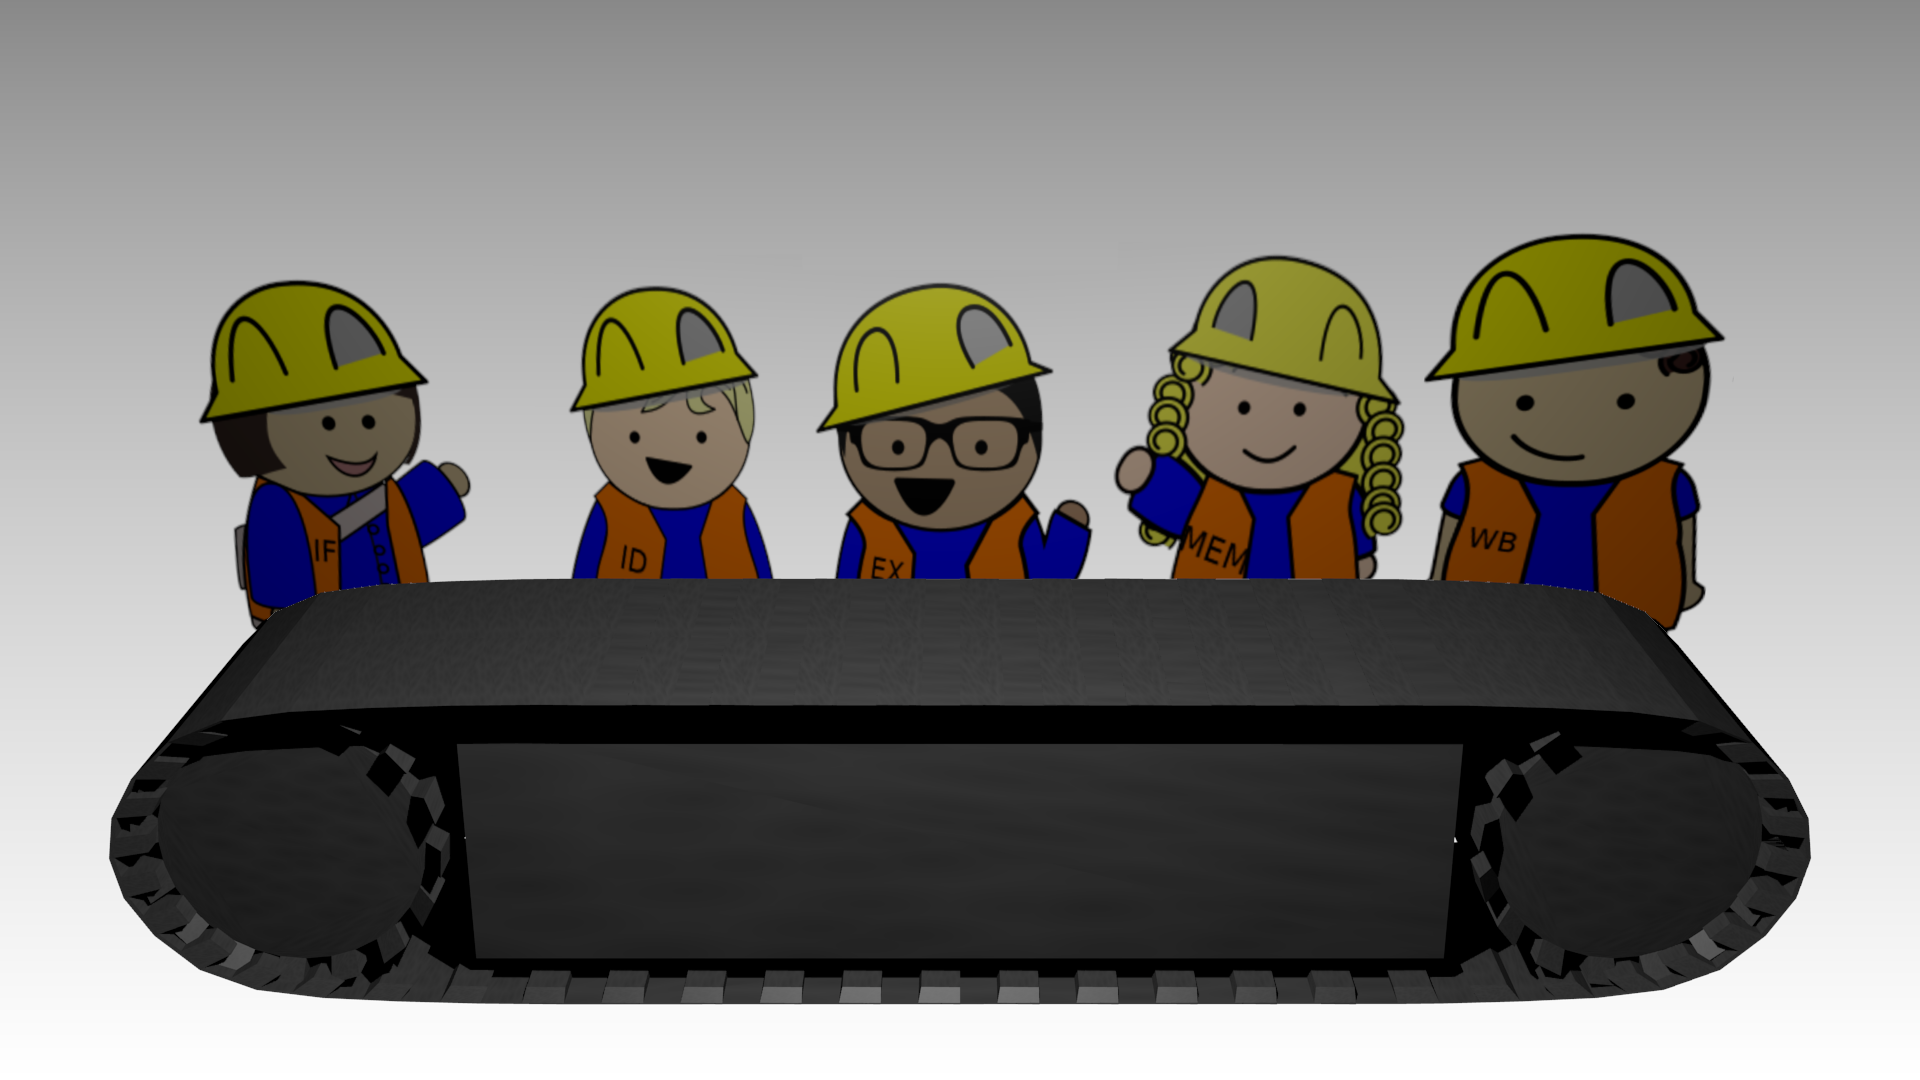
\includegraphics[width=1.0\textwidth]{final.png}}
	%FETCH
	\put(50,-12){\tiny\color{white}}
	
	%DECODE
	\put(90,-12){\tiny\color{white}}
	\put(90,-17){\tiny\color{white}}
	
	%EXECUTE
	\put(135,-12){\tiny\color{white}}
	\put(135,-17){\tiny\color{white}}
	\put(135,-22){\tiny\color{white}}
	
	%MEMORY
	\put(185,-12){\tiny\color{white}13:add t0, t0, 1}
	\put(185,-17){\tiny\color{white}13:t0 = 4 + 1}
	\put(185,-22){\tiny\color{white}13:t0 = 5}
	
	%WRITEBACK
	\put(225,-12){\tiny\color{white}12:nop}
	\put(225,-17){\tiny\color{white}}
	\put(225,-22){\tiny\color{white}}
	
	%REGISTERS
	\put(80,-37){\tiny\color{white}zero = 0}
	\put(80,-42){\tiny\color{white}ra = 0}
	\put(80,-47){\tiny\color{white}sp = 0}
	\put(80,-52){\tiny\color{white}pc = 64}
	\put(80,-57){\tiny\color{white}t0 = 4}
	\put(80,-62){\tiny\color{white}t1 = 0}
	
	\put(110,-37){\tiny\color{white}t2 = 0}
	\put(110,-42){\tiny\color{white}t3 = 0}
	\put(110,-47){\tiny\color{white}t4 = 0}
	\put(110,-52){\tiny\color{white}t5 = 0}
	\put(110,-57){\tiny\color{white}t6 = 0}
	\put(110,-62){\tiny\color{white}a0 = 0}
	
	\put(140,-37){\tiny\color{white}a1 = 0}
	\put(140,-42){\tiny\color{white}a2 = 0}
	\put(140,-47){\tiny\color{white}a3 = 0}
	\put(140,-52){\tiny\color{white}a4 = 0}
	\put(140,-57){\tiny\color{white}a5 = 0}
	\put(140,-62){\tiny\color{white}a6 = 0}
	
	\put(170,-37){\tiny\color{white}a7 = 0}
	\put(170,-42){\tiny\color{white}s1 = 0}
	\put(170,-47){\tiny\color{white}s2 = 0}
	\put(170,-52){\tiny\color{white}s3 = 0}
	\put(170,-57){\tiny\color{white}s4 = 0}
	\put(170,-62){\tiny\color{white}s5 = 0}
	
	\put(200,-37){\tiny\color{white}s6 = 0}
	\put(200,-42){\tiny\color{white}s7 = 0}
	\put(200,-47){\tiny\color{white}s8 = 0}
	\put(200,-52){\tiny\color{white}s9 = 0}
	\put(200,-57){\tiny\color{white}s10 = 0}
	\put(200,-62){\tiny\color{white}s11 = 0}
	
	\end{picture}
\end{frame}


\begin{frame}
	\frametitle{Pipeline Konfliktlösung: Takt 17}
	\begin{picture}(0,0)
	\put(0,-85){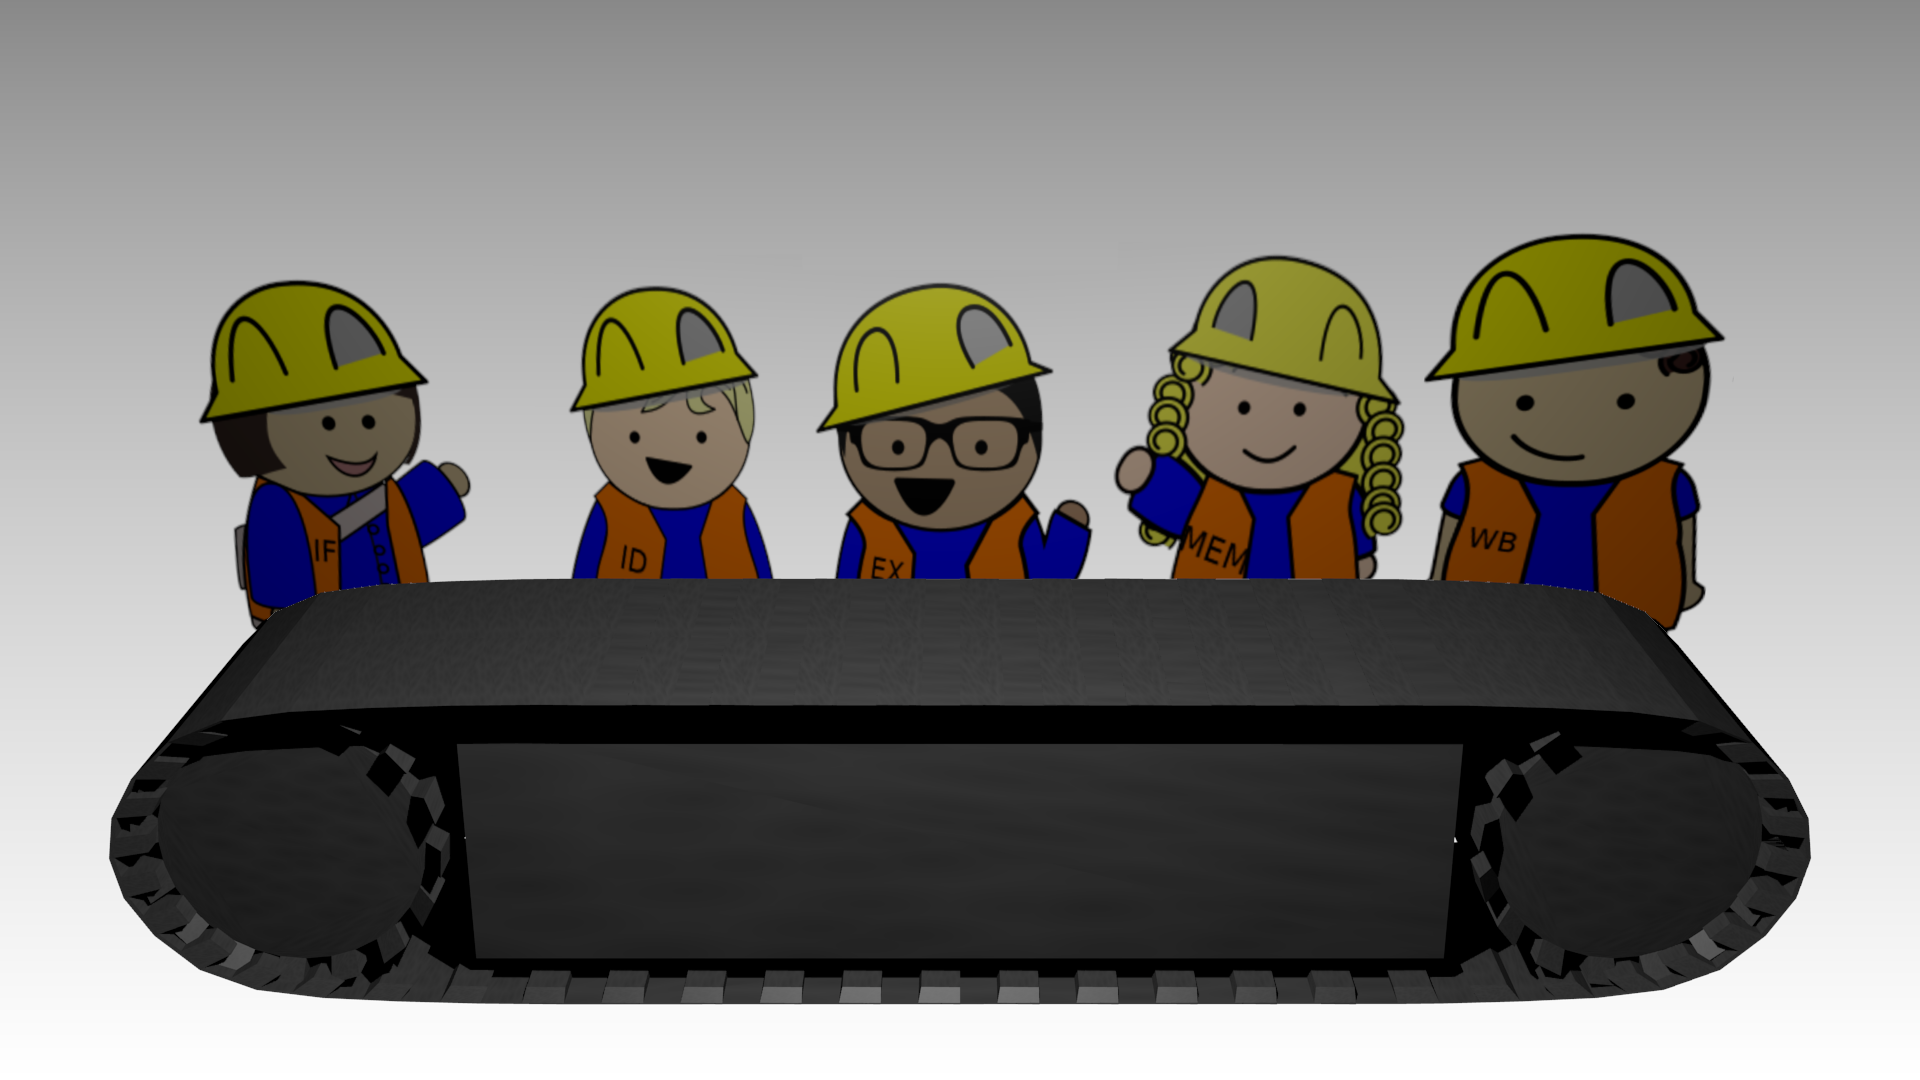
\includegraphics[width=1.0\textwidth]{final.png}}
	%FETCH
	\put(50,-12){\tiny\color{white}}
	
	%DECODE
	\put(90,-12){\tiny\color{white}}
	\put(90,-17){\tiny\color{white}}
	
	%EXECUTE
	\put(135,-12){\tiny\color{white}}
	\put(135,-17){\tiny\color{white}}
	\put(135,-22){\tiny\color{white}}
	
	%MEMORY
	\put(185,-12){\tiny\color{white}}
	\put(185,-17){\tiny\color{white}}
	\put(185,-22){\tiny\color{white}}
	
	%WRITEBACK
	\put(225,-12){\tiny\color{white}13:add t0, t0, 1}
	\put(225,-17){\tiny\color{white}13:t0 = 4 + 1}
	\put(225,-22){\tiny\color{white}13:t0 = 5}
	
	%REGISTERS
	\put(80,-37){\tiny\color{white}zero = 0}
	\put(80,-42){\tiny\color{white}ra = 0}
	\put(80,-47){\tiny\color{white}sp = 0}
	\put(80,-52){\tiny\color{white}pc = 68}
	\put(80,-57){\tiny\color{white}t0 = 5}
	\put(80,-62){\tiny\color{white}t1 = 0}
	
	\put(110,-37){\tiny\color{white}t2 = 0}
	\put(110,-42){\tiny\color{white}t3 = 0}
	\put(110,-47){\tiny\color{white}t4 = 0}
	\put(110,-52){\tiny\color{white}t5 = 0}
	\put(110,-57){\tiny\color{white}t6 = 0}
	\put(110,-62){\tiny\color{white}a0 = 0}
	
	\put(140,-37){\tiny\color{white}a1 = 0}
	\put(140,-42){\tiny\color{white}a2 = 0}
	\put(140,-47){\tiny\color{white}a3 = 0}
	\put(140,-52){\tiny\color{white}a4 = 0}
	\put(140,-57){\tiny\color{white}a5 = 0}
	\put(140,-62){\tiny\color{white}a6 = 0}
	
	\put(170,-37){\tiny\color{white}a7 = 0}
	\put(170,-42){\tiny\color{white}s1 = 0}
	\put(170,-47){\tiny\color{white}s2 = 0}
	\put(170,-52){\tiny\color{white}s3 = 0}
	\put(170,-57){\tiny\color{white}s4 = 0}
	\put(170,-62){\tiny\color{white}s5 = 0}
	
	\put(200,-37){\tiny\color{white}s6 = 0}
	\put(200,-42){\tiny\color{white}s7 = 0}
	\put(200,-47){\tiny\color{white}s8 = 0}
	\put(200,-52){\tiny\color{white}s9 = 0}
	\put(200,-57){\tiny\color{white}s10 = 0}
	\put(200,-62){\tiny\color{white}s11 = 0}
	
	\end{picture}
\end{frame}


\begin{frame}
	\frametitle{Pipeline Konfliktlösung: Takt 18}
	\begin{picture}(0,0)
	\put(0,-85){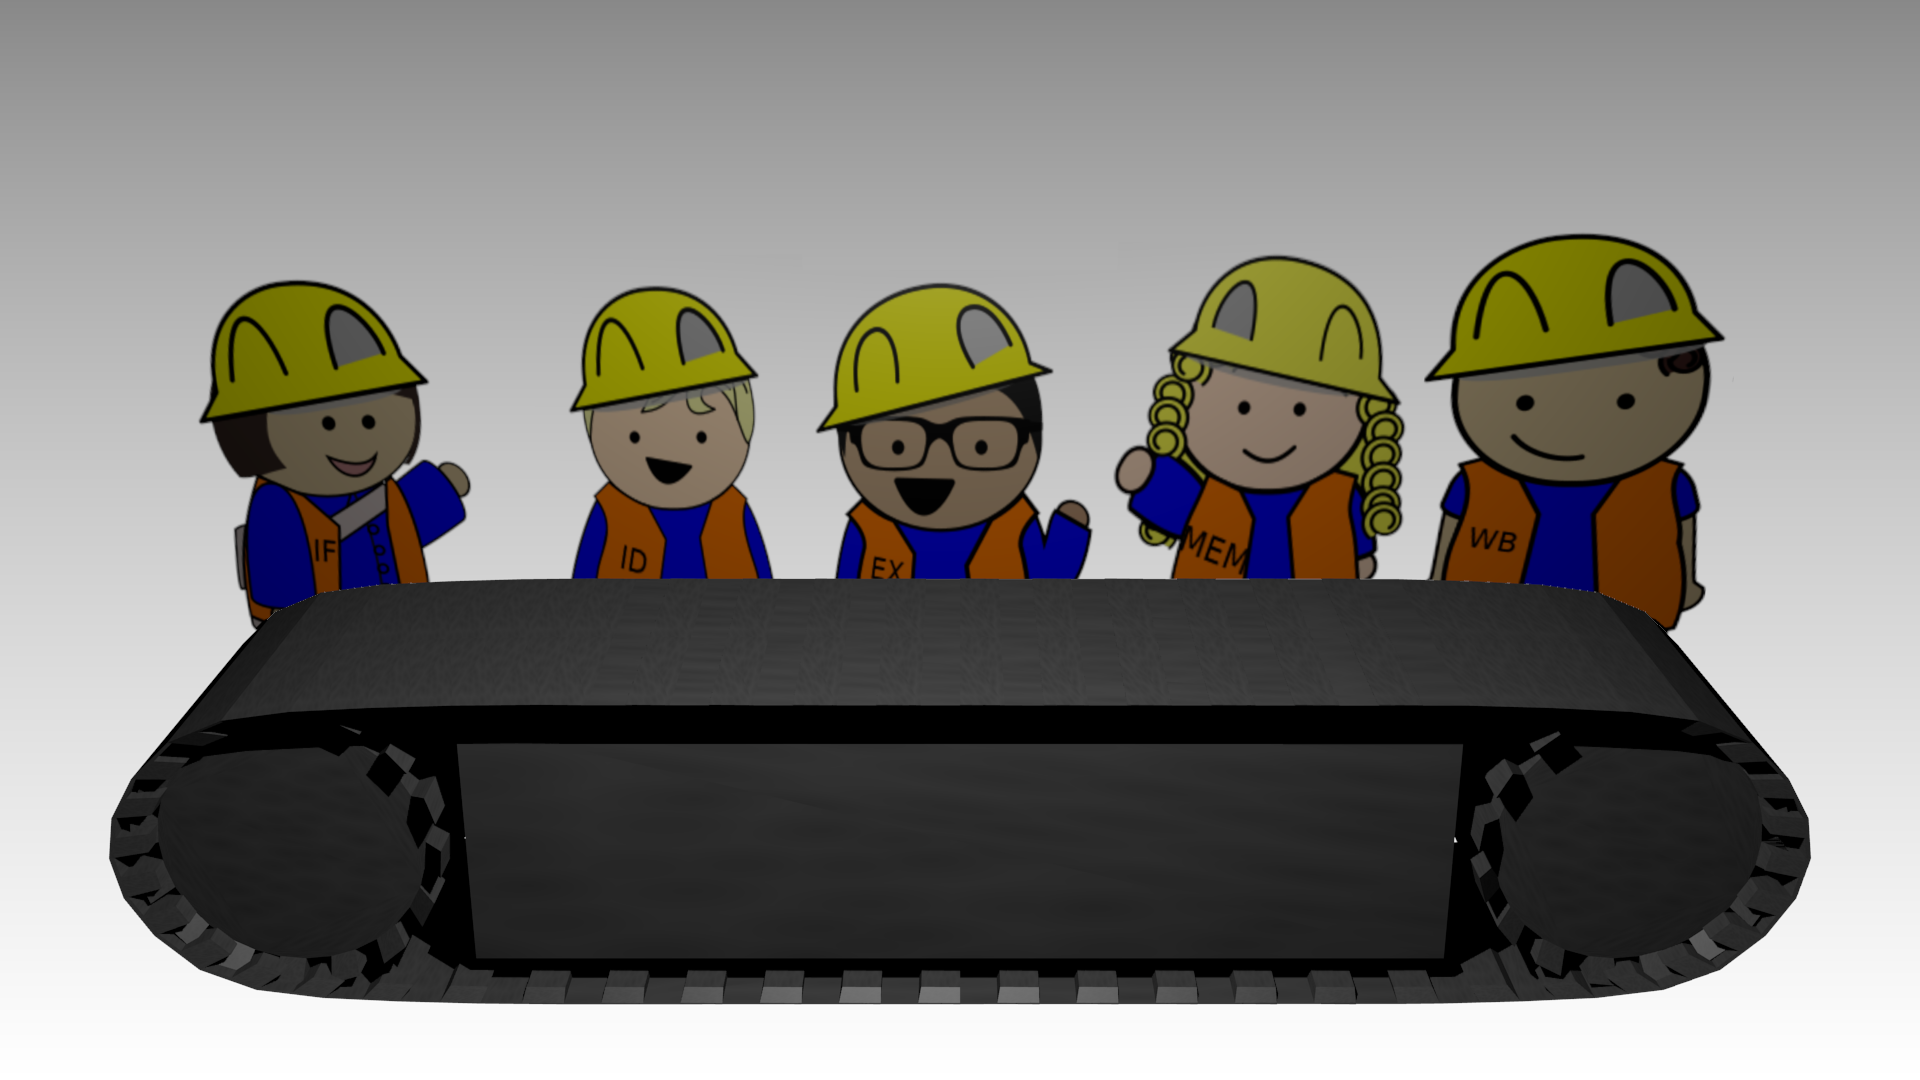
\includegraphics[width=1.0\textwidth]{final.png}}
	%FETCH
	\put(50,-12){\tiny\color{white}}
	
	%DECODE
	\put(90,-12){\tiny\color{white}}
	\put(90,-17){\tiny\color{white}}
	
	%EXECUTE
	\put(135,-12){\tiny\color{white}}
	\put(135,-17){\tiny\color{white}}
	\put(135,-22){\tiny\color{white}}
	
	%MEMORY
	\put(185,-12){\tiny\color{white}}
	\put(185,-17){\tiny\color{white}}
	\put(185,-22){\tiny\color{white}}
	
	%WRITEBACK
	\put(225,-12){\tiny\color{white}}
	\put(225,-17){\tiny\color{white}}
	\put(225,-22){\tiny\color{white}}
	
	%REGISTERS
	\put(80,-37){\tiny\color{white}zero = 0}
	\put(80,-42){\tiny\color{white}ra = 0}
	\put(80,-47){\tiny\color{white}sp = 0}
	\put(80,-52){\tiny\color{white}pc = 72}
	\put(80,-57){\tiny\color{white}t0 = 5}
	\put(80,-62){\tiny\color{white}t1 = 0}
	
	\put(110,-37){\tiny\color{white}t2 = 0}
	\put(110,-42){\tiny\color{white}t3 = 0}
	\put(110,-47){\tiny\color{white}t4 = 0}
	\put(110,-52){\tiny\color{white}t5 = 0}
	\put(110,-57){\tiny\color{white}t6 = 0}
	\put(110,-62){\tiny\color{white}a0 = 0}
	
	\put(140,-37){\tiny\color{white}a1 = 0}
	\put(140,-42){\tiny\color{white}a2 = 0}
	\put(140,-47){\tiny\color{white}a3 = 0}
	\put(140,-52){\tiny\color{white}a4 = 0}
	\put(140,-57){\tiny\color{white}a5 = 0}
	\put(140,-62){\tiny\color{white}a6 = 0}
	
	\put(170,-37){\tiny\color{white}a7 = 0}
	\put(170,-42){\tiny\color{white}s1 = 0}
	\put(170,-47){\tiny\color{white}s2 = 0}
	\put(170,-52){\tiny\color{white}s3 = 0}
	\put(170,-57){\tiny\color{white}s4 = 0}
	\put(170,-62){\tiny\color{white}s5 = 0}
	
	\put(200,-37){\tiny\color{white}s6 = 0}
	\put(200,-42){\tiny\color{white}s7 = 0}
	\put(200,-47){\tiny\color{white}s8 = 0}
	\put(200,-52){\tiny\color{white}s9 = 0}
	\put(200,-57){\tiny\color{white}s10 = 0}
	\put(200,-62){\tiny\color{white}s11 = 0}
	
	\end{picture}
\end{frame}


\end{document}

%%%%%%%%%%%%%%%%%%%%%%%%%%%%%%%%%%%%%%%%%%%%%%%%%%%%%%%%%%%%%%%%%%%%%%%%%%%%%%%
